% Options for packages loaded elsewhere
\PassOptionsToPackage{unicode}{hyperref}
\PassOptionsToPackage{hyphens}{url}
%
\documentclass[
]{article}
\usepackage{lmodern}
\usepackage{amssymb,amsmath}
\usepackage{ifxetex,ifluatex}
\ifnum 0\ifxetex 1\fi\ifluatex 1\fi=0 % if pdftex
  \usepackage[T1]{fontenc}
  \usepackage[utf8]{inputenc}
  \usepackage{textcomp} % provide euro and other symbols
\else % if luatex or xetex
  \usepackage{unicode-math}
  \defaultfontfeatures{Scale=MatchLowercase}
  \defaultfontfeatures[\rmfamily]{Ligatures=TeX,Scale=1}
\fi
% Use upquote if available, for straight quotes in verbatim environments
\IfFileExists{upquote.sty}{\usepackage{upquote}}{}
\IfFileExists{microtype.sty}{% use microtype if available
  \usepackage[]{microtype}
  \UseMicrotypeSet[protrusion]{basicmath} % disable protrusion for tt fonts
}{}
\makeatletter
\@ifundefined{KOMAClassName}{% if non-KOMA class
  \IfFileExists{parskip.sty}{%
    \usepackage{parskip}
  }{% else
    \setlength{\parindent}{0pt}
    \setlength{\parskip}{6pt plus 2pt minus 1pt}}
}{% if KOMA class
  \KOMAoptions{parskip=half}}
\makeatother
\usepackage{xcolor}
\IfFileExists{xurl.sty}{\usepackage{xurl}}{} % add URL line breaks if available
\IfFileExists{bookmark.sty}{\usepackage{bookmark}}{\usepackage{hyperref}}
\hypersetup{
  pdftitle={An Introduction to PGRdup Package},
  pdfauthor={Aravind, J.1, Radhamani, J.1, Kalyani Srinivasan1, Ananda Subhash, B.2, and Tyagi, R. K.1},
  hidelinks,
  pdfcreator={LaTeX via pandoc}}
\urlstyle{same} % disable monospaced font for URLs
\usepackage[margin=1in]{geometry}
\usepackage{color}
\usepackage{fancyvrb}
\newcommand{\VerbBar}{|}
\newcommand{\VERB}{\Verb[commandchars=\\\{\}]}
\DefineVerbatimEnvironment{Highlighting}{Verbatim}{commandchars=\\\{\}}
% Add ',fontsize=\small' for more characters per line
\usepackage{framed}
\definecolor{shadecolor}{RGB}{248,248,248}
\newenvironment{Shaded}{\begin{snugshade}}{\end{snugshade}}
\newcommand{\AlertTok}[1]{\textcolor[rgb]{0.94,0.16,0.16}{#1}}
\newcommand{\AnnotationTok}[1]{\textcolor[rgb]{0.56,0.35,0.01}{\textbf{\textit{#1}}}}
\newcommand{\AttributeTok}[1]{\textcolor[rgb]{0.77,0.63,0.00}{#1}}
\newcommand{\BaseNTok}[1]{\textcolor[rgb]{0.00,0.00,0.81}{#1}}
\newcommand{\BuiltInTok}[1]{#1}
\newcommand{\CharTok}[1]{\textcolor[rgb]{0.31,0.60,0.02}{#1}}
\newcommand{\CommentTok}[1]{\textcolor[rgb]{0.56,0.35,0.01}{\textit{#1}}}
\newcommand{\CommentVarTok}[1]{\textcolor[rgb]{0.56,0.35,0.01}{\textbf{\textit{#1}}}}
\newcommand{\ConstantTok}[1]{\textcolor[rgb]{0.00,0.00,0.00}{#1}}
\newcommand{\ControlFlowTok}[1]{\textcolor[rgb]{0.13,0.29,0.53}{\textbf{#1}}}
\newcommand{\DataTypeTok}[1]{\textcolor[rgb]{0.13,0.29,0.53}{#1}}
\newcommand{\DecValTok}[1]{\textcolor[rgb]{0.00,0.00,0.81}{#1}}
\newcommand{\DocumentationTok}[1]{\textcolor[rgb]{0.56,0.35,0.01}{\textbf{\textit{#1}}}}
\newcommand{\ErrorTok}[1]{\textcolor[rgb]{0.64,0.00,0.00}{\textbf{#1}}}
\newcommand{\ExtensionTok}[1]{#1}
\newcommand{\FloatTok}[1]{\textcolor[rgb]{0.00,0.00,0.81}{#1}}
\newcommand{\FunctionTok}[1]{\textcolor[rgb]{0.00,0.00,0.00}{#1}}
\newcommand{\ImportTok}[1]{#1}
\newcommand{\InformationTok}[1]{\textcolor[rgb]{0.56,0.35,0.01}{\textbf{\textit{#1}}}}
\newcommand{\KeywordTok}[1]{\textcolor[rgb]{0.13,0.29,0.53}{\textbf{#1}}}
\newcommand{\NormalTok}[1]{#1}
\newcommand{\OperatorTok}[1]{\textcolor[rgb]{0.81,0.36,0.00}{\textbf{#1}}}
\newcommand{\OtherTok}[1]{\textcolor[rgb]{0.56,0.35,0.01}{#1}}
\newcommand{\PreprocessorTok}[1]{\textcolor[rgb]{0.56,0.35,0.01}{\textit{#1}}}
\newcommand{\RegionMarkerTok}[1]{#1}
\newcommand{\SpecialCharTok}[1]{\textcolor[rgb]{0.00,0.00,0.00}{#1}}
\newcommand{\SpecialStringTok}[1]{\textcolor[rgb]{0.31,0.60,0.02}{#1}}
\newcommand{\StringTok}[1]{\textcolor[rgb]{0.31,0.60,0.02}{#1}}
\newcommand{\VariableTok}[1]{\textcolor[rgb]{0.00,0.00,0.00}{#1}}
\newcommand{\VerbatimStringTok}[1]{\textcolor[rgb]{0.31,0.60,0.02}{#1}}
\newcommand{\WarningTok}[1]{\textcolor[rgb]{0.56,0.35,0.01}{\textbf{\textit{#1}}}}
\usepackage{longtable,booktabs}
% Correct order of tables after \paragraph or \subparagraph
\usepackage{etoolbox}
\makeatletter
\patchcmd\longtable{\par}{\if@noskipsec\mbox{}\fi\par}{}{}
\makeatother
% Allow footnotes in longtable head/foot
\IfFileExists{footnotehyper.sty}{\usepackage{footnotehyper}}{\usepackage{footnote}}
\makesavenoteenv{longtable}
\usepackage{graphicx,grffile}
\makeatletter
\def\maxwidth{\ifdim\Gin@nat@width>\linewidth\linewidth\else\Gin@nat@width\fi}
\def\maxheight{\ifdim\Gin@nat@height>\textheight\textheight\else\Gin@nat@height\fi}
\makeatother
% Scale images if necessary, so that they will not overflow the page
% margins by default, and it is still possible to overwrite the defaults
% using explicit options in \includegraphics[width, height, ...]{}
\setkeys{Gin}{width=\maxwidth,height=\maxheight,keepaspectratio}
% Set default figure placement to htbp
\makeatletter
\def\fps@figure{htbp}
\makeatother
\setlength{\emergencystretch}{3em} % prevent overfull lines
\providecommand{\tightlist}{%
  \setlength{\itemsep}{0pt}\setlength{\parskip}{0pt}}
\setcounter{secnumdepth}{-\maxdimen} % remove section numbering
\usepackage{fancyhdr}
\usepackage{wrapfig}
\pagestyle{fancy}
\fancyhead[LE,RO]{\slshape \rightmark}
\fancyhead[LO,RE]{An Introduction to \texttt{PGRdup} Package}
\fancyfoot[C]{\thepage}
\usepackage{hyperref}
\hypersetup{colorlinks=true}
\hypersetup{linktoc=all}
\hypersetup{linkcolor=blue}

\title{An Introduction to \texttt{PGRdup} Package}
\author{Aravind, J.\textsuperscript{1}, Radhamani, J.\textsuperscript{1},
Kalyani Srinivasan\textsuperscript{1}, Ananda Subhash,
B.\textsuperscript{2}, and Tyagi, R. K.\textsuperscript{1}}
\date{2020-07-26}

\begin{document}
\maketitle

\begin{center}
1. ICAR-National Bureau of Plant Genetic Resources, New Delhi, India.

2. Centre for Development of Advanced Computing, Thiruvananthapuram, Kerala, India.

\end{center}

\begin{center}
\vspace{6pt}
\hrule
\end{center}

\tableofcontents

\begin{wrapfigure}{r}{0.35\textwidth}
  \vspace{1cm}
  \begin{center}
    
\includegraphics[width=0.33\textwidth]{D:/Program Files/R/R-devel/library/PGRdup/extdata/PGRdup_v2.png}
  \end{center}
  \vspace{-1.5cm}
\end{wrapfigure}\leavevmode

\hypertarget{introduction}{%
\subsection{Introduction}\label{introduction}}

\textbf{PGRdup} is an \texttt{R} package to facilitate the search for
probable/possible duplicate accessions in Plant Genetic Resources (PGR)
collections using passport databases. Primarily this package implements
a workflow (Fig.~1) designed to fetch groups or sets of germplasm
accessions with similar passport data particularly in fields associated
with accession names within or across PGR passport databases. It offers
a suite of functions for data pre-processing, creation of a searchable
Key Word in Context (KWIC) index of keywords associated with accession
records and the identification of probable duplicate sets by fuzzy,
phonetic and semantic matching of keywords. It also has functions to
enable the user to review, modify and validate the probable duplicate
sets retrieved.

The goal of this document is to introduce the users to these functions
and familiarise them with the workflow intended to fetch probable
duplicate sets. This document assumes a basic knowledge of \texttt{R}
programming language.

The functions in this package are primarily built using the \texttt{R}
packages
\href{https://CRAN.R-project.org/package=data.table}{\texttt{data.table}},
\href{https://CRAN.R-project.org/package=igraph}{\texttt{igraph}},
\href{https://CRAN.R-project.org/package=stringdist}{\texttt{stringdist}}
and \href{https://CRAN.R-project.org/package=stringi}{\texttt{stringi}}.

\clearpage
\pagebreak

\begin{center}
    
\includegraphics{D:/Program Files/R/R-devel/library/PGRdup/extdata/PGRdup.png}
\end{center}

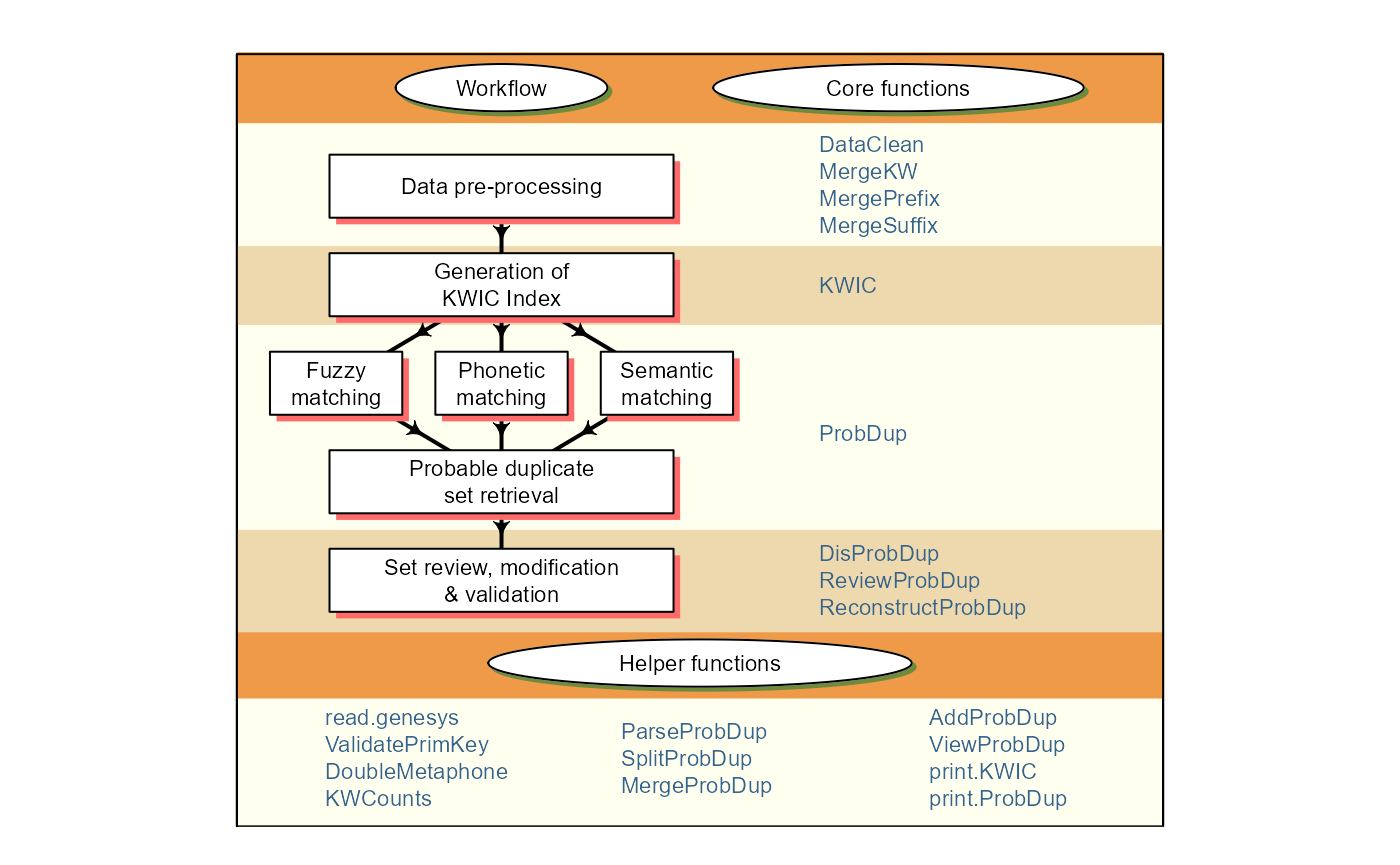
\includegraphics{Introduction_files/figure-latex/unnamed-chunk-5-1.pdf}

\textbf{Fig. 1.} PGRdup workflow and associated functions

\hypertarget{version-history}{%
\subsection{Version History}\label{version-history}}

The current version of the package is 0.2.3.6. The previous versions are
as follows.

\textbf{Table 1.} Version history of \texttt{PGRdup} \texttt{R} package.

\begin{longtable}[]{@{}ll@{}}
\toprule
Version & Date\tabularnewline
\midrule
\endhead
0.2 & 2015-04-14\tabularnewline
0.2.1 & 2015-07-23\tabularnewline
0.2.2 & 2016-03-05\tabularnewline
0.2.2.1 & 2016-03-09\tabularnewline
0.2.3 & 2017-02-01\tabularnewline
0.2.3.1 & 2017-03-15\tabularnewline
0.2.3.2 & 2017-08-05\tabularnewline
0.2.3.3 & 2018-01-13\tabularnewline
0.2.3.4 & 2019-09-19\tabularnewline
0.2.3.5 & 2020-02-10\tabularnewline
\bottomrule
\end{longtable}

To know detailed history of changes use
\texttt{news(package=\textquotesingle{}PGRdup\textquotesingle{})}.

\pagebreak

\hypertarget{installation}{%
\subsection{Installation}\label{installation}}

The package can be installed using the following functions:

\begin{Shaded}
\begin{Highlighting}[]
\CommentTok{# Install from CRAN}
\KeywordTok{install.packages}\NormalTok{(}\StringTok{'PGRdup'}\NormalTok{, }\DataTypeTok{dependencies=}\OtherTok{TRUE}\NormalTok{)}
\end{Highlighting}
\end{Shaded}

Uninstalled dependencies (packages which \texttt{PGRdup} depends on
\emph{viz}-
\href{https://CRAN.R-project.org/package=data.table}{\texttt{data.table}},
\href{https://CRAN.R-project.org/package=igraph}{\texttt{igraph}},
\href{https://CRAN.R-project.org/package=stringdist}{\texttt{stringdist}}
and \href{https://CRAN.R-project.org/package=stringi}{\texttt{stringi}}
are also installed because of the argument \texttt{dependencies=TRUE}.

Then the package can be loaded using the function

\begin{Shaded}
\begin{Highlighting}[]
\KeywordTok{library}\NormalTok{(PGRdup)}
\end{Highlighting}
\end{Shaded}

\hypertarget{data-format}{%
\subsection{Data Format}\label{data-format}}

The package is essentially designed to operate on PGR passport data
present in a \href{http://google.com/\#q=\%5BR\%5D+data.frame}{data
frame object}, with each row holding one record and columns representing
the attribute fields. For example, consider the dataset \texttt{GN1000}
supplied along with the package.

\begin{Shaded}
\begin{Highlighting}[]
\KeywordTok{library}\NormalTok{(PGRdup)}
\CommentTok{# Load the dataset to the environment}
\KeywordTok{data}\NormalTok{(GN1000)}
\CommentTok{# Show the class of the object}
\KeywordTok{class}\NormalTok{(GN1000)}
\end{Highlighting}
\end{Shaded}

\begin{verbatim}
[1] "data.frame"
\end{verbatim}

\begin{Shaded}
\begin{Highlighting}[]
\CommentTok{# View the first few records in the data frame}
\KeywordTok{head}\NormalTok{(GN1000)}
\end{Highlighting}
\end{Shaded}

\begin{verbatim}
  CommonName    BotanicalName NationalID                CollNo   DonorID OtherID1  OtherID2 BioStatus
1  Groundnut Arachis hypogaea   EC100277 Shulamith/ NRCG-14555  ICG-4709           U4-47-12  Landrace
2  Groundnut Arachis hypogaea   EC100280                    NC   ICG5288      NCS      NC 5  Landrace
3  Groundnut Arachis hypogaea   EC100281               MALIMBA   ICG5289          EC 100281  Landrace
4  Groundnut Arachis hypogaea   EC100713            EC 100713;   ICG5296              STARR  Landrace
5  Groundnut Arachis hypogaea   EC100715             EC 100715   ICG5298              COMET  Landrace
6  Groundnut Arachis hypogaea   EC100716                        ICG-3150          ARGENTINE  Landrace
             SourceCountry TransferYear
1                   Israel         2014
2 United States of America         2004
3                   Malawi         2004
4 United States of America         2004
5 United States of America         2004
6 United States of America         2014
\end{verbatim}

If the passport data exists as an excel sheet, it can be first converted
to a comma-separated values (csv) file or tab delimited file and then
easily imported into the \texttt{R} environment using the base functions
\texttt{read.csv} and \texttt{read.table} respectively. Similarly
\texttt{read\_csv()} and \texttt{read\_tsv()} from the
\href{https://CRAN.R-project.org/package=readr}{\texttt{readr}} package
can also be used. Alternatively, the package
\href{https://CRAN.R-project.org/package=readxl}{\texttt{readxl}} can be
used to directly read the data from excel. In case of large csv files,
the function \texttt{fread} in the
\href{https://CRAN.R-project.org/package=data.table}{\texttt{data.table}}
package can be used to rapidly load the data.

If the PGR passport data is in a database management system (DBMS), the
required table can be imported as a data frame into \texttt{R}. using
the appropriate
\href{http://www.burns-stat.com/r-database-interfaces/}{\texttt{R}-database
interface package}. For example
\href{https://CRAN.R-project.org/package=dbConnect}{\texttt{dbConnect}}
for MySQL,
\href{https://CRAN.R-project.org/package=ROracle}{\texttt{ROracle}} for
Oracle etc.

The PGR data downloaded from the
\href{https://www.genesys-pgr.org/welcome}{genesys} database as a
\href{https://github.com/dagendresen/darwincore-germplasm}{Darwin Core -
Germplasm} zip archive can be imported into the \texttt{R} environment
as a flat file \texttt{data.frame} using the \texttt{read.genesys}
function.

\begin{Shaded}
\begin{Highlighting}[]
\CommentTok{# Import the DwC-Germplasm zip archive "genesys-accessions-filtered.zip"}
\NormalTok{PGRgenesys <-}\StringTok{ }\KeywordTok{read.genesys}\NormalTok{(}\StringTok{"genesys-accessions-filtered.zip"}\NormalTok{,}
                           \DataTypeTok{scrub.names.space =} \OtherTok{TRUE}\NormalTok{, }\DataTypeTok{readme =} \OtherTok{TRUE}\NormalTok{)}
\end{Highlighting}
\end{Shaded}

\hypertarget{data-pre-processing}{%
\subsection{Data Pre-processing}\label{data-pre-processing}}

Data pre-processing is a critical step which can affect the quality of
the probable duplicate sets being retrieved. It involves data
standardization as well as data cleaning which can be achieved using the
functions \texttt{DataClean}, \texttt{MergeKW}, \texttt{MergePrefix} and
\texttt{MergeSuffix}.

\texttt{DataClean} function can be used to clean the character strings
in passport data fields(columns) specified as the input
\href{http://google.com/\#q=\%5BR\%5D+character+vector}{character
vector} \texttt{x} according to the conditions specified in the
arguments.

Commas, semicolons and colons which are sometimes used to separate
multiple strings or names within the same field can be replaced with a
single space using the logical arguments \texttt{fix.comma},
\texttt{fix.semcol} and \texttt{fix.col} respectively.

\begin{Shaded}
\begin{Highlighting}[]
\NormalTok{x <-}\StringTok{ }\KeywordTok{c}\NormalTok{(}\StringTok{"A 14; EC 1697"}\NormalTok{, }\StringTok{"U 4-4-28; EC 21078; A 32"}\NormalTok{, }\StringTok{"PI 262801:CIAT 9075:GKP 9553/90"}\NormalTok{,}
       \StringTok{"NCAC 16049, PI 261987, RCM 493-3"}\NormalTok{)}
\NormalTok{x}
\end{Highlighting}
\end{Shaded}

\begin{verbatim}
[1] "A 14; EC 1697"                    "U 4-4-28; EC 21078; A 32"         "PI 262801:CIAT 9075:GKP 9553/90" 
[4] "NCAC 16049, PI 261987, RCM 493-3"
\end{verbatim}

\begin{Shaded}
\begin{Highlighting}[]
\CommentTok{# Replace ',', ':' and ';' with space}
\KeywordTok{DataClean}\NormalTok{(x, }\DataTypeTok{fix.comma=}\OtherTok{TRUE}\NormalTok{, }\DataTypeTok{fix.semcol=}\OtherTok{TRUE}\NormalTok{, }\DataTypeTok{fix.col=}\OtherTok{TRUE}\NormalTok{,}
          \DataTypeTok{fix.bracket=}\OtherTok{FALSE}\NormalTok{, }\DataTypeTok{fix.punct=}\OtherTok{FALSE}\NormalTok{, }\DataTypeTok{fix.space=}\OtherTok{FALSE}\NormalTok{, }\DataTypeTok{fix.sep=}\OtherTok{FALSE}\NormalTok{,}
          \DataTypeTok{fix.leadzero=}\OtherTok{FALSE}\NormalTok{)}
\end{Highlighting}
\end{Shaded}

\begin{verbatim}
[1] "A 14  EC 1697"                    "U 4-4-28  EC 21078  A 32"         "PI 262801 CIAT 9075 GKP 9553/90" 
[4] "NCAC 16049  PI 261987  RCM 493-3"
\end{verbatim}

Similarly the logical argument \texttt{fix.bracket} can be used to
replace all brackets including parenthesis, square brackets and curly
brackets with space.

\begin{Shaded}
\begin{Highlighting}[]
\NormalTok{x <-}\StringTok{ }\KeywordTok{c}\NormalTok{(}\StringTok{"(NRCG-1738)/(NFG649)"}\NormalTok{, }\StringTok{"26-5-1[NRCG-2528]"}\NormalTok{, }\StringTok{"Ah 1182 \{NRCG-4340\}"}\NormalTok{)}
\NormalTok{x}
\end{Highlighting}
\end{Shaded}

\begin{verbatim}
[1] "(NRCG-1738)/(NFG649)" "26-5-1[NRCG-2528]"    "Ah 1182 {NRCG-4340}" 
\end{verbatim}

\begin{Shaded}
\begin{Highlighting}[]
\CommentTok{# Replace parenthesis, square brackets and curly brackets with space}
\KeywordTok{DataClean}\NormalTok{(x, }\DataTypeTok{fix.comma=}\OtherTok{FALSE}\NormalTok{, }\DataTypeTok{fix.semcol=}\OtherTok{FALSE}\NormalTok{, }\DataTypeTok{fix.col=}\OtherTok{FALSE}\NormalTok{,}
          \DataTypeTok{fix.bracket=}\OtherTok{TRUE}\NormalTok{,}
          \DataTypeTok{fix.punct=}\OtherTok{FALSE}\NormalTok{, }\DataTypeTok{fix.space=}\OtherTok{FALSE}\NormalTok{, }\DataTypeTok{fix.sep=}\OtherTok{FALSE}\NormalTok{, }\DataTypeTok{fix.leadzero=}\OtherTok{FALSE}\NormalTok{)}
\end{Highlighting}
\end{Shaded}

\begin{verbatim}
[1] "NRCG-1738 / NFG649" "26-5-1 NRCG-2528"   "AH 1182  NRCG-4340"
\end{verbatim}

The logical argument \texttt{fix.punct} can be used to remove all
punctuation from the data.

\begin{Shaded}
\begin{Highlighting}[]
\NormalTok{x <-}\StringTok{ }\KeywordTok{c}\NormalTok{(}\StringTok{"#26-6-3-1"}\NormalTok{, }\StringTok{"Culture No. 857"}\NormalTok{, }\StringTok{"U/4/47/13"}\NormalTok{)}
\NormalTok{x}
\end{Highlighting}
\end{Shaded}

\begin{verbatim}
[1] "#26-6-3-1"       "Culture No. 857" "U/4/47/13"      
\end{verbatim}

\begin{Shaded}
\begin{Highlighting}[]
\CommentTok{# Remove punctuation}
\KeywordTok{DataClean}\NormalTok{(x, }\DataTypeTok{fix.comma=}\OtherTok{FALSE}\NormalTok{, }\DataTypeTok{fix.semcol=}\OtherTok{FALSE}\NormalTok{, }\DataTypeTok{fix.col=}\OtherTok{FALSE}\NormalTok{, }\DataTypeTok{fix.bracket=}\OtherTok{FALSE}\NormalTok{,}
          \DataTypeTok{fix.punct=}\OtherTok{TRUE}\NormalTok{,}
          \DataTypeTok{fix.space=}\OtherTok{FALSE}\NormalTok{, }\DataTypeTok{fix.sep=}\OtherTok{FALSE}\NormalTok{, }\DataTypeTok{fix.leadzero=}\OtherTok{FALSE}\NormalTok{)}
\end{Highlighting}
\end{Shaded}

\begin{verbatim}
[1] "26631"          "CULTURE NO 857" "U44713"        
\end{verbatim}

\texttt{fix.space} can be used to convert all space characters such as
tab, newline, vertical tab, form feed and carriage return to spaces and
finally convert multiple spaces to single space.

\begin{Shaded}
\begin{Highlighting}[]
\NormalTok{x <-}\StringTok{ }\KeywordTok{c}\NormalTok{(}\StringTok{"RS   1"}\NormalTok{, }\StringTok{"GKSPScGb 208  PI 475855"}\NormalTok{)}
\NormalTok{x}
\end{Highlighting}
\end{Shaded}

\begin{verbatim}
[1] "RS   1"                  "GKSPScGb 208  PI 475855"
\end{verbatim}

\begin{Shaded}
\begin{Highlighting}[]
\CommentTok{# Replace all space characters to space and convert multiple spaces to single space}
\KeywordTok{DataClean}\NormalTok{(x, }\DataTypeTok{fix.comma=}\OtherTok{FALSE}\NormalTok{, }\DataTypeTok{fix.semcol=}\OtherTok{FALSE}\NormalTok{, }\DataTypeTok{fix.col=}\OtherTok{FALSE}\NormalTok{,}
          \DataTypeTok{fix.bracket=}\OtherTok{FALSE}\NormalTok{, }\DataTypeTok{fix.punct=}\OtherTok{FALSE}\NormalTok{,}
          \DataTypeTok{fix.space=}\OtherTok{TRUE}\NormalTok{,}
          \DataTypeTok{fix.sep=}\OtherTok{FALSE}\NormalTok{, }\DataTypeTok{fix.leadzero=}\OtherTok{FALSE}\NormalTok{)}
\end{Highlighting}
\end{Shaded}

\begin{verbatim}
[1] "RS 1"                   "GKSPSCGB 208 PI 475855"
\end{verbatim}

\texttt{fix.sep} can be used to merge together accession identifiers
composed of alphabetic characters separated from a series of digits by a
space character.

\begin{Shaded}
\begin{Highlighting}[]
\NormalTok{x <-}\StringTok{ }\KeywordTok{c}\NormalTok{(}\StringTok{"NCAC 18078"}\NormalTok{, }\StringTok{"AH 6481"}\NormalTok{, }\StringTok{"ICG 2791"}\NormalTok{)}
\NormalTok{x}
\end{Highlighting}
\end{Shaded}

\begin{verbatim}
[1] "NCAC 18078" "AH 6481"    "ICG 2791"  
\end{verbatim}

\begin{Shaded}
\begin{Highlighting}[]
\CommentTok{# Merge alphabetic character separated from a series of digits by a space}
\KeywordTok{DataClean}\NormalTok{(x, }\DataTypeTok{fix.comma=}\OtherTok{FALSE}\NormalTok{, }\DataTypeTok{fix.semcol=}\OtherTok{FALSE}\NormalTok{, }\DataTypeTok{fix.col=}\OtherTok{FALSE}\NormalTok{,}
          \DataTypeTok{fix.bracket=}\OtherTok{FALSE}\NormalTok{, }\DataTypeTok{fix.punct=}\OtherTok{FALSE}\NormalTok{, }\DataTypeTok{fix.space=}\OtherTok{FALSE}\NormalTok{,}
          \DataTypeTok{fix.sep=}\OtherTok{TRUE}\NormalTok{,}
          \DataTypeTok{fix.leadzero=}\OtherTok{FALSE}\NormalTok{)}
\end{Highlighting}
\end{Shaded}

\begin{verbatim}
[1] "NCAC18078" "AH6481"    "ICG2791"  
\end{verbatim}

\texttt{fix.leadzero} can be used to remove leading zeros from accession
name fields to facilitate matching to identify probable duplicates.

\begin{Shaded}
\begin{Highlighting}[]
\NormalTok{x <-}\StringTok{ }\KeywordTok{c}\NormalTok{(}\StringTok{"EC 0016664"}\NormalTok{, }\StringTok{"EC0001690"}\NormalTok{)}
\NormalTok{x}
\end{Highlighting}
\end{Shaded}

\begin{verbatim}
[1] "EC 0016664" "EC0001690" 
\end{verbatim}

\begin{Shaded}
\begin{Highlighting}[]
\CommentTok{# Remove leading zeros}
\KeywordTok{DataClean}\NormalTok{(x, }\DataTypeTok{fix.comma=}\OtherTok{FALSE}\NormalTok{, }\DataTypeTok{fix.semcol=}\OtherTok{FALSE}\NormalTok{, }\DataTypeTok{fix.col=}\OtherTok{FALSE}\NormalTok{,}
          \DataTypeTok{fix.bracket=}\OtherTok{FALSE}\NormalTok{, }\DataTypeTok{fix.punct=}\OtherTok{FALSE}\NormalTok{, }\DataTypeTok{fix.space=}\OtherTok{FALSE}\NormalTok{, }\DataTypeTok{fix.sep=}\OtherTok{FALSE}\NormalTok{,}
          \DataTypeTok{fix.leadzero=}\OtherTok{TRUE}\NormalTok{)}
\end{Highlighting}
\end{Shaded}

\begin{verbatim}
[1] "EC 16664" "EC1690"  
\end{verbatim}

This function can hence be made use of in tidying up multiple forms of
messy data existing in fields associated with accession names in PGR
passport databases (Table~1).

\begin{Shaded}
\begin{Highlighting}[]
\NormalTok{names <-}\StringTok{ }\KeywordTok{c}\NormalTok{(}\StringTok{"S7-12-6"}\NormalTok{, }\StringTok{"ICG-3505"}\NormalTok{, }\StringTok{"U 4-47-18;EC 21127"}\NormalTok{, }\StringTok{"AH 6481"}\NormalTok{, }\StringTok{"RS   1"}\NormalTok{,}
           \StringTok{"AK 12-24"}\NormalTok{, }\StringTok{"2-5 (NRCG-4053)"}\NormalTok{, }\StringTok{"T78, Mwitunde"}\NormalTok{, }\StringTok{"ICG 3410"}\NormalTok{,}
           \StringTok{"#648-4 (Gwalior)"}\NormalTok{, }\StringTok{"TG4;U/4/47/13"}\NormalTok{, }\StringTok{"EC0021003"}\NormalTok{)}
\NormalTok{names}
\end{Highlighting}
\end{Shaded}

\begin{verbatim}
 [1] "S7-12-6"            "ICG-3505"           "U 4-47-18;EC 21127" "AH 6481"            "RS   1"            
 [6] "AK 12-24"           "2-5 (NRCG-4053)"    "T78, Mwitunde"      "ICG 3410"           "#648-4 (Gwalior)"  
[11] "TG4;U/4/47/13"      "EC0021003"         
\end{verbatim}

\begin{Shaded}
\begin{Highlighting}[]
\CommentTok{# Clean the data}
\KeywordTok{DataClean}\NormalTok{(names)}
\end{Highlighting}
\end{Shaded}

\begin{verbatim}
 [1] "S7126"          "ICG3505"        "U44718 EC21127" "AH6481"         "RS1"            "AK1224"        
 [7] "25 NRCG4053"    "T78 MWITUNDE"   "ICG3410"        "6484 GWALIOR"   "TG4 U44713"     "EC21003"       
\end{verbatim}

\textbf{Table 2.} Data pre-processing using \texttt{DataClean}.

\begin{longtable}[]{@{}ll@{}}
\toprule
\textbf{names} & \textbf{DataClean(names)}\tabularnewline
\midrule
\endhead
S7-12-6 & S7126\tabularnewline
ICG-3505 & ICG3505\tabularnewline
U 4-47-18;EC 21127 & U44718 EC21127\tabularnewline
AH 6481 & AH6481\tabularnewline
RS 1 & RS1\tabularnewline
AK 12-24 & AK1224\tabularnewline
2-5 (NRCG-4053) & 25 NRCG4053\tabularnewline
T78, Mwitunde & T78 MWITUNDE\tabularnewline
ICG 3410 & ICG3410\tabularnewline
\#648-4 (Gwalior) & 6484 GWALIOR\tabularnewline
TG4;U/4/47/13 & TG4 U44713\tabularnewline
EC0021003 & EC21003\tabularnewline
\bottomrule
\end{longtable}

Several common keyword string pairs or keyword prefixes and suffixes
exist in fields associated with accession names in PGR passport
databases. They can be merged using the functions \texttt{MergeKW},
\texttt{MergePrefix} and \texttt{MergeSuffix} respectively. The keyword
string pairs, prefixes and suffixes can be supplied as a
\href{http://google.com/\#q=\%5BR\%5D+list}{list} or a
\href{http://google.com/\#q=\%5BR\%5D+vector}{vector} to the argument
\texttt{y} in these functions.

\begin{Shaded}
\begin{Highlighting}[]
\NormalTok{names <-}\StringTok{ }\KeywordTok{c}\NormalTok{(}\StringTok{"Punjab Bold"}\NormalTok{, }\StringTok{"Gujarat- Dwarf"}\NormalTok{, }\StringTok{"Nagpur.local"}\NormalTok{, }\StringTok{"SAM COL 144"}\NormalTok{,}
           \StringTok{"SAM COL--280"}\NormalTok{, }\StringTok{"NIZAMABAD-LOCAL"}\NormalTok{, }\StringTok{"Dark Green Mutant"}\NormalTok{,}
           \StringTok{"Dixie-Giant"}\NormalTok{, }\StringTok{"Georgia- Bunch"}\NormalTok{, }\StringTok{"Uganda-erect"}\NormalTok{, }\StringTok{"Small Japan"}\NormalTok{,}
           \StringTok{"Castle  Cary"}\NormalTok{, }\StringTok{"Punjab erect"}\NormalTok{, }\StringTok{"Improved small japan"}\NormalTok{,}
           \StringTok{"Dark Purple"}\NormalTok{)}
\NormalTok{names}
\end{Highlighting}
\end{Shaded}

\begin{verbatim}
 [1] "Punjab Bold"          "Gujarat- Dwarf"       "Nagpur.local"         "SAM COL 144"          "SAM COL--280"        
 [6] "NIZAMABAD-LOCAL"      "Dark Green Mutant"    "Dixie-Giant"          "Georgia- Bunch"       "Uganda-erect"        
[11] "Small Japan"          "Castle  Cary"         "Punjab erect"         "Improved small japan" "Dark Purple"         
\end{verbatim}

\begin{Shaded}
\begin{Highlighting}[]
\CommentTok{# Merge pairs of strings}
\NormalTok{y1 <-}\StringTok{ }\KeywordTok{list}\NormalTok{(}\KeywordTok{c}\NormalTok{(}\StringTok{"Gujarat"}\NormalTok{, }\StringTok{"Dwarf"}\NormalTok{), }\KeywordTok{c}\NormalTok{(}\StringTok{"Castle"}\NormalTok{, }\StringTok{"Cary"}\NormalTok{), }\KeywordTok{c}\NormalTok{(}\StringTok{"Small"}\NormalTok{, }\StringTok{"Japan"}\NormalTok{),}
           \KeywordTok{c}\NormalTok{(}\StringTok{"Big"}\NormalTok{, }\StringTok{"Japan"}\NormalTok{), }\KeywordTok{c}\NormalTok{(}\StringTok{"Mani"}\NormalTok{, }\StringTok{"Blanco"}\NormalTok{), }\KeywordTok{c}\NormalTok{(}\StringTok{"Uganda"}\NormalTok{, }\StringTok{"Erect"}\NormalTok{),}
           \KeywordTok{c}\NormalTok{(}\StringTok{"Mota"}\NormalTok{, }\StringTok{"Company"}\NormalTok{))}
\NormalTok{names <-}\StringTok{ }\KeywordTok{MergeKW}\NormalTok{(names, y1, }\DataTypeTok{delim =} \KeywordTok{c}\NormalTok{(}\StringTok{"space"}\NormalTok{, }\StringTok{"dash"}\NormalTok{, }\StringTok{"period"}\NormalTok{))}

\CommentTok{# Merge prefix strings}
\NormalTok{y2 <-}\StringTok{ }\KeywordTok{c}\NormalTok{(}\StringTok{"Light"}\NormalTok{, }\StringTok{"Small"}\NormalTok{, }\StringTok{"Improved"}\NormalTok{, }\StringTok{"Punjab"}\NormalTok{, }\StringTok{"SAM"}\NormalTok{, }\StringTok{"Dark"}\NormalTok{)}
\NormalTok{names <-}\StringTok{ }\KeywordTok{MergePrefix}\NormalTok{(names, y2, }\DataTypeTok{delim =} \KeywordTok{c}\NormalTok{(}\StringTok{"space"}\NormalTok{, }\StringTok{"dash"}\NormalTok{, }\StringTok{"period"}\NormalTok{))}

\CommentTok{# Merge suffix strings}
\NormalTok{y3 <-}\StringTok{ }\KeywordTok{c}\NormalTok{(}\StringTok{"Local"}\NormalTok{, }\StringTok{"Bold"}\NormalTok{, }\StringTok{"Cary"}\NormalTok{, }\StringTok{"Mutant"}\NormalTok{, }\StringTok{"Runner"}\NormalTok{, }\StringTok{"Giant"}\NormalTok{, }\StringTok{"No."}\NormalTok{,}
        \StringTok{"Bunch"}\NormalTok{, }\StringTok{"Peanut"}\NormalTok{)}
\NormalTok{names <-}\StringTok{ }\KeywordTok{MergeSuffix}\NormalTok{(names, y3, }\DataTypeTok{delim =} \KeywordTok{c}\NormalTok{(}\StringTok{"space"}\NormalTok{, }\StringTok{"dash"}\NormalTok{, }\StringTok{"period"}\NormalTok{))}

\NormalTok{names}
\end{Highlighting}
\end{Shaded}

\begin{verbatim}
 [1] "PunjabBold"         "GujaratDwarf"       "Nagpurlocal"        "SAMCOL 144"         "SAMCOL--280"       
 [6] "NIZAMABADLOCAL"     "DarkGreenMutant"    "DixieGiant"         "GeorgiaBunch"       "Ugandaerect"       
[11] "SmallJapan"         "CastleCary"         "Punjaberect"        "Improvedsmalljapan" "DarkPurple"        
\end{verbatim}

These functions can be applied over multiple columns(fields) in a data
frame using the
\href{http://google.com/\#q=\%5BR\%5D+lapply}{\texttt{lapply}} function.

\begin{Shaded}
\begin{Highlighting}[]
\CommentTok{# Load example dataset}
\NormalTok{GN <-}\StringTok{ }\NormalTok{GN1000}

\CommentTok{# Specify as a vector the database fields to be used}
\NormalTok{GNfields <-}\StringTok{ }\KeywordTok{c}\NormalTok{(}\StringTok{"NationalID"}\NormalTok{, }\StringTok{"CollNo"}\NormalTok{, }\StringTok{"DonorID"}\NormalTok{, }\StringTok{"OtherID1"}\NormalTok{, }\StringTok{"OtherID2"}\NormalTok{)}
\KeywordTok{head}\NormalTok{(GN[GNfields])}
\end{Highlighting}
\end{Shaded}

\begin{verbatim}
  NationalID                CollNo   DonorID OtherID1  OtherID2
1   EC100277 Shulamith/ NRCG-14555  ICG-4709           U4-47-12
2   EC100280                    NC   ICG5288      NCS      NC 5
3   EC100281               MALIMBA   ICG5289          EC 100281
4   EC100713            EC 100713;   ICG5296              STARR
5   EC100715             EC 100715   ICG5298              COMET
6   EC100716                        ICG-3150          ARGENTINE
\end{verbatim}

\begin{Shaded}
\begin{Highlighting}[]
\CommentTok{# Clean the data}
\NormalTok{GN[GNfields] <-}\StringTok{ }\KeywordTok{lapply}\NormalTok{(GN[GNfields], }\ControlFlowTok{function}\NormalTok{(x) }\KeywordTok{DataClean}\NormalTok{(x))}
\NormalTok{y1 <-}\StringTok{ }\KeywordTok{list}\NormalTok{(}\KeywordTok{c}\NormalTok{(}\StringTok{"Gujarat"}\NormalTok{, }\StringTok{"Dwarf"}\NormalTok{), }\KeywordTok{c}\NormalTok{(}\StringTok{"Castle"}\NormalTok{, }\StringTok{"Cary"}\NormalTok{), }\KeywordTok{c}\NormalTok{(}\StringTok{"Small"}\NormalTok{, }\StringTok{"Japan"}\NormalTok{),}
\KeywordTok{c}\NormalTok{(}\StringTok{"Big"}\NormalTok{, }\StringTok{"Japan"}\NormalTok{), }\KeywordTok{c}\NormalTok{(}\StringTok{"Mani"}\NormalTok{, }\StringTok{"Blanco"}\NormalTok{), }\KeywordTok{c}\NormalTok{(}\StringTok{"Uganda"}\NormalTok{, }\StringTok{"Erect"}\NormalTok{),}
\KeywordTok{c}\NormalTok{(}\StringTok{"Mota"}\NormalTok{, }\StringTok{"Company"}\NormalTok{))}
\NormalTok{y2 <-}\StringTok{ }\KeywordTok{c}\NormalTok{(}\StringTok{"Dark"}\NormalTok{, }\StringTok{"Light"}\NormalTok{, }\StringTok{"Small"}\NormalTok{, }\StringTok{"Improved"}\NormalTok{, }\StringTok{"Punjab"}\NormalTok{, }\StringTok{"SAM"}\NormalTok{)}
\NormalTok{y3 <-}\StringTok{ }\KeywordTok{c}\NormalTok{(}\StringTok{"Local"}\NormalTok{, }\StringTok{"Bold"}\NormalTok{, }\StringTok{"Cary"}\NormalTok{, }\StringTok{"Mutant"}\NormalTok{, }\StringTok{"Runner"}\NormalTok{, }\StringTok{"Giant"}\NormalTok{, }\StringTok{"No."}\NormalTok{,}
        \StringTok{"Bunch"}\NormalTok{, }\StringTok{"Peanut"}\NormalTok{)}
\NormalTok{GN[GNfields] <-}\StringTok{ }\KeywordTok{lapply}\NormalTok{(GN[GNfields],}
                       \ControlFlowTok{function}\NormalTok{(x) }\KeywordTok{MergeKW}\NormalTok{(x, y1, }\DataTypeTok{delim =} \KeywordTok{c}\NormalTok{(}\StringTok{"space"}\NormalTok{, }\StringTok{"dash"}\NormalTok{)))}
\NormalTok{GN[GNfields] <-}\StringTok{ }\KeywordTok{lapply}\NormalTok{(GN[GNfields],}
                       \ControlFlowTok{function}\NormalTok{(x) }\KeywordTok{MergePrefix}\NormalTok{(x, y2, }\DataTypeTok{delim =} \KeywordTok{c}\NormalTok{(}\StringTok{"space"}\NormalTok{, }\StringTok{"dash"}\NormalTok{)))}
\NormalTok{GN[GNfields] <-}\StringTok{ }\KeywordTok{lapply}\NormalTok{(GN[GNfields],}
                       \ControlFlowTok{function}\NormalTok{(x) }\KeywordTok{MergeSuffix}\NormalTok{(x, y3, }\DataTypeTok{delim =} \KeywordTok{c}\NormalTok{(}\StringTok{"space"}\NormalTok{, }\StringTok{"dash"}\NormalTok{)))}
\KeywordTok{head}\NormalTok{(GN[GNfields])}
\end{Highlighting}
\end{Shaded}

\begin{verbatim}
  NationalID              CollNo DonorID OtherID1  OtherID2
1   EC100277 SHULAMITH NRCG14555 ICG4709             U44712
2   EC100280                  NC ICG5288      NCS       NC5
3   EC100281             MALIMBA ICG5289           EC100281
4   EC100713            EC100713 ICG5296              STARR
5   EC100715            EC100715 ICG5298              COMET
6   EC100716                     ICG3150          ARGENTINE
\end{verbatim}

\hypertarget{generation-of-kwic-index}{%
\subsection{Generation of KWIC Index}\label{generation-of-kwic-index}}

The function \texttt{KWIC} generates a Key Word in Context index
(Knüpffer \protect\hyperlink{ref-knupffer1988european}{1988}; Knüpffer,
Frese, and Jongen \protect\hyperlink{ref-kfj97}{1997}) from the data
frame of a PGR passport database based on the fields(columns) specified
in the argument \texttt{fields} along with the keyword frequencies and
gives the output as a list of class \texttt{KWIC}. The first element of
the vector specified in \texttt{fields} is considered as the primary key
or identifier which uniquely identifies all rows in the data frame.

This function fetches keywords from different fields specified, which
can be subsequently used for matching to identify probable duplicates.
The frequencies of the keywords retrieved can help in determining if
further data pre-processing is required and also to decide whether any
common keywords can be exempted from matching (Fig.~2).

\begin{Shaded}
\begin{Highlighting}[]
\CommentTok{# Load example dataset}
\NormalTok{GN <-}\StringTok{ }\NormalTok{GN1000}

\CommentTok{# Specify as a vector the database fields to be used}
\NormalTok{GNfields <-}\StringTok{ }\KeywordTok{c}\NormalTok{(}\StringTok{"NationalID"}\NormalTok{, }\StringTok{"CollNo"}\NormalTok{, }\StringTok{"DonorID"}\NormalTok{, }\StringTok{"OtherID1"}\NormalTok{, }\StringTok{"OtherID2"}\NormalTok{)}

\CommentTok{# Clean the data}
\NormalTok{GN[GNfields] <-}\StringTok{ }\KeywordTok{lapply}\NormalTok{(GN[GNfields], }\ControlFlowTok{function}\NormalTok{(x) }\KeywordTok{DataClean}\NormalTok{(x))}
\NormalTok{y1 <-}\StringTok{ }\KeywordTok{list}\NormalTok{(}\KeywordTok{c}\NormalTok{(}\StringTok{"Gujarat"}\NormalTok{, }\StringTok{"Dwarf"}\NormalTok{), }\KeywordTok{c}\NormalTok{(}\StringTok{"Castle"}\NormalTok{, }\StringTok{"Cary"}\NormalTok{), }\KeywordTok{c}\NormalTok{(}\StringTok{"Small"}\NormalTok{, }\StringTok{"Japan"}\NormalTok{),}
\KeywordTok{c}\NormalTok{(}\StringTok{"Big"}\NormalTok{, }\StringTok{"Japan"}\NormalTok{), }\KeywordTok{c}\NormalTok{(}\StringTok{"Mani"}\NormalTok{, }\StringTok{"Blanco"}\NormalTok{), }\KeywordTok{c}\NormalTok{(}\StringTok{"Uganda"}\NormalTok{, }\StringTok{"Erect"}\NormalTok{),}
\KeywordTok{c}\NormalTok{(}\StringTok{"Mota"}\NormalTok{, }\StringTok{"Company"}\NormalTok{))}
\NormalTok{y2 <-}\StringTok{ }\KeywordTok{c}\NormalTok{(}\StringTok{"Dark"}\NormalTok{, }\StringTok{"Light"}\NormalTok{, }\StringTok{"Small"}\NormalTok{, }\StringTok{"Improved"}\NormalTok{, }\StringTok{"Punjab"}\NormalTok{, }\StringTok{"SAM"}\NormalTok{)}
\NormalTok{y3 <-}\StringTok{ }\KeywordTok{c}\NormalTok{(}\StringTok{"Local"}\NormalTok{, }\StringTok{"Bold"}\NormalTok{, }\StringTok{"Cary"}\NormalTok{, }\StringTok{"Mutant"}\NormalTok{, }\StringTok{"Runner"}\NormalTok{, }\StringTok{"Giant"}\NormalTok{, }\StringTok{"No."}\NormalTok{,}
        \StringTok{"Bunch"}\NormalTok{, }\StringTok{"Peanut"}\NormalTok{)}
\NormalTok{GN[GNfields] <-}\StringTok{ }\KeywordTok{lapply}\NormalTok{(GN[GNfields],}
                       \ControlFlowTok{function}\NormalTok{(x) }\KeywordTok{MergeKW}\NormalTok{(x, y1, }\DataTypeTok{delim =} \KeywordTok{c}\NormalTok{(}\StringTok{"space"}\NormalTok{, }\StringTok{"dash"}\NormalTok{)))}
\NormalTok{GN[GNfields] <-}\StringTok{ }\KeywordTok{lapply}\NormalTok{(GN[GNfields],}
                       \ControlFlowTok{function}\NormalTok{(x) }\KeywordTok{MergePrefix}\NormalTok{(x, y2, }\DataTypeTok{delim =} \KeywordTok{c}\NormalTok{(}\StringTok{"space"}\NormalTok{, }\StringTok{"dash"}\NormalTok{)))}
\NormalTok{GN[GNfields] <-}\StringTok{ }\KeywordTok{lapply}\NormalTok{(GN[GNfields],}
                       \ControlFlowTok{function}\NormalTok{(x) }\KeywordTok{MergeSuffix}\NormalTok{(x, y3, }\DataTypeTok{delim =} \KeywordTok{c}\NormalTok{(}\StringTok{"space"}\NormalTok{, }\StringTok{"dash"}\NormalTok{)))}

\CommentTok{# Generate the KWIC index}
\NormalTok{GNKWIC <-}\StringTok{ }\KeywordTok{KWIC}\NormalTok{(GN, GNfields, }\DataTypeTok{min.freq =} \DecValTok{1}\NormalTok{)}
\KeywordTok{class}\NormalTok{(GNKWIC)}
\end{Highlighting}
\end{Shaded}

\begin{verbatim}
[1] "KWIC"
\end{verbatim}

\begin{Shaded}
\begin{Highlighting}[]
\NormalTok{GNKWIC}
\end{Highlighting}
\end{Shaded}

\begin{verbatim}
KWIC fields : NationalID CollNo DonorID OtherID1 OtherID2
Number of keywords : 3893
Number of distinct keywords : 3109
\end{verbatim}

\begin{Shaded}
\begin{Highlighting}[]
\CommentTok{# Retrieve the KWIC index from the KWIC object}
\NormalTok{KWIC <-}\StringTok{ }\NormalTok{GNKWIC[[}\DecValTok{1}\NormalTok{]]}
\NormalTok{KWIC <-}\StringTok{ }\NormalTok{KWIC[}\KeywordTok{order}\NormalTok{(KWIC}\OperatorTok{$}\NormalTok{KEYWORD, }\DataTypeTok{decreasing =} \OtherTok{TRUE}\NormalTok{),]}
\KeywordTok{head}\NormalTok{(KWIC[,}\KeywordTok{c}\NormalTok{(}\StringTok{"PRIM_ID"}\NormalTok{, }\StringTok{"KWIC_L"}\NormalTok{, }\StringTok{"KWIC_KW"}\NormalTok{, }\StringTok{"KWIC_R"}\NormalTok{)], }\DataTypeTok{n =} \DecValTok{10}\NormalTok{)}
\end{Highlighting}
\end{Shaded}

\begin{verbatim}
      PRIM_ID                                     KWIC_L  KWIC_KW                            KWIC_R
550  EC490380            EC490380 =  = ICG1122 =  = LIN      YUCH                              TSAO
435   EC36893                                 EC36893 =      YUAN  YOUNG TOU = ICG5241 =  = EC36893
434   EC36893                            EC36893 = YUAN     YOUNG        TOU = ICG5241 =  = EC36893
1287 EC613524       EC613524 = NRCG9225 =  = PEI KANGPE    YOUDON                                 =
1703 IC113088                       IC113088 =  =  = SB        XI                        = IC305003
1741 IC296965 IC296965 = SB X11 X V11 = ICG1769 =  = SB        XI                             X VII
3385 IC445197                                IC445197 =   X144B28           B = ICG2113 =  = LIMDI4
3483 IC494754                IC494754 =  = ICG7686 =  =   X144B28                                 B
2090 IC304018    IC304018 = 144B19B NRCG = ICG1561 =  =  X144B19B                                  
1735 IC296965                             IC296965 = SB       X11  X V11 = ICG1769 =  = SB XI X VII
\end{verbatim}

\begin{Shaded}
\begin{Highlighting}[]
\CommentTok{# Retrieve the keyword frequencies from the KWIC object}
\NormalTok{KeywordFreq <-}\StringTok{ }\NormalTok{GNKWIC[[}\DecValTok{2}\NormalTok{]]}
\KeywordTok{head}\NormalTok{(KeywordFreq)}
\end{Highlighting}
\end{Shaded}

\begin{verbatim}
  Keyword Freq
1   OVERO   25
2      S1   19
3       A   11
4     RED   11
5    OVER   10
6  PURPLE   10
\end{verbatim}

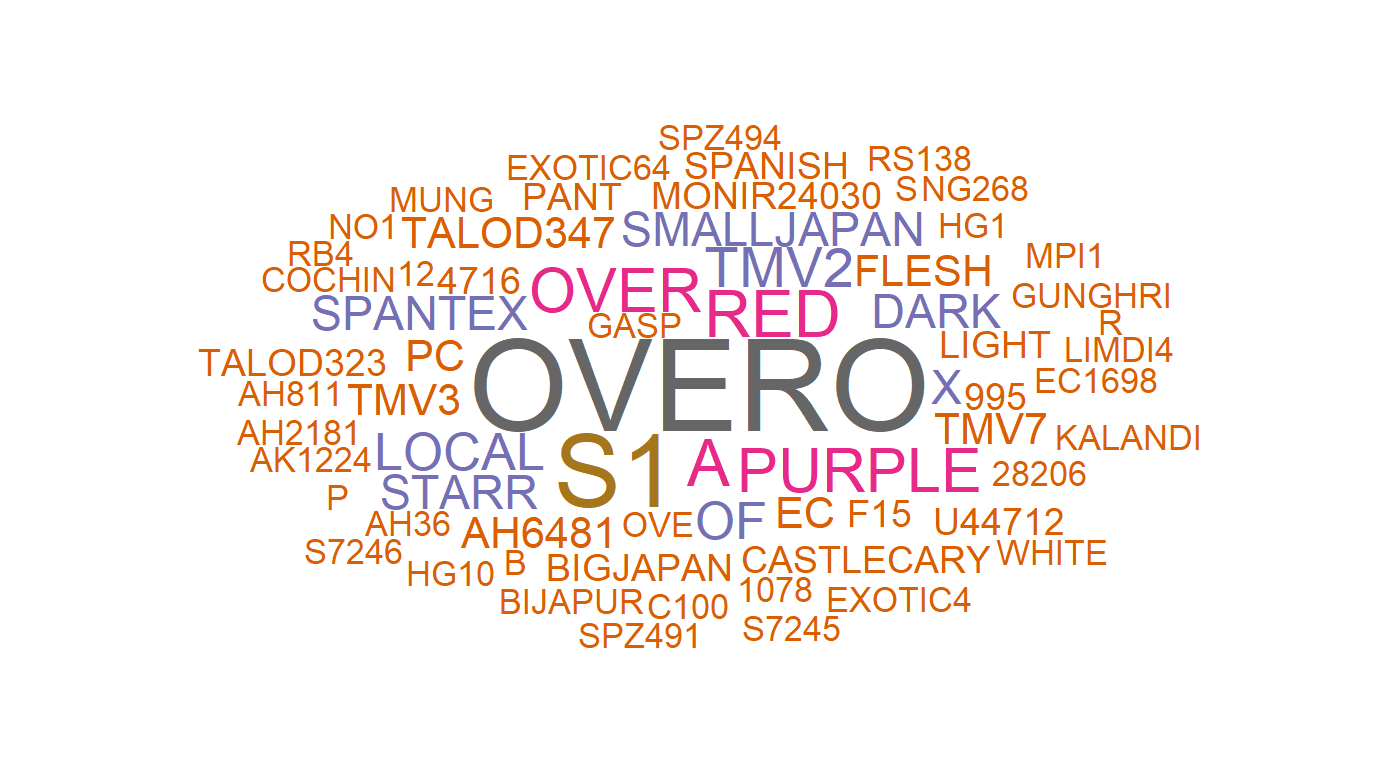
\includegraphics{Introduction_files/figure-latex/unnamed-chunk-23-1.pdf}

\textbf{Fig. 2.} Word cloud of keywords retrieved

The function will throw an error in case of duplicates or NULL values in
the primary key/ID field mentioned.

\begin{Shaded}
\begin{Highlighting}[]
\NormalTok{GN <-}\StringTok{ }\NormalTok{GN1000}
\NormalTok{GN[GNfields] <-}\StringTok{ }\KeywordTok{lapply}\NormalTok{(GN[GNfields], }\ControlFlowTok{function}\NormalTok{(x) }\KeywordTok{DataClean}\NormalTok{(x))}
\CommentTok{# Generate dummy duplicates for illustration}
\NormalTok{GN[}\DecValTok{1001}\OperatorTok{:}\DecValTok{1005}\NormalTok{,] <-}\StringTok{ }\NormalTok{GN[}\DecValTok{1}\OperatorTok{:}\DecValTok{5}\NormalTok{,]}
\CommentTok{# Generate dummy NULL values for illustration}
\NormalTok{GN[}\DecValTok{1001}\NormalTok{,}\DecValTok{3}\NormalTok{] <-}\StringTok{ ""}
\NormalTok{GN[}\DecValTok{1002}\NormalTok{,}\DecValTok{3}\NormalTok{] <-}\StringTok{ ""}
\NormalTok{GN[}\DecValTok{1001}\OperatorTok{:}\DecValTok{1005}\NormalTok{,]}
\end{Highlighting}
\end{Shaded}

\begin{verbatim}
     CommonName    BotanicalName NationalID              CollNo DonorID OtherID1 OtherID2 BioStatus
1001  Groundnut Arachis hypogaea            SHULAMITH NRCG14555 ICG4709            U44712  Landrace
1002  Groundnut Arachis hypogaea                             NC ICG5288      NCS      NC5  Landrace
1003  Groundnut Arachis hypogaea   EC100281             MALIMBA ICG5289          EC100281  Landrace
1004  Groundnut Arachis hypogaea   EC100713            EC100713 ICG5296             STARR  Landrace
1005  Groundnut Arachis hypogaea   EC100715            EC100715 ICG5298             COMET  Landrace
                SourceCountry TransferYear
1001                   Israel         2014
1002 United States of America         2004
1003                   Malawi         2004
1004 United States of America         2004
1005 United States of America         2004
\end{verbatim}

\begin{Shaded}
\begin{Highlighting}[]
\NormalTok{GNKWIC <-}\StringTok{ }\KeywordTok{KWIC}\NormalTok{(GN, GNfields, }\DataTypeTok{min.freq=}\DecValTok{1}\NormalTok{)}
\end{Highlighting}
\end{Shaded}

\begin{verbatim}
Error in KWIC(GN, GNfields, min.freq = 1) :
  Primary key/ID field should be unique and not NULL
 Use PGRdup::ValidatePrimKey() to identify and rectify the aberrant records first
\end{verbatim}

The erroneous records can be identified using the helper function
\texttt{ValidatePrimKey}.

\begin{Shaded}
\begin{Highlighting}[]
\CommentTok{# Validate the primary key/ID field for duplication or existence of NULL values}
\KeywordTok{ValidatePrimKey}\NormalTok{(}\DataTypeTok{x =}\NormalTok{ GN, }\DataTypeTok{prim.key =} \StringTok{"NationalID"}\NormalTok{)}
\end{Highlighting}
\end{Shaded}

\begin{verbatim}
$message1
[1] "ERROR: Duplicated records found in prim.key field"

$Duplicates
     CommonName    BotanicalName NationalID              CollNo DonorID OtherID1 OtherID2 BioStatus
1001  Groundnut Arachis hypogaea            SHULAMITH NRCG14555 ICG4709            U44712  Landrace
1002  Groundnut Arachis hypogaea                             NC ICG5288      NCS      NC5  Landrace
3     Groundnut Arachis hypogaea   EC100281             MALIMBA ICG5289          EC100281  Landrace
1003  Groundnut Arachis hypogaea   EC100281             MALIMBA ICG5289          EC100281  Landrace
4     Groundnut Arachis hypogaea   EC100713            EC100713 ICG5296             STARR  Landrace
1004  Groundnut Arachis hypogaea   EC100713            EC100713 ICG5296             STARR  Landrace
5     Groundnut Arachis hypogaea   EC100715            EC100715 ICG5298             COMET  Landrace
1005  Groundnut Arachis hypogaea   EC100715            EC100715 ICG5298             COMET  Landrace
                SourceCountry TransferYear
1001                   Israel         2014
1002 United States of America         2004
3                      Malawi         2004
1003                   Malawi         2004
4    United States of America         2004
1004 United States of America         2004
5    United States of America         2004
1005 United States of America         2004

$message2
[1] "ERROR: NULL records found in prim.key field"

$NullRecords
     CommonName    BotanicalName NationalID              CollNo DonorID OtherID1 OtherID2 BioStatus
1001  Groundnut Arachis hypogaea            SHULAMITH NRCG14555 ICG4709            U44712  Landrace
1002  Groundnut Arachis hypogaea                             NC ICG5288      NCS      NC5  Landrace
                SourceCountry TransferYear primdup
1001                   Israel         2014    TRUE
1002 United States of America         2004    TRUE
\end{verbatim}

\begin{Shaded}
\begin{Highlighting}[]
\CommentTok{# Remove the offending records}
\NormalTok{GN <-}\StringTok{ }\NormalTok{GN[}\OperatorTok{-}\KeywordTok{c}\NormalTok{(}\DecValTok{1001}\OperatorTok{:}\DecValTok{1005}\NormalTok{), ]}
\CommentTok{# Validate again}
\KeywordTok{ValidatePrimKey}\NormalTok{(}\DataTypeTok{x =}\NormalTok{ GN, }\DataTypeTok{prim.key =} \StringTok{"NationalID"}\NormalTok{)}
\end{Highlighting}
\end{Shaded}

\begin{verbatim}
$message1
[1] "OK: No duplicated records found in prim.key field"

$Duplicates
NULL

$message2
[1] "OK: No NULL records found in prim.key field"

$NullRecords
NULL
\end{verbatim}

\hypertarget{retrieval-of-probable-duplicate-sets}{%
\subsection{Retrieval of Probable Duplicate
Sets}\label{retrieval-of-probable-duplicate-sets}}

Once KWIC indexes are generated, probable duplicates of germplasm
accessions can be identified by fuzzy, phonetic and semantic matching of
the associated keywords using the function \texttt{ProbDup}. The sets
are retrieved as a list of data frames of class \texttt{ProbDup}.

Keywords that are not to be used for matching can be specified as a
vector in the \texttt{excep} argument.

\hypertarget{methods}{%
\subsubsection{Methods}\label{methods}}

The function can execute matching according to either one of the
following three methods as specified by the \texttt{method} argument.

\begin{enumerate}
\def\labelenumi{\arabic{enumi}.}
\tightlist
\item
  \textbf{Method \texttt{"a"}} : Performs string matching of keywords in
  a single KWIC index to identify probable duplicates of accessions in a
  single PGR passport database.
\end{enumerate}

\begin{Shaded}
\begin{Highlighting}[]
\CommentTok{# Load example dataset}
\NormalTok{GN <-}\StringTok{ }\NormalTok{GN1000}

\CommentTok{# Specify as a vector the database fields to be used}
\NormalTok{GNfields <-}\StringTok{ }\KeywordTok{c}\NormalTok{(}\StringTok{"NationalID"}\NormalTok{, }\StringTok{"CollNo"}\NormalTok{, }\StringTok{"DonorID"}\NormalTok{, }\StringTok{"OtherID1"}\NormalTok{, }\StringTok{"OtherID2"}\NormalTok{)}

\CommentTok{# Clean the data}
\NormalTok{GN[GNfields] <-}\StringTok{ }\KeywordTok{lapply}\NormalTok{(GN[GNfields], }\ControlFlowTok{function}\NormalTok{(x) }\KeywordTok{DataClean}\NormalTok{(x))}
\NormalTok{y1 <-}\StringTok{ }\KeywordTok{list}\NormalTok{(}\KeywordTok{c}\NormalTok{(}\StringTok{"Gujarat"}\NormalTok{, }\StringTok{"Dwarf"}\NormalTok{), }\KeywordTok{c}\NormalTok{(}\StringTok{"Castle"}\NormalTok{, }\StringTok{"Cary"}\NormalTok{), }\KeywordTok{c}\NormalTok{(}\StringTok{"Small"}\NormalTok{, }\StringTok{"Japan"}\NormalTok{),}
\KeywordTok{c}\NormalTok{(}\StringTok{"Big"}\NormalTok{, }\StringTok{"Japan"}\NormalTok{), }\KeywordTok{c}\NormalTok{(}\StringTok{"Mani"}\NormalTok{, }\StringTok{"Blanco"}\NormalTok{), }\KeywordTok{c}\NormalTok{(}\StringTok{"Uganda"}\NormalTok{, }\StringTok{"Erect"}\NormalTok{),}
\KeywordTok{c}\NormalTok{(}\StringTok{"Mota"}\NormalTok{, }\StringTok{"Company"}\NormalTok{))}
\NormalTok{y2 <-}\StringTok{ }\KeywordTok{c}\NormalTok{(}\StringTok{"Dark"}\NormalTok{, }\StringTok{"Light"}\NormalTok{, }\StringTok{"Small"}\NormalTok{, }\StringTok{"Improved"}\NormalTok{, }\StringTok{"Punjab"}\NormalTok{, }\StringTok{"SAM"}\NormalTok{)}
\NormalTok{y3 <-}\StringTok{ }\KeywordTok{c}\NormalTok{(}\StringTok{"Local"}\NormalTok{, }\StringTok{"Bold"}\NormalTok{, }\StringTok{"Cary"}\NormalTok{, }\StringTok{"Mutant"}\NormalTok{, }\StringTok{"Runner"}\NormalTok{, }\StringTok{"Giant"}\NormalTok{, }\StringTok{"No."}\NormalTok{,}
        \StringTok{"Bunch"}\NormalTok{, }\StringTok{"Peanut"}\NormalTok{)}
\NormalTok{GN[GNfields] <-}\StringTok{ }\KeywordTok{lapply}\NormalTok{(GN[GNfields],}
                       \ControlFlowTok{function}\NormalTok{(x) }\KeywordTok{MergeKW}\NormalTok{(x, y1, }\DataTypeTok{delim =} \KeywordTok{c}\NormalTok{(}\StringTok{"space"}\NormalTok{, }\StringTok{"dash"}\NormalTok{)))}
\NormalTok{GN[GNfields] <-}\StringTok{ }\KeywordTok{lapply}\NormalTok{(GN[GNfields],}
                       \ControlFlowTok{function}\NormalTok{(x) }\KeywordTok{MergePrefix}\NormalTok{(x, y2, }\DataTypeTok{delim =} \KeywordTok{c}\NormalTok{(}\StringTok{"space"}\NormalTok{, }\StringTok{"dash"}\NormalTok{)))}
\NormalTok{GN[GNfields] <-}\StringTok{ }\KeywordTok{lapply}\NormalTok{(GN[GNfields],}
                       \ControlFlowTok{function}\NormalTok{(x) }\KeywordTok{MergeSuffix}\NormalTok{(x, y3, }\DataTypeTok{delim =} \KeywordTok{c}\NormalTok{(}\StringTok{"space"}\NormalTok{, }\StringTok{"dash"}\NormalTok{)))}

\CommentTok{# Generate the KWIC index}
\NormalTok{GNKWIC <-}\StringTok{ }\KeywordTok{KWIC}\NormalTok{(GN, GNfields)}
\end{Highlighting}
\end{Shaded}

\begin{Shaded}
\begin{Highlighting}[]
\CommentTok{# Specify the exceptions as a vector}
\NormalTok{exep <-}\StringTok{ }\KeywordTok{c}\NormalTok{(}\StringTok{"A"}\NormalTok{, }\StringTok{"B"}\NormalTok{, }\StringTok{"BIG"}\NormalTok{, }\StringTok{"BOLD"}\NormalTok{, }\StringTok{"BUNCH"}\NormalTok{, }\StringTok{"C"}\NormalTok{, }\StringTok{"COMPANY"}\NormalTok{, }\StringTok{"CULTURE"}\NormalTok{,}
         \StringTok{"DARK"}\NormalTok{, }\StringTok{"E"}\NormalTok{, }\StringTok{"EARLY"}\NormalTok{, }\StringTok{"EC"}\NormalTok{, }\StringTok{"ERECT"}\NormalTok{, }\StringTok{"EXOTIC"}\NormalTok{, }\StringTok{"FLESH"}\NormalTok{, }\StringTok{"GROUNDNUT"}\NormalTok{,}
         \StringTok{"GUTHUKAI"}\NormalTok{, }\StringTok{"IMPROVED"}\NormalTok{, }\StringTok{"K"}\NormalTok{, }\StringTok{"KUTHUKADAL"}\NormalTok{, }\StringTok{"KUTHUKAI"}\NormalTok{, }\StringTok{"LARGE"}\NormalTok{,}
         \StringTok{"LIGHT"}\NormalTok{, }\StringTok{"LOCAL"}\NormalTok{, }\StringTok{"OF"}\NormalTok{, }\StringTok{"OVERO"}\NormalTok{, }\StringTok{"P"}\NormalTok{, }\StringTok{"PEANUT"}\NormalTok{, }\StringTok{"PURPLE"}\NormalTok{, }\StringTok{"R"}\NormalTok{,}
         \StringTok{"RED"}\NormalTok{, }\StringTok{"RUNNER"}\NormalTok{, }\StringTok{"S1"}\NormalTok{, }\StringTok{"SAM"}\NormalTok{, }\StringTok{"SMALL"}\NormalTok{, }\StringTok{"SPANISH"}\NormalTok{, }\StringTok{"TAN"}\NormalTok{, }\StringTok{"TYPE"}\NormalTok{,}
         \StringTok{"U"}\NormalTok{, }\StringTok{"VALENCIA"}\NormalTok{, }\StringTok{"VIRGINIA"}\NormalTok{, }\StringTok{"WHITE"}\NormalTok{)}

\CommentTok{# Fetch fuzzy duplicates by method 'a'}
\NormalTok{GNdup <-}\StringTok{ }\KeywordTok{ProbDup}\NormalTok{(}\DataTypeTok{kwic1 =}\NormalTok{ GNKWIC, }\DataTypeTok{method =} \StringTok{"a"}\NormalTok{, }\DataTypeTok{excep =}\NormalTok{ exep, }\DataTypeTok{fuzzy =} \OtherTok{TRUE}\NormalTok{,}
                 \DataTypeTok{phonetic =} \OtherTok{FALSE}\NormalTok{, }\DataTypeTok{semantic =} \OtherTok{FALSE}\NormalTok{)}
\end{Highlighting}
\end{Shaded}

\begin{verbatim}
Fuzzy matching
\end{verbatim}

\begin{verbatim}
  |                                                                                                                       |============================                                                                                   |  25%Block 1 / 4 |  |                                                                                                                       |========================================================                                                       |  50%Block 2 / 4 |  |                                                                                                                       |===================================================================================                            |  75%Block 3 / 4 |  |                                                                                                                       |===============================================================================================================| 100%Block 4 / 4 |
\end{verbatim}

\begin{Shaded}
\begin{Highlighting}[]
\KeywordTok{class}\NormalTok{(GNdup)}
\end{Highlighting}
\end{Shaded}

\begin{verbatim}
[1] "ProbDup"
\end{verbatim}

\begin{Shaded}
\begin{Highlighting}[]
\NormalTok{GNdup}
\end{Highlighting}
\end{Shaded}

\begin{verbatim}
Method : a

KWIC1 fields : NationalID CollNo DonorID OtherID1 OtherID2
 
                No..of.Sets    No..of.Records
FuzzyDuplicates         378               745
Total                   378 745(Distinct:745)
\end{verbatim}

\begin{Shaded}
\begin{Highlighting}[]
\CommentTok{# Fetch phonetic duplicates by method 'a'}
\NormalTok{GNdup <-}\StringTok{ }\KeywordTok{ProbDup}\NormalTok{(}\DataTypeTok{kwic1 =}\NormalTok{ GNKWIC, }\DataTypeTok{method =} \StringTok{"a"}\NormalTok{, }\DataTypeTok{excep =}\NormalTok{ exep, }\DataTypeTok{fuzzy =} \OtherTok{FALSE}\NormalTok{,}
                 \DataTypeTok{phonetic =} \OtherTok{TRUE}\NormalTok{, }\DataTypeTok{semantic =} \OtherTok{FALSE}\NormalTok{)}
\end{Highlighting}
\end{Shaded}

\begin{verbatim}
Phonetic matching
\end{verbatim}

\begin{verbatim}
  |                                                                                                                       |============================                                                                                   |  25%Block 1 / 4 |  |                                                                                                                       |========================================================                                                       |  50%Block 2 / 4 |  |                                                                                                                       |===================================================================================                            |  75%Block 3 / 4 |  |                                                                                                                       |===============================================================================================================| 100%Block 4 / 4 |
\end{verbatim}

\begin{Shaded}
\begin{Highlighting}[]
\KeywordTok{class}\NormalTok{(GNdup)}
\end{Highlighting}
\end{Shaded}

\begin{verbatim}
[1] "ProbDup"
\end{verbatim}

\begin{Shaded}
\begin{Highlighting}[]
\NormalTok{GNdup}
\end{Highlighting}
\end{Shaded}

\begin{verbatim}
Method : a

KWIC1 fields : NationalID CollNo DonorID OtherID1 OtherID2
 
                   No..of.Sets    No..of.Records
PhoneticDuplicates          99               260
Total                       99 260(Distinct:260)
\end{verbatim}

\begin{enumerate}
\def\labelenumi{\arabic{enumi}.}
\setcounter{enumi}{1}
\item
  \textbf{Method \texttt{"b"}} : Performs string matching of keywords in
  the first KWIC index (query) with that of the keywords in the second
  index (source) to identify probable duplicates of accessions of the
  first PGR passport database among the accessions in the second
  database.
\item
  \textbf{Method \texttt{"c"}} : Performs string matching of keywords in
  two different KWIC indexes jointly to identify probable duplicates of
  accessions from among two PGR passport databases.
\end{enumerate}

\begin{Shaded}
\begin{Highlighting}[]
\CommentTok{# Load PGR passport databases}
\NormalTok{GN1 <-}\StringTok{ }\NormalTok{GN1000[}\OperatorTok{!}\KeywordTok{grepl}\NormalTok{(}\StringTok{"^ICG"}\NormalTok{, GN1000}\OperatorTok{$}\NormalTok{DonorID), ]}
\NormalTok{GN1}\OperatorTok{$}\NormalTok{DonorID <-}\StringTok{ }\OtherTok{NULL}
\NormalTok{GN2 <-}\StringTok{ }\NormalTok{GN1000[}\KeywordTok{grepl}\NormalTok{(}\StringTok{"^ICG"}\NormalTok{, GN1000}\OperatorTok{$}\NormalTok{DonorID), ]}
\NormalTok{GN2}\OperatorTok{$}\NormalTok{NationalID <-}\StringTok{ }\OtherTok{NULL}

\CommentTok{# Specify database fields to use}
\NormalTok{GN1fields <-}\StringTok{ }\KeywordTok{c}\NormalTok{(}\StringTok{"NationalID"}\NormalTok{, }\StringTok{"CollNo"}\NormalTok{, }\StringTok{"OtherID1"}\NormalTok{, }\StringTok{"OtherID2"}\NormalTok{)}
\NormalTok{GN2fields <-}\StringTok{ }\KeywordTok{c}\NormalTok{(}\StringTok{"DonorID"}\NormalTok{, }\StringTok{"CollNo"}\NormalTok{, }\StringTok{"OtherID1"}\NormalTok{, }\StringTok{"OtherID2"}\NormalTok{)}

\CommentTok{# Clean the data}
\NormalTok{GN1[GN1fields] <-}\StringTok{ }\KeywordTok{lapply}\NormalTok{(GN1[GN1fields], }\ControlFlowTok{function}\NormalTok{(x) }\KeywordTok{DataClean}\NormalTok{(x))}
\NormalTok{GN2[GN2fields] <-}\StringTok{ }\KeywordTok{lapply}\NormalTok{(GN2[GN2fields], }\ControlFlowTok{function}\NormalTok{(x) }\KeywordTok{DataClean}\NormalTok{(x))}
\NormalTok{y1 <-}\StringTok{ }\KeywordTok{list}\NormalTok{(}\KeywordTok{c}\NormalTok{(}\StringTok{"Gujarat"}\NormalTok{, }\StringTok{"Dwarf"}\NormalTok{), }\KeywordTok{c}\NormalTok{(}\StringTok{"Castle"}\NormalTok{, }\StringTok{"Cary"}\NormalTok{), }\KeywordTok{c}\NormalTok{(}\StringTok{"Small"}\NormalTok{, }\StringTok{"Japan"}\NormalTok{),}
\KeywordTok{c}\NormalTok{(}\StringTok{"Big"}\NormalTok{, }\StringTok{"Japan"}\NormalTok{), }\KeywordTok{c}\NormalTok{(}\StringTok{"Mani"}\NormalTok{, }\StringTok{"Blanco"}\NormalTok{), }\KeywordTok{c}\NormalTok{(}\StringTok{"Uganda"}\NormalTok{, }\StringTok{"Erect"}\NormalTok{),}
\KeywordTok{c}\NormalTok{(}\StringTok{"Mota"}\NormalTok{, }\StringTok{"Company"}\NormalTok{))}
\NormalTok{y2 <-}\StringTok{ }\KeywordTok{c}\NormalTok{(}\StringTok{"Dark"}\NormalTok{, }\StringTok{"Light"}\NormalTok{, }\StringTok{"Small"}\NormalTok{, }\StringTok{"Improved"}\NormalTok{, }\StringTok{"Punjab"}\NormalTok{, }\StringTok{"SAM"}\NormalTok{)}
\NormalTok{y3 <-}\StringTok{ }\KeywordTok{c}\NormalTok{(}\StringTok{"Local"}\NormalTok{, }\StringTok{"Bold"}\NormalTok{, }\StringTok{"Cary"}\NormalTok{, }\StringTok{"Mutant"}\NormalTok{, }\StringTok{"Runner"}\NormalTok{, }\StringTok{"Giant"}\NormalTok{, }\StringTok{"No."}\NormalTok{,}
        \StringTok{"Bunch"}\NormalTok{, }\StringTok{"Peanut"}\NormalTok{)}
\NormalTok{GN1[GN1fields] <-}\StringTok{ }\KeywordTok{lapply}\NormalTok{(GN1[GN1fields],}
                         \ControlFlowTok{function}\NormalTok{(x) }\KeywordTok{MergeKW}\NormalTok{(x, y1, }\DataTypeTok{delim =} \KeywordTok{c}\NormalTok{(}\StringTok{"space"}\NormalTok{, }\StringTok{"dash"}\NormalTok{)))}
\NormalTok{GN1[GN1fields] <-}\StringTok{ }\KeywordTok{lapply}\NormalTok{(GN1[GN1fields],}
                         \ControlFlowTok{function}\NormalTok{(x) }\KeywordTok{MergePrefix}\NormalTok{(x, y2, }\DataTypeTok{delim =} \KeywordTok{c}\NormalTok{(}\StringTok{"space"}\NormalTok{, }\StringTok{"dash"}\NormalTok{)))}
\NormalTok{GN1[GN1fields] <-}\StringTok{ }\KeywordTok{lapply}\NormalTok{(GN1[GN1fields],}
                         \ControlFlowTok{function}\NormalTok{(x) }\KeywordTok{MergeSuffix}\NormalTok{(x, y3, }\DataTypeTok{delim =} \KeywordTok{c}\NormalTok{(}\StringTok{"space"}\NormalTok{, }\StringTok{"dash"}\NormalTok{)))}
\NormalTok{GN2[GN2fields] <-}\StringTok{ }\KeywordTok{lapply}\NormalTok{(GN2[GN2fields],}
                         \ControlFlowTok{function}\NormalTok{(x) }\KeywordTok{MergeKW}\NormalTok{(x, y1, }\DataTypeTok{delim =} \KeywordTok{c}\NormalTok{(}\StringTok{"space"}\NormalTok{, }\StringTok{"dash"}\NormalTok{)))}
\NormalTok{GN2[GN2fields] <-}\StringTok{ }\KeywordTok{lapply}\NormalTok{(GN2[GN2fields],}
                         \ControlFlowTok{function}\NormalTok{(x) }\KeywordTok{MergePrefix}\NormalTok{(x, y2, }\DataTypeTok{delim =} \KeywordTok{c}\NormalTok{(}\StringTok{"space"}\NormalTok{, }\StringTok{"dash"}\NormalTok{)))}
\NormalTok{GN2[GN2fields] <-}\StringTok{ }\KeywordTok{lapply}\NormalTok{(GN2[GN2fields],}
                         \ControlFlowTok{function}\NormalTok{(x) }\KeywordTok{MergeSuffix}\NormalTok{(x, y3, }\DataTypeTok{delim =} \KeywordTok{c}\NormalTok{(}\StringTok{"space"}\NormalTok{, }\StringTok{"dash"}\NormalTok{)))}

\CommentTok{# Remove duplicated DonorID records in GN2}
\NormalTok{GN2 <-}\StringTok{ }\NormalTok{GN2[}\OperatorTok{!}\KeywordTok{duplicated}\NormalTok{(GN2}\OperatorTok{$}\NormalTok{DonorID), ]}

\CommentTok{# Generate KWIC index}
\NormalTok{GN1KWIC <-}\StringTok{ }\KeywordTok{KWIC}\NormalTok{(GN1, GN1fields)}
\NormalTok{GN2KWIC <-}\StringTok{ }\KeywordTok{KWIC}\NormalTok{(GN2, GN2fields)}

\CommentTok{# Specify the exceptions as a vector}
\NormalTok{exep <-}\StringTok{ }\KeywordTok{c}\NormalTok{(}\StringTok{"A"}\NormalTok{, }\StringTok{"B"}\NormalTok{, }\StringTok{"BIG"}\NormalTok{, }\StringTok{"BOLD"}\NormalTok{, }\StringTok{"BUNCH"}\NormalTok{, }\StringTok{"C"}\NormalTok{, }\StringTok{"COMPANY"}\NormalTok{, }\StringTok{"CULTURE"}\NormalTok{,}
         \StringTok{"DARK"}\NormalTok{, }\StringTok{"E"}\NormalTok{, }\StringTok{"EARLY"}\NormalTok{, }\StringTok{"EC"}\NormalTok{, }\StringTok{"ERECT"}\NormalTok{, }\StringTok{"EXOTIC"}\NormalTok{, }\StringTok{"FLESH"}\NormalTok{, }\StringTok{"GROUNDNUT"}\NormalTok{,}
         \StringTok{"GUTHUKAI"}\NormalTok{, }\StringTok{"IMPROVED"}\NormalTok{, }\StringTok{"K"}\NormalTok{, }\StringTok{"KUTHUKADAL"}\NormalTok{, }\StringTok{"KUTHUKAI"}\NormalTok{, }\StringTok{"LARGE"}\NormalTok{,}
         \StringTok{"LIGHT"}\NormalTok{, }\StringTok{"LOCAL"}\NormalTok{, }\StringTok{"OF"}\NormalTok{, }\StringTok{"OVERO"}\NormalTok{, }\StringTok{"P"}\NormalTok{, }\StringTok{"PEANUT"}\NormalTok{, }\StringTok{"PURPLE"}\NormalTok{, }\StringTok{"R"}\NormalTok{,}
         \StringTok{"RED"}\NormalTok{, }\StringTok{"RUNNER"}\NormalTok{, }\StringTok{"S1"}\NormalTok{, }\StringTok{"SAM"}\NormalTok{, }\StringTok{"SMALL"}\NormalTok{, }\StringTok{"SPANISH"}\NormalTok{, }\StringTok{"TAN"}\NormalTok{, }\StringTok{"TYPE"}\NormalTok{,}
         \StringTok{"U"}\NormalTok{, }\StringTok{"VALENCIA"}\NormalTok{, }\StringTok{"VIRGINIA"}\NormalTok{, }\StringTok{"WHITE"}\NormalTok{)}

\CommentTok{# Fetch fuzzy and phonetic duplicate sets by method b}
\NormalTok{GNdupb <-}\StringTok{ }\KeywordTok{ProbDup}\NormalTok{(}\DataTypeTok{kwic1 =}\NormalTok{ GN1KWIC, }\DataTypeTok{kwic2 =}\NormalTok{ GN2KWIC, }\DataTypeTok{method =} \StringTok{"b"}\NormalTok{,}
                  \DataTypeTok{excep =}\NormalTok{ exep, }\DataTypeTok{fuzzy =} \OtherTok{TRUE}\NormalTok{, }\DataTypeTok{phonetic =} \OtherTok{TRUE}\NormalTok{,}
                  \DataTypeTok{encoding =} \StringTok{"primary"}\NormalTok{, }\DataTypeTok{semantic =} \OtherTok{FALSE}\NormalTok{)}
\end{Highlighting}
\end{Shaded}

\begin{verbatim}
Fuzzy matching
\end{verbatim}

\begin{verbatim}
  |                                                                                                                       |===============================================================================================================| 100%Block 1 / 1 |
\end{verbatim}

\begin{verbatim}
Phonetic matching
\end{verbatim}

\begin{verbatim}
  |                                                                                                                       |===============================================================================================================| 100%Block 1 / 1 |
\end{verbatim}

\begin{Shaded}
\begin{Highlighting}[]
\KeywordTok{class}\NormalTok{(GNdupb)}
\end{Highlighting}
\end{Shaded}

\begin{verbatim}
[1] "ProbDup"
\end{verbatim}

\begin{Shaded}
\begin{Highlighting}[]
\NormalTok{GNdupb}
\end{Highlighting}
\end{Shaded}

\begin{verbatim}
Method : b

KWIC1 fields : NationalID CollNo OtherID1 OtherID2

KWIC2 fields : DonorID CollNo OtherID1 OtherID2
 
                   No..of.Sets    No..of.Records
FuzzyDuplicates            107               353
PhoneticDuplicates          41               126
Total                      148 479(Distinct:383)
\end{verbatim}

\begin{Shaded}
\begin{Highlighting}[]
\CommentTok{# Fetch fuzzy and phonetic duplicate sets by method c}
\NormalTok{GNdupc <-}\StringTok{ }\KeywordTok{ProbDup}\NormalTok{(}\DataTypeTok{kwic1 =}\NormalTok{ GN1KWIC, }\DataTypeTok{kwic2 =}\NormalTok{ GN2KWIC, }\DataTypeTok{method =} \StringTok{"c"}\NormalTok{,}
                  \DataTypeTok{excep =}\NormalTok{ exep, }\DataTypeTok{fuzzy =} \OtherTok{TRUE}\NormalTok{, }\DataTypeTok{phonetic =} \OtherTok{TRUE}\NormalTok{,}
                  \DataTypeTok{encoding =} \StringTok{"primary"}\NormalTok{, }\DataTypeTok{semantic =} \OtherTok{FALSE}\NormalTok{)}
\end{Highlighting}
\end{Shaded}

\begin{verbatim}
Fuzzy matching
\end{verbatim}

\begin{verbatim}
  |                                                                                                                       |=====================================                                                                          |  33%Block 1 / 3 |  |                                                                                                                       |==========================================================================                                     |  67%Block 2 / 3 |  |                                                                                                                       |===============================================================================================================| 100%Block 3 / 3 |
\end{verbatim}

\begin{verbatim}
Phonetic matching
\end{verbatim}

\begin{verbatim}
  |                                                                                                                       |=====================================                                                                          |  33%Block 1 / 3 |  |                                                                                                                       |==========================================================================                                     |  67%Block 2 / 3 |  |                                                                                                                       |===============================================================================================================| 100%Block 3 / 3 |
\end{verbatim}

\begin{Shaded}
\begin{Highlighting}[]
\KeywordTok{class}\NormalTok{(GNdupc)}
\end{Highlighting}
\end{Shaded}

\begin{verbatim}
[1] "ProbDup"
\end{verbatim}

\begin{Shaded}
\begin{Highlighting}[]
\NormalTok{GNdupc}
\end{Highlighting}
\end{Shaded}

\begin{verbatim}
Method : c

KWIC1 fields : NationalID CollNo OtherID1 OtherID2

KWIC2 fields : DonorID CollNo OtherID1 OtherID2
 
                   No..of.Sets    No..of.Records
FuzzyDuplicates            363               724
PhoneticDuplicates          98               257
Total                      461 981(Distinct:741)
\end{verbatim}

\hypertarget{matching-strategies}{%
\subsubsection{Matching Strategies}\label{matching-strategies}}

\begin{enumerate}
\def\labelenumi{\arabic{enumi}.}
\tightlist
\item
  \textbf{Fuzzy matching} or approximate string matching of keywords is
  carried out by computing the
  \href{https://en.wikipedia.org/wiki/Levenshtein_distance}{generalized
  levenshtein (edit) distance} between them. This distance measure
  counts the number of deletions, insertions and substitutions necessary
  to turn one string to another.
\end{enumerate}

\begin{Shaded}
\begin{Highlighting}[]
\CommentTok{# Load example dataset}
\NormalTok{GN <-}\StringTok{ }\NormalTok{GN1000}

\CommentTok{# Specify as a vector the database fields to be used}
\NormalTok{GNfields <-}\StringTok{ }\KeywordTok{c}\NormalTok{(}\StringTok{"NationalID"}\NormalTok{, }\StringTok{"CollNo"}\NormalTok{, }\StringTok{"DonorID"}\NormalTok{, }\StringTok{"OtherID1"}\NormalTok{, }\StringTok{"OtherID2"}\NormalTok{)}

\CommentTok{# Clean the data}
\NormalTok{GN[GNfields] <-}\StringTok{ }\KeywordTok{lapply}\NormalTok{(GN[GNfields], }\ControlFlowTok{function}\NormalTok{(x) }\KeywordTok{DataClean}\NormalTok{(x))}
\NormalTok{y1 <-}\StringTok{ }\KeywordTok{list}\NormalTok{(}\KeywordTok{c}\NormalTok{(}\StringTok{"Gujarat"}\NormalTok{, }\StringTok{"Dwarf"}\NormalTok{), }\KeywordTok{c}\NormalTok{(}\StringTok{"Castle"}\NormalTok{, }\StringTok{"Cary"}\NormalTok{), }\KeywordTok{c}\NormalTok{(}\StringTok{"Small"}\NormalTok{, }\StringTok{"Japan"}\NormalTok{),}
\KeywordTok{c}\NormalTok{(}\StringTok{"Big"}\NormalTok{, }\StringTok{"Japan"}\NormalTok{), }\KeywordTok{c}\NormalTok{(}\StringTok{"Mani"}\NormalTok{, }\StringTok{"Blanco"}\NormalTok{), }\KeywordTok{c}\NormalTok{(}\StringTok{"Uganda"}\NormalTok{, }\StringTok{"Erect"}\NormalTok{),}
\KeywordTok{c}\NormalTok{(}\StringTok{"Mota"}\NormalTok{, }\StringTok{"Company"}\NormalTok{))}
\NormalTok{y2 <-}\StringTok{ }\KeywordTok{c}\NormalTok{(}\StringTok{"Dark"}\NormalTok{, }\StringTok{"Light"}\NormalTok{, }\StringTok{"Small"}\NormalTok{, }\StringTok{"Improved"}\NormalTok{, }\StringTok{"Punjab"}\NormalTok{, }\StringTok{"SAM"}\NormalTok{)}
\NormalTok{y3 <-}\StringTok{ }\KeywordTok{c}\NormalTok{(}\StringTok{"Local"}\NormalTok{, }\StringTok{"Bold"}\NormalTok{, }\StringTok{"Cary"}\NormalTok{, }\StringTok{"Mutant"}\NormalTok{, }\StringTok{"Runner"}\NormalTok{, }\StringTok{"Giant"}\NormalTok{, }\StringTok{"No."}\NormalTok{,}
        \StringTok{"Bunch"}\NormalTok{, }\StringTok{"Peanut"}\NormalTok{)}
\NormalTok{GN[GNfields] <-}\StringTok{ }\KeywordTok{lapply}\NormalTok{(GN[GNfields],}
                       \ControlFlowTok{function}\NormalTok{(x) }\KeywordTok{MergeKW}\NormalTok{(x, y1, }\DataTypeTok{delim =} \KeywordTok{c}\NormalTok{(}\StringTok{"space"}\NormalTok{, }\StringTok{"dash"}\NormalTok{)))}
\NormalTok{GN[GNfields] <-}\StringTok{ }\KeywordTok{lapply}\NormalTok{(GN[GNfields],}
                       \ControlFlowTok{function}\NormalTok{(x) }\KeywordTok{MergePrefix}\NormalTok{(x, y2, }\DataTypeTok{delim =} \KeywordTok{c}\NormalTok{(}\StringTok{"space"}\NormalTok{, }\StringTok{"dash"}\NormalTok{)))}
\NormalTok{GN[GNfields] <-}\StringTok{ }\KeywordTok{lapply}\NormalTok{(GN[GNfields],}
                       \ControlFlowTok{function}\NormalTok{(x) }\KeywordTok{MergeSuffix}\NormalTok{(x, y3, }\DataTypeTok{delim =} \KeywordTok{c}\NormalTok{(}\StringTok{"space"}\NormalTok{, }\StringTok{"dash"}\NormalTok{)))}

\CommentTok{# Generate the KWIC index}
\NormalTok{GNKWIC <-}\StringTok{ }\KeywordTok{KWIC}\NormalTok{(GN, GNfields)}

\CommentTok{# Specify the exceptions as a vector}
\NormalTok{exep <-}\StringTok{ }\KeywordTok{c}\NormalTok{(}\StringTok{"A"}\NormalTok{, }\StringTok{"B"}\NormalTok{, }\StringTok{"BIG"}\NormalTok{, }\StringTok{"BOLD"}\NormalTok{, }\StringTok{"BUNCH"}\NormalTok{, }\StringTok{"C"}\NormalTok{, }\StringTok{"COMPANY"}\NormalTok{, }\StringTok{"CULTURE"}\NormalTok{,}
         \StringTok{"DARK"}\NormalTok{, }\StringTok{"E"}\NormalTok{, }\StringTok{"EARLY"}\NormalTok{, }\StringTok{"EC"}\NormalTok{, }\StringTok{"ERECT"}\NormalTok{, }\StringTok{"EXOTIC"}\NormalTok{, }\StringTok{"FLESH"}\NormalTok{, }\StringTok{"GROUNDNUT"}\NormalTok{,}
         \StringTok{"GUTHUKAI"}\NormalTok{, }\StringTok{"IMPROVED"}\NormalTok{, }\StringTok{"K"}\NormalTok{, }\StringTok{"KUTHUKADAL"}\NormalTok{, }\StringTok{"KUTHUKAI"}\NormalTok{, }\StringTok{"LARGE"}\NormalTok{,}
         \StringTok{"LIGHT"}\NormalTok{, }\StringTok{"LOCAL"}\NormalTok{, }\StringTok{"OF"}\NormalTok{, }\StringTok{"OVERO"}\NormalTok{, }\StringTok{"P"}\NormalTok{, }\StringTok{"PEANUT"}\NormalTok{, }\StringTok{"PURPLE"}\NormalTok{, }\StringTok{"R"}\NormalTok{,}
         \StringTok{"RED"}\NormalTok{, }\StringTok{"RUNNER"}\NormalTok{, }\StringTok{"S1"}\NormalTok{, }\StringTok{"SAM"}\NormalTok{, }\StringTok{"SMALL"}\NormalTok{, }\StringTok{"SPANISH"}\NormalTok{, }\StringTok{"TAN"}\NormalTok{, }\StringTok{"TYPE"}\NormalTok{,}
         \StringTok{"U"}\NormalTok{, }\StringTok{"VALENCIA"}\NormalTok{, }\StringTok{"VIRGINIA"}\NormalTok{, }\StringTok{"WHITE"}\NormalTok{)}

\CommentTok{# Fetch fuzzy duplicates}
\NormalTok{GNdup <-}\StringTok{ }\KeywordTok{ProbDup}\NormalTok{(}\DataTypeTok{kwic1 =}\NormalTok{ GNKWIC, }\DataTypeTok{method =} \StringTok{"a"}\NormalTok{, }\DataTypeTok{excep =}\NormalTok{ exep, }
                 \DataTypeTok{fuzzy =} \OtherTok{TRUE}\NormalTok{, }\DataTypeTok{max.dist =} \DecValTok{3}\NormalTok{,}
                 \DataTypeTok{phonetic =} \OtherTok{FALSE}\NormalTok{, }\DataTypeTok{semantic =} \OtherTok{FALSE}\NormalTok{)}
\end{Highlighting}
\end{Shaded}

\begin{verbatim}
Fuzzy matching
\end{verbatim}

\begin{verbatim}
  |                                                                                                                       |============================                                                                                   |  25%Block 1 / 4 |  |                                                                                                                       |========================================================                                                       |  50%Block 2 / 4 |  |                                                                                                                       |===================================================================================                            |  75%Block 3 / 4 |  |                                                                                                                       |===============================================================================================================| 100%Block 4 / 4 |
\end{verbatim}

\begin{Shaded}
\begin{Highlighting}[]
\NormalTok{GNdup}
\end{Highlighting}
\end{Shaded}

\begin{verbatim}
Method : a

KWIC1 fields : NationalID CollNo DonorID OtherID1 OtherID2
 
                No..of.Sets    No..of.Records
FuzzyDuplicates         378               745
Total                   378 745(Distinct:745)
\end{verbatim}

The maximum distance to be considered for a match can be specified by
\texttt{max.dist} argument.

\begin{Shaded}
\begin{Highlighting}[]
\NormalTok{GNdup <-}\StringTok{ }\KeywordTok{ProbDup}\NormalTok{(}\DataTypeTok{kwic1 =}\NormalTok{ GNKWIC, }\DataTypeTok{method =} \StringTok{"a"}\NormalTok{, }\DataTypeTok{excep =}\NormalTok{ exep, }
                 \DataTypeTok{fuzzy =} \OtherTok{TRUE}\NormalTok{, }\DataTypeTok{max.dist =} \DecValTok{1}\NormalTok{,}
                 \DataTypeTok{phonetic =} \OtherTok{FALSE}\NormalTok{, }\DataTypeTok{semantic =} \OtherTok{FALSE}\NormalTok{)}
\end{Highlighting}
\end{Shaded}

\begin{verbatim}
Fuzzy matching
\end{verbatim}

\begin{verbatim}
  |                                                                                                                       |============================                                                                                   |  25%Block 1 / 4 |  |                                                                                                                       |========================================================                                                       |  50%Block 2 / 4 |  |                                                                                                                       |===================================================================================                            |  75%Block 3 / 4 |  |                                                                                                                       |===============================================================================================================| 100%Block 4 / 4 |
\end{verbatim}

\begin{Shaded}
\begin{Highlighting}[]
\NormalTok{GNdup}
\end{Highlighting}
\end{Shaded}

\begin{verbatim}
Method : a

KWIC1 fields : NationalID CollNo DonorID OtherID1 OtherID2
 
                No..of.Sets    No..of.Records
FuzzyDuplicates         288               679
Total                   288 679(Distinct:679)
\end{verbatim}

Exact matching can be enforced with the argument \texttt{force.exact}
set as TRUE. It can be used to avoid fuzzy matching when the number of
alphabet characters in keywords is lesser than a critical value
(\texttt{max.alpha}). Similarly, the value of \texttt{max.digit} can
also be set according to the requirements to enforce exact matching. The
default value of \texttt{Inf} avoids fuzzy matching and enforces exact
matching for all keywords having any numerical characters. If
\texttt{max.digit} and \texttt{max.alpha} are both set to \texttt{Inf},
exact matching will be enforced for all the keywords.

When exact matching is enforced, for keywords having both alphabet and
numeric characters and with the number of alphabet characters greater
than \texttt{max.digit}, matching will be carried out separately for
alphabet and numeric characters present.

\begin{Shaded}
\begin{Highlighting}[]
\NormalTok{GNdup <-}\StringTok{ }\KeywordTok{ProbDup}\NormalTok{(}\DataTypeTok{kwic1 =}\NormalTok{ GNKWIC, }\DataTypeTok{method =} \StringTok{"a"}\NormalTok{, }\DataTypeTok{excep =}\NormalTok{ exep, }
                 \DataTypeTok{fuzzy =} \OtherTok{TRUE}\NormalTok{, }\DataTypeTok{force.exact =} \OtherTok{TRUE}\NormalTok{, }\DataTypeTok{max.alpha =} \DecValTok{4}\NormalTok{, }\DataTypeTok{max.digit =} \OtherTok{Inf}\NormalTok{,}
                 \DataTypeTok{phonetic =} \OtherTok{FALSE}\NormalTok{, }\DataTypeTok{semantic =} \OtherTok{FALSE}\NormalTok{)}
\end{Highlighting}
\end{Shaded}

\begin{verbatim}
Fuzzy matching
\end{verbatim}

\begin{verbatim}
  |                                                                                                                       |============================                                                                                   |  25%Block 1 / 4 |  |                                                                                                                       |========================================================                                                       |  50%Block 2 / 4 |  |                                                                                                                       |===================================================================================                            |  75%Block 3 / 4 |  |                                                                                                                       |===============================================================================================================| 100%Block 4 / 4 |
\end{verbatim}

\begin{Shaded}
\begin{Highlighting}[]
\NormalTok{GNdup}
\end{Highlighting}
\end{Shaded}

\begin{verbatim}
Method : a

KWIC1 fields : NationalID CollNo DonorID OtherID1 OtherID2
 
                No..of.Sets    No..of.Records
FuzzyDuplicates         378               745
Total                   378 745(Distinct:745)
\end{verbatim}

\begin{enumerate}
\def\labelenumi{\arabic{enumi}.}
\setcounter{enumi}{1}
\tightlist
\item
  \textbf{Phonetic matching} of keywords is carried out using the Double
  Metaphone phonetic algorithm which is implemented as the helper
  function \texttt{DoubleMetaphone}, (Philips
  \protect\hyperlink{ref-p00}{2000}), to identify keywords that have the
  similar pronunciation.
\end{enumerate}

\begin{Shaded}
\begin{Highlighting}[]
\NormalTok{GNdup <-}\StringTok{ }\KeywordTok{ProbDup}\NormalTok{(}\DataTypeTok{kwic1 =}\NormalTok{ GNKWIC, }\DataTypeTok{method =} \StringTok{"a"}\NormalTok{, }\DataTypeTok{excep =}\NormalTok{ exep, }
                 \DataTypeTok{fuzzy =} \OtherTok{FALSE}\NormalTok{,}
                 \DataTypeTok{phonetic =} \OtherTok{TRUE}\NormalTok{,}
                 \DataTypeTok{semantic =} \OtherTok{FALSE}\NormalTok{)}
\end{Highlighting}
\end{Shaded}

\begin{verbatim}
Phonetic matching
\end{verbatim}

\begin{verbatim}
  |                                                                                                                       |============================                                                                                   |  25%Block 1 / 4 |  |                                                                                                                       |========================================================                                                       |  50%Block 2 / 4 |  |                                                                                                                       |===================================================================================                            |  75%Block 3 / 4 |  |                                                                                                                       |===============================================================================================================| 100%Block 4 / 4 |
\end{verbatim}

\begin{Shaded}
\begin{Highlighting}[]
\NormalTok{GNdup}
\end{Highlighting}
\end{Shaded}

\begin{verbatim}
Method : a

KWIC1 fields : NationalID CollNo DonorID OtherID1 OtherID2
 
                   No..of.Sets    No..of.Records
PhoneticDuplicates          99               260
Total                       99 260(Distinct:260)
\end{verbatim}

Either the primary or alternate encodings can be used by specifying the
\texttt{encoding} argument.

\begin{Shaded}
\begin{Highlighting}[]
\NormalTok{GNdup <-}\StringTok{ }\KeywordTok{ProbDup}\NormalTok{(}\DataTypeTok{kwic1 =}\NormalTok{ GNKWIC, }\DataTypeTok{method =} \StringTok{"a"}\NormalTok{, }\DataTypeTok{excep =}\NormalTok{ exep, }
                 \DataTypeTok{fuzzy =} \OtherTok{FALSE}\NormalTok{,}
                 \DataTypeTok{phonetic =} \OtherTok{TRUE}\NormalTok{, }\DataTypeTok{encoding =} \StringTok{"alternate"}\NormalTok{,}
                 \DataTypeTok{semantic =} \OtherTok{FALSE}\NormalTok{)}
\end{Highlighting}
\end{Shaded}

\begin{verbatim}
Phonetic matching
\end{verbatim}

\begin{verbatim}
  |                                                                                                                       |============================                                                                                   |  25%Block 1 / 4 |  |                                                                                                                       |========================================================                                                       |  50%Block 2 / 4 |  |                                                                                                                       |===================================================================================                            |  75%Block 3 / 4 |  |                                                                                                                       |===============================================================================================================| 100%Block 4 / 4 |
\end{verbatim}

\begin{Shaded}
\begin{Highlighting}[]
\NormalTok{GNdup}
\end{Highlighting}
\end{Shaded}

\begin{verbatim}
Method : a

KWIC1 fields : NationalID CollNo DonorID OtherID1 OtherID2
 
                   No..of.Sets    No..of.Records
PhoneticDuplicates          98               263
Total                       98 263(Distinct:263)
\end{verbatim}

The argument \texttt{phon.min.alpha} sets the limits for the number of
alphabet characters to be present in a string for executing phonetic
matching.

\begin{Shaded}
\begin{Highlighting}[]
\NormalTok{GNdup <-}\StringTok{ }\KeywordTok{ProbDup}\NormalTok{(}\DataTypeTok{kwic1 =}\NormalTok{ GNKWIC, }\DataTypeTok{method =} \StringTok{"a"}\NormalTok{, }\DataTypeTok{excep =}\NormalTok{ exep, }
                 \DataTypeTok{fuzzy =} \OtherTok{FALSE}\NormalTok{,}
                 \DataTypeTok{phonetic =} \OtherTok{TRUE}\NormalTok{, }\DataTypeTok{encoding =} \StringTok{"alternate"}\NormalTok{, }\DataTypeTok{phon.min.alpha =} \DecValTok{4}\NormalTok{,}
                 \DataTypeTok{semantic =} \OtherTok{FALSE}\NormalTok{)}
\end{Highlighting}
\end{Shaded}

\begin{verbatim}
Phonetic matching
\end{verbatim}

\begin{verbatim}
  |                                                                                                                       |============================                                                                                   |  25%Block 1 / 4 |  |                                                                                                                       |========================================================                                                       |  50%Block 2 / 4 |  |                                                                                                                       |===================================================================================                            |  75%Block 3 / 4 |  |                                                                                                                       |===============================================================================================================| 100%Block 4 / 4 |
\end{verbatim}

\begin{Shaded}
\begin{Highlighting}[]
\NormalTok{GNdup}
\end{Highlighting}
\end{Shaded}

\begin{verbatim}
Method : a

KWIC1 fields : NationalID CollNo DonorID OtherID1 OtherID2
 
                   No..of.Sets    No..of.Records
PhoneticDuplicates         304               451
Total                      304 451(Distinct:451)
\end{verbatim}

Similarly \texttt{min.enc} sets the limits for the number of characters
to be present in the encoding of a keyword for phonetic matching.

\begin{Shaded}
\begin{Highlighting}[]
\NormalTok{GNdup <-}\StringTok{ }\KeywordTok{ProbDup}\NormalTok{(}\DataTypeTok{kwic1 =}\NormalTok{ GNKWIC, }\DataTypeTok{method =} \StringTok{"a"}\NormalTok{, }\DataTypeTok{excep =}\NormalTok{ exep, }
                 \DataTypeTok{fuzzy =} \OtherTok{FALSE}\NormalTok{,}
                 \DataTypeTok{phonetic =} \OtherTok{TRUE}\NormalTok{, }\DataTypeTok{encoding =} \StringTok{"alternate"}\NormalTok{, }\DataTypeTok{min.enc =} \DecValTok{4}\NormalTok{,}
                 \DataTypeTok{semantic =} \OtherTok{FALSE}\NormalTok{)}
\end{Highlighting}
\end{Shaded}

\begin{verbatim}
Phonetic matching
\end{verbatim}

\begin{verbatim}
  |                                                                                                                       |============================                                                                                   |  25%Block 1 / 4 |  |                                                                                                                       |========================================================                                                       |  50%Block 2 / 4 |  |                                                                                                                       |===================================================================================                            |  75%Block 3 / 4 |  |                                                                                                                       |===============================================================================================================| 100%Block 4 / 4 |
\end{verbatim}

\begin{Shaded}
\begin{Highlighting}[]
\NormalTok{GNdup}
\end{Highlighting}
\end{Shaded}

\begin{verbatim}
Method : a

KWIC1 fields : NationalID CollNo DonorID OtherID1 OtherID2
 
                   No..of.Sets    No..of.Records
PhoneticDuplicates          59               156
Total                       59 156(Distinct:156)
\end{verbatim}

\begin{enumerate}
\def\labelenumi{\arabic{enumi}.}
\setcounter{enumi}{2}
\tightlist
\item
  \textbf{Semantic matching} matches keywords based on a list of
  accession name synonyms supplied as list with character vectors of
  synonym sets (synsets) to the \texttt{syn} argument. Synonyms in this
  context refer to interchangeable identifiers or names by which an
  accession is recognized. Multiple keywords specified as members of the
  same synset in \texttt{syn} are matched. To facilitate accurate
  identification of synonyms from the KWIC index, identical data
  standardization operations using the \texttt{Merge*} and
  \texttt{DataClean} functions for both the original database fields and
  the synset list are recommended.
\end{enumerate}

\begin{Shaded}
\begin{Highlighting}[]
\CommentTok{# Specify the synsets as a list}
\NormalTok{syn <-}\StringTok{ }\KeywordTok{list}\NormalTok{(}\KeywordTok{c}\NormalTok{(}\StringTok{"CHANDRA"}\NormalTok{, }\StringTok{"AH 114"}\NormalTok{), }\KeywordTok{c}\NormalTok{(}\StringTok{"TG-1"}\NormalTok{, }\StringTok{"VIKRAM"}\NormalTok{))}

\CommentTok{# Clean the data in the synsets}
\NormalTok{syn <-}\StringTok{ }\KeywordTok{lapply}\NormalTok{(syn, DataClean)}

\NormalTok{GNdup <-}\StringTok{ }\KeywordTok{ProbDup}\NormalTok{(}\DataTypeTok{kwic1 =}\NormalTok{ GNKWIC, }\DataTypeTok{method =} \StringTok{"a"}\NormalTok{, }\DataTypeTok{excep =}\NormalTok{ exep, }
                 \DataTypeTok{fuzzy =} \OtherTok{FALSE}\NormalTok{, }\DataTypeTok{phonetic =} \OtherTok{FALSE}\NormalTok{,}
                 \DataTypeTok{semantic =} \OtherTok{TRUE}\NormalTok{, }\DataTypeTok{syn =}\NormalTok{ syn)}
\end{Highlighting}
\end{Shaded}

\begin{verbatim}
Semantic matching
\end{verbatim}

\begin{verbatim}
  |                                                                                                                       |============================                                                                                   |  25%Block 1 / 4 |  |                                                                                                                       |========================================================                                                       |  50%Block 2 / 4 |  |                                                                                                                       |===================================================================================                            |  75%Block 3 / 4 |  |                                                                                                                       |===============================================================================================================| 100%Block 4 / 4 |
\end{verbatim}

\begin{Shaded}
\begin{Highlighting}[]
\NormalTok{GNdup}
\end{Highlighting}
\end{Shaded}

\begin{verbatim}
Method : a

KWIC1 fields : NationalID CollNo DonorID OtherID1 OtherID2
 
                   No..of.Sets No..of.Records
SemanticDuplicates           2              5
Total                        2  5(Distinct:5)
\end{verbatim}

\hypertarget{memory-and-speed-constraints}{%
\subsubsection{Memory and Speed
Constraints}\label{memory-and-speed-constraints}}

As the number of keywords in the KWIC indexes increases, the memory
consumption by the function also increases proportionally. This is due
to the reason that for string matching, this function relies upon
creation of a \emph{n}\(\times\)\emph{m} matrix of all possible keyword
pairs for comparison, where \emph{n} and \emph{m} are the number of
keywords in the query and source indexes respectively. This can lead to
\texttt{cannot\ allocate\ vector\ of\ size...} errors in case of large
KWIC indexes where the comparison matrix is too large to reside in
memory. In such a case, the \texttt{chunksize} argument can be reduced
from the default 1000 to get the appropriate size of the KWIC index
keyword block to be used for searching for matches at a time. However a
smaller \texttt{chunksize} may lead to longer computation time due to
the memory-time trade-off.

The progress of matching is displayed in the console as number of
keyword blocks completed out of the total number of blocks, the
percentage of achievement and a text-based progress bar.

In case of multi-byte characters in keywords, the speed of keyword
matching is further dependent upon the \texttt{useBytes} argument as
described in \texttt{help("stringdist-encoding")} for the
\texttt{stringdist} function in the namesake
\href{https://CRAN.R-project.org/package=stringdist}{package} (van der
Loo \protect\hyperlink{ref-van2014stringdist}{2014}), which is made use
of here for string matching.

The CPU time taken for retrieval of probable duplicate sets under
different options for the arguments \texttt{chunksize} and
\texttt{useBytes} can be visualized using the
\href{https://CRAN.R-project.org/package=microbenchmark}{\texttt{microbenchmark}}
package (Fig.~3).

\begin{Shaded}
\begin{Highlighting}[]
\CommentTok{# Load example dataset}
\NormalTok{GN <-}\StringTok{ }\NormalTok{GN1000}

\CommentTok{# Specify as a vector the database fields to be used}
\NormalTok{GNfields <-}\StringTok{ }\KeywordTok{c}\NormalTok{(}\StringTok{"NationalID"}\NormalTok{, }\StringTok{"CollNo"}\NormalTok{, }\StringTok{"DonorID"}\NormalTok{, }\StringTok{"OtherID1"}\NormalTok{, }\StringTok{"OtherID2"}\NormalTok{)}

\CommentTok{# Clean the data}
\NormalTok{GN[GNfields] <-}\StringTok{ }\KeywordTok{lapply}\NormalTok{(GN[GNfields], }\ControlFlowTok{function}\NormalTok{(x) }\KeywordTok{DataClean}\NormalTok{(x))}
\NormalTok{y1 <-}\StringTok{ }\KeywordTok{list}\NormalTok{(}\KeywordTok{c}\NormalTok{(}\StringTok{"Gujarat"}\NormalTok{, }\StringTok{"Dwarf"}\NormalTok{), }\KeywordTok{c}\NormalTok{(}\StringTok{"Castle"}\NormalTok{, }\StringTok{"Cary"}\NormalTok{), }\KeywordTok{c}\NormalTok{(}\StringTok{"Small"}\NormalTok{, }\StringTok{"Japan"}\NormalTok{),}
           \KeywordTok{c}\NormalTok{(}\StringTok{"Big"}\NormalTok{, }\StringTok{"Japan"}\NormalTok{), }\KeywordTok{c}\NormalTok{(}\StringTok{"Mani"}\NormalTok{, }\StringTok{"Blanco"}\NormalTok{), }\KeywordTok{c}\NormalTok{(}\StringTok{"Uganda"}\NormalTok{, }\StringTok{"Erect"}\NormalTok{),}
           \KeywordTok{c}\NormalTok{(}\StringTok{"Mota"}\NormalTok{, }\StringTok{"Company"}\NormalTok{))}
\NormalTok{y2 <-}\StringTok{ }\KeywordTok{c}\NormalTok{(}\StringTok{"Dark"}\NormalTok{, }\StringTok{"Light"}\NormalTok{, }\StringTok{"Small"}\NormalTok{, }\StringTok{"Improved"}\NormalTok{, }\StringTok{"Punjab"}\NormalTok{, }\StringTok{"SAM"}\NormalTok{)}
\NormalTok{y3 <-}\StringTok{ }\KeywordTok{c}\NormalTok{(}\StringTok{"Local"}\NormalTok{, }\StringTok{"Bold"}\NormalTok{, }\StringTok{"Cary"}\NormalTok{, }\StringTok{"Mutant"}\NormalTok{, }\StringTok{"Runner"}\NormalTok{, }\StringTok{"Giant"}\NormalTok{, }\StringTok{"No."}\NormalTok{, }\StringTok{"Bunch"}\NormalTok{, }\StringTok{"Peanut"}\NormalTok{)}
\NormalTok{GN[GNfields] <-}\StringTok{ }\KeywordTok{lapply}\NormalTok{(GN[GNfields],}
                       \ControlFlowTok{function}\NormalTok{(x) }\KeywordTok{MergeKW}\NormalTok{(x, y1, }\DataTypeTok{delim =} \KeywordTok{c}\NormalTok{(}\StringTok{"space"}\NormalTok{, }\StringTok{"dash"}\NormalTok{)))}
\NormalTok{GN[GNfields] <-}\StringTok{ }\KeywordTok{lapply}\NormalTok{(GN[GNfields],}
                       \ControlFlowTok{function}\NormalTok{(x) }\KeywordTok{MergePrefix}\NormalTok{(x, y2, }\DataTypeTok{delim =} \KeywordTok{c}\NormalTok{(}\StringTok{"space"}\NormalTok{, }\StringTok{"dash"}\NormalTok{)))}
\NormalTok{GN[GNfields] <-}\StringTok{ }\KeywordTok{lapply}\NormalTok{(GN[GNfields],}
                       \ControlFlowTok{function}\NormalTok{(x) }\KeywordTok{MergeSuffix}\NormalTok{(x, y3, }\DataTypeTok{delim =} \KeywordTok{c}\NormalTok{(}\StringTok{"space"}\NormalTok{, }\StringTok{"dash"}\NormalTok{)))}

\CommentTok{# Generate the KWIC index}
\NormalTok{GNKWIC <-}\StringTok{ }\KeywordTok{KWIC}\NormalTok{(GN, GNfields)}

\CommentTok{# Specify the exceptions as a vector}
\NormalTok{exep <-}\StringTok{ }\KeywordTok{c}\NormalTok{(}\StringTok{"A"}\NormalTok{, }\StringTok{"B"}\NormalTok{, }\StringTok{"BIG"}\NormalTok{, }\StringTok{"BOLD"}\NormalTok{, }\StringTok{"BUNCH"}\NormalTok{, }\StringTok{"C"}\NormalTok{, }\StringTok{"COMPANY"}\NormalTok{, }\StringTok{"CULTURE"}\NormalTok{, }\StringTok{"DARK"}\NormalTok{,}
          \StringTok{"E"}\NormalTok{, }\StringTok{"EARLY"}\NormalTok{, }\StringTok{"EC"}\NormalTok{, }\StringTok{"ERECT"}\NormalTok{, }\StringTok{"EXOTIC"}\NormalTok{, }\StringTok{"FLESH"}\NormalTok{, }\StringTok{"GROUNDNUT"}\NormalTok{, }\StringTok{"GUTHUKAI"}\NormalTok{,}
          \StringTok{"IMPROVED"}\NormalTok{, }\StringTok{"K"}\NormalTok{, }\StringTok{"KUTHUKADAL"}\NormalTok{, }\StringTok{"KUTHUKAI"}\NormalTok{, }\StringTok{"LARGE"}\NormalTok{, }\StringTok{"LIGHT"}\NormalTok{, }\StringTok{"LOCAL"}\NormalTok{,}
          \StringTok{"OF"}\NormalTok{, }\StringTok{"OVERO"}\NormalTok{, }\StringTok{"P"}\NormalTok{, }\StringTok{"PEANUT"}\NormalTok{, }\StringTok{"PURPLE"}\NormalTok{, }\StringTok{"R"}\NormalTok{, }\StringTok{"RED"}\NormalTok{, }\StringTok{"RUNNER"}\NormalTok{, }\StringTok{"S1"}\NormalTok{, }\StringTok{"SAM"}\NormalTok{,}
          \StringTok{"SMALL"}\NormalTok{, }\StringTok{"SPANISH"}\NormalTok{, }\StringTok{"TAN"}\NormalTok{, }\StringTok{"TYPE"}\NormalTok{, }\StringTok{"U"}\NormalTok{, }\StringTok{"VALENCIA"}\NormalTok{, }\StringTok{"VIRGINIA"}\NormalTok{, }\StringTok{"WHITE"}\NormalTok{)}

\CommentTok{# Specify the synsets as a list}
\NormalTok{syn <-}\StringTok{ }\KeywordTok{list}\NormalTok{(}\KeywordTok{c}\NormalTok{(}\StringTok{"CHANDRA"}\NormalTok{, }\StringTok{"AH 114"}\NormalTok{), }\KeywordTok{c}\NormalTok{(}\StringTok{"TG-1"}\NormalTok{, }\StringTok{"VIKRAM"}\NormalTok{))}
\NormalTok{syn <-}\StringTok{ }\KeywordTok{lapply}\NormalTok{(syn, DataClean)}
\end{Highlighting}
\end{Shaded}

\begin{Shaded}
\begin{Highlighting}[]
\NormalTok{timings <-}\StringTok{ }\NormalTok{microbenchmark}\OperatorTok{::}\KeywordTok{microbenchmark}\NormalTok{(}
  \CommentTok{# Fetch duplicate sets with default chunk.size}
  \DataTypeTok{t1 =} \KeywordTok{ProbDup}\NormalTok{(}\DataTypeTok{kwic1 =}\NormalTok{ GNKWIC, }\DataTypeTok{method =} \StringTok{"a"}\NormalTok{, }\DataTypeTok{excep =}\NormalTok{ exep,}
                                     \DataTypeTok{chunksize =} \DecValTok{1000}\NormalTok{, }\DataTypeTok{useBytes =} \OtherTok{TRUE}\NormalTok{,}
                                     \DataTypeTok{fuzzy =} \OtherTok{TRUE}\NormalTok{, }\DataTypeTok{phonetic =} \OtherTok{TRUE}\NormalTok{,}
                                     \DataTypeTok{semantic =} \OtherTok{TRUE}\NormalTok{, }\DataTypeTok{syn =}\NormalTok{ syn),}
  \CommentTok{# Fetch duplicate sets chunk.size 2000}
  \DataTypeTok{t2 =} \KeywordTok{ProbDup}\NormalTok{(}\DataTypeTok{kwic1 =}\NormalTok{ GNKWIC, }\DataTypeTok{method =} \StringTok{"a"}\NormalTok{, }\DataTypeTok{excep =}\NormalTok{ exep,}
                                     \DataTypeTok{chunksize =} \DecValTok{2000}\NormalTok{, }\DataTypeTok{useBytes =} \OtherTok{TRUE}\NormalTok{,}
                                     \DataTypeTok{fuzzy =} \OtherTok{TRUE}\NormalTok{, }\DataTypeTok{phonetic =} \OtherTok{TRUE}\NormalTok{,}
                                     \DataTypeTok{semantic =} \OtherTok{TRUE}\NormalTok{, }\DataTypeTok{syn =}\NormalTok{ syn),}
  \CommentTok{# Fetch duplicate sets chunk.size 100}
  \DataTypeTok{t3 =} \KeywordTok{ProbDup}\NormalTok{(}\DataTypeTok{kwic1 =}\NormalTok{ GNKWIC, }\DataTypeTok{method =} \StringTok{"a"}\NormalTok{, }\DataTypeTok{excep =}\NormalTok{ exep,}
                                     \DataTypeTok{chunksize =} \DecValTok{100}\NormalTok{, }\DataTypeTok{useBytes =} \OtherTok{TRUE}\NormalTok{,}
                                     \DataTypeTok{fuzzy =} \OtherTok{TRUE}\NormalTok{, }\DataTypeTok{phonetic =} \OtherTok{TRUE}\NormalTok{,}
                                     \DataTypeTok{semantic =} \OtherTok{TRUE}\NormalTok{, }\DataTypeTok{syn =}\NormalTok{ syn),}
  \CommentTok{# Fetch duplicate sets useBytes = FALSE}
  \DataTypeTok{t4 =} \KeywordTok{ProbDup}\NormalTok{(}\DataTypeTok{kwic1 =}\NormalTok{ GNKWIC, }\DataTypeTok{method =} \StringTok{"a"}\NormalTok{, }\DataTypeTok{excep =}\NormalTok{ exep,}
                                     \DataTypeTok{chunksize =} \DecValTok{1000}\NormalTok{, }\DataTypeTok{useBytes =} \OtherTok{FALSE}\NormalTok{,}
                                     \DataTypeTok{fuzzy =} \OtherTok{TRUE}\NormalTok{, }\DataTypeTok{phonetic =} \OtherTok{TRUE}\NormalTok{,}
                                     \DataTypeTok{semantic =} \OtherTok{TRUE}\NormalTok{, }\DataTypeTok{syn =}\NormalTok{ syn), }\DataTypeTok{times =} \DecValTok{10}\NormalTok{)}
\end{Highlighting}
\end{Shaded}

\begin{Shaded}
\begin{Highlighting}[]
\KeywordTok{plot}\NormalTok{(timings, }\DataTypeTok{col =} \KeywordTok{c}\NormalTok{(}\StringTok{"#1B9E77"}\NormalTok{, }\StringTok{"#D95F02"}\NormalTok{, }\StringTok{"#7570B3"}\NormalTok{, }\StringTok{"#E7298A"}\NormalTok{),}
     \DataTypeTok{xlab =} \StringTok{"Expression"}\NormalTok{, }\DataTypeTok{ylab =} \StringTok{"Time"}\NormalTok{)}
\KeywordTok{legend}\NormalTok{(}\StringTok{"topright"}\NormalTok{, }\KeywordTok{c}\NormalTok{(}\StringTok{"t1 : chunksize = 1000,}\CharTok{\textbackslash{}n}\StringTok{     useBytes = T (default)}\CharTok{\textbackslash{}n}\StringTok{"}\NormalTok{,}
         \StringTok{"t2 : chunksize = 2000,}\CharTok{\textbackslash{}n}\StringTok{     useBytes = T}\CharTok{\textbackslash{}n}\StringTok{"}\NormalTok{,}
         \StringTok{"t3 : chunksize = 500,}\CharTok{\textbackslash{}n}\StringTok{     useBytes = T}\CharTok{\textbackslash{}n}\StringTok{"}\NormalTok{,}
         \StringTok{"t4 : chunksize = 1000,}\CharTok{\textbackslash{}n}\StringTok{     useBytes = F}\CharTok{\textbackslash{}n}\StringTok{"}\NormalTok{),}
       \DataTypeTok{bty =} \StringTok{"n"}\NormalTok{, }\DataTypeTok{cex =} \FloatTok{0.6}\NormalTok{)}
\end{Highlighting}
\end{Shaded}

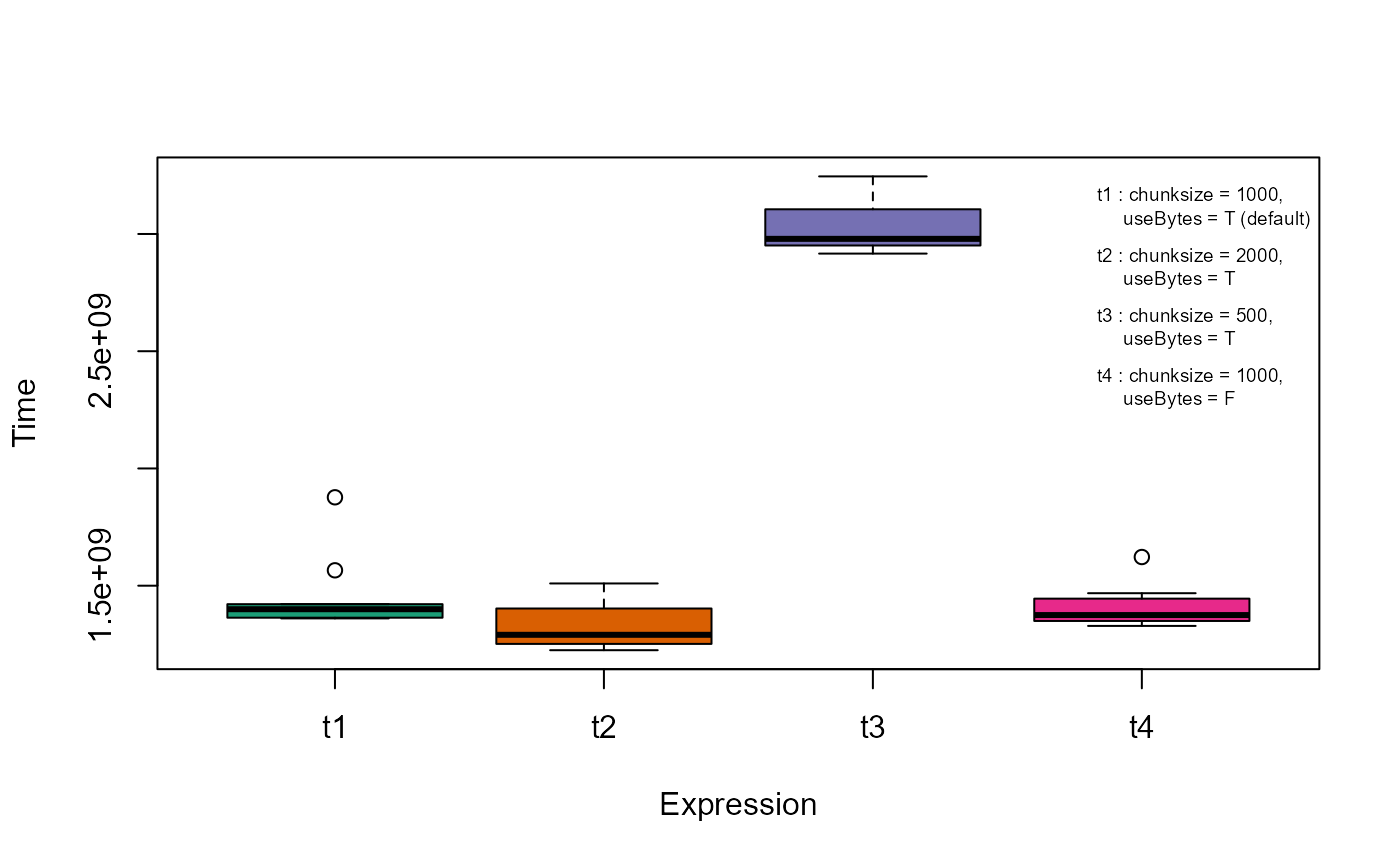
\includegraphics{Introduction_files/figure-latex/unnamed-chunk-45-1.pdf}

\textbf{Fig. 3.} CPU time with different \texttt{ProbDup} arguments
estimated using the \texttt{microbenchmark} package.

\hypertarget{set-review-modification-and-validation}{%
\subsection{Set Review, Modification and
Validation}\label{set-review-modification-and-validation}}

The initially retrieved sets may be intersecting with each other because
there might be accessions which occur in more than duplicate set.
Disjoint sets can be generated by merging such overlapping sets using
the function \texttt{DisProbDup}.

Disjoint sets are retrieved either individually for each type of
probable duplicate sets or considering all type of sets simultaneously.
In case of the latter, the disjoint of all the type of sets alone are
returned in the output as an additional data frame
\texttt{DisjointDupicates} in an object of class \texttt{ProbDup}.

\begin{Shaded}
\begin{Highlighting}[]
\CommentTok{# Load example dataset}
\NormalTok{GN <-}\StringTok{ }\NormalTok{GN1000}

\CommentTok{# Specify as a vector the database fields to be used}
\NormalTok{GNfields <-}\StringTok{ }\KeywordTok{c}\NormalTok{(}\StringTok{"NationalID"}\NormalTok{, }\StringTok{"CollNo"}\NormalTok{, }\StringTok{"DonorID"}\NormalTok{, }\StringTok{"OtherID1"}\NormalTok{, }\StringTok{"OtherID2"}\NormalTok{)}

\CommentTok{# Clean the data}
\NormalTok{GN[GNfields] <-}\StringTok{ }\KeywordTok{lapply}\NormalTok{(GN[GNfields], }\ControlFlowTok{function}\NormalTok{(x) }\KeywordTok{DataClean}\NormalTok{(x))}
\NormalTok{y1 <-}\StringTok{ }\KeywordTok{list}\NormalTok{(}\KeywordTok{c}\NormalTok{(}\StringTok{"Gujarat"}\NormalTok{, }\StringTok{"Dwarf"}\NormalTok{), }\KeywordTok{c}\NormalTok{(}\StringTok{"Castle"}\NormalTok{, }\StringTok{"Cary"}\NormalTok{), }\KeywordTok{c}\NormalTok{(}\StringTok{"Small"}\NormalTok{, }\StringTok{"Japan"}\NormalTok{),}
\KeywordTok{c}\NormalTok{(}\StringTok{"Big"}\NormalTok{, }\StringTok{"Japan"}\NormalTok{), }\KeywordTok{c}\NormalTok{(}\StringTok{"Mani"}\NormalTok{, }\StringTok{"Blanco"}\NormalTok{), }\KeywordTok{c}\NormalTok{(}\StringTok{"Uganda"}\NormalTok{, }\StringTok{"Erect"}\NormalTok{),}
\KeywordTok{c}\NormalTok{(}\StringTok{"Mota"}\NormalTok{, }\StringTok{"Company"}\NormalTok{))}
\NormalTok{y2 <-}\StringTok{ }\KeywordTok{c}\NormalTok{(}\StringTok{"Dark"}\NormalTok{, }\StringTok{"Light"}\NormalTok{, }\StringTok{"Small"}\NormalTok{, }\StringTok{"Improved"}\NormalTok{, }\StringTok{"Punjab"}\NormalTok{, }\StringTok{"SAM"}\NormalTok{)}
\NormalTok{y3 <-}\StringTok{ }\KeywordTok{c}\NormalTok{(}\StringTok{"Local"}\NormalTok{, }\StringTok{"Bold"}\NormalTok{, }\StringTok{"Cary"}\NormalTok{, }\StringTok{"Mutant"}\NormalTok{, }\StringTok{"Runner"}\NormalTok{, }\StringTok{"Giant"}\NormalTok{, }\StringTok{"No."}\NormalTok{,}
        \StringTok{"Bunch"}\NormalTok{, }\StringTok{"Peanut"}\NormalTok{)}
\NormalTok{GN[GNfields] <-}\StringTok{ }\KeywordTok{lapply}\NormalTok{(GN[GNfields],}
                       \ControlFlowTok{function}\NormalTok{(x) }\KeywordTok{MergeKW}\NormalTok{(x, y1, }\DataTypeTok{delim =} \KeywordTok{c}\NormalTok{(}\StringTok{"space"}\NormalTok{, }\StringTok{"dash"}\NormalTok{)))}
\NormalTok{GN[GNfields] <-}\StringTok{ }\KeywordTok{lapply}\NormalTok{(GN[GNfields],}
                       \ControlFlowTok{function}\NormalTok{(x) }\KeywordTok{MergePrefix}\NormalTok{(x, y2, }\DataTypeTok{delim =} \KeywordTok{c}\NormalTok{(}\StringTok{"space"}\NormalTok{, }\StringTok{"dash"}\NormalTok{)))}
\NormalTok{GN[GNfields] <-}\StringTok{ }\KeywordTok{lapply}\NormalTok{(GN[GNfields],}
                       \ControlFlowTok{function}\NormalTok{(x) }\KeywordTok{MergeSuffix}\NormalTok{(x, y3, }\DataTypeTok{delim =} \KeywordTok{c}\NormalTok{(}\StringTok{"space"}\NormalTok{, }\StringTok{"dash"}\NormalTok{)))}

\CommentTok{# Generate KWIC index}
\NormalTok{GNKWIC <-}\StringTok{ }\KeywordTok{KWIC}\NormalTok{(GN, GNfields)}

\CommentTok{# Specify the exceptions as a vector}
\NormalTok{exep <-}\StringTok{ }\KeywordTok{c}\NormalTok{(}\StringTok{"A"}\NormalTok{, }\StringTok{"B"}\NormalTok{, }\StringTok{"BIG"}\NormalTok{, }\StringTok{"BOLD"}\NormalTok{, }\StringTok{"BUNCH"}\NormalTok{, }\StringTok{"C"}\NormalTok{, }\StringTok{"COMPANY"}\NormalTok{, }\StringTok{"CULTURE"}\NormalTok{,}
         \StringTok{"DARK"}\NormalTok{, }\StringTok{"E"}\NormalTok{, }\StringTok{"EARLY"}\NormalTok{, }\StringTok{"EC"}\NormalTok{, }\StringTok{"ERECT"}\NormalTok{, }\StringTok{"EXOTIC"}\NormalTok{, }\StringTok{"FLESH"}\NormalTok{, }\StringTok{"GROUNDNUT"}\NormalTok{,}
         \StringTok{"GUTHUKAI"}\NormalTok{, }\StringTok{"IMPROVED"}\NormalTok{, }\StringTok{"K"}\NormalTok{, }\StringTok{"KUTHUKADAL"}\NormalTok{, }\StringTok{"KUTHUKAI"}\NormalTok{, }\StringTok{"LARGE"}\NormalTok{,}
         \StringTok{"LIGHT"}\NormalTok{, }\StringTok{"LOCAL"}\NormalTok{, }\StringTok{"OF"}\NormalTok{, }\StringTok{"OVERO"}\NormalTok{, }\StringTok{"P"}\NormalTok{, }\StringTok{"PEANUT"}\NormalTok{, }\StringTok{"PURPLE"}\NormalTok{, }\StringTok{"R"}\NormalTok{,}
         \StringTok{"RED"}\NormalTok{, }\StringTok{"RUNNER"}\NormalTok{, }\StringTok{"S1"}\NormalTok{, }\StringTok{"SAM"}\NormalTok{, }\StringTok{"SMALL"}\NormalTok{, }\StringTok{"SPANISH"}\NormalTok{, }\StringTok{"TAN"}\NormalTok{, }\StringTok{"TYPE"}\NormalTok{,}
         \StringTok{"U"}\NormalTok{, }\StringTok{"VALENCIA"}\NormalTok{, }\StringTok{"VIRGINIA"}\NormalTok{, }\StringTok{"WHITE"}\NormalTok{)}

\CommentTok{# Specify the synsets as a list}
\NormalTok{syn <-}\StringTok{ }\KeywordTok{list}\NormalTok{(}\KeywordTok{c}\NormalTok{(}\StringTok{"CHANDRA"}\NormalTok{, }\StringTok{"AH114"}\NormalTok{), }\KeywordTok{c}\NormalTok{(}\StringTok{"TG1"}\NormalTok{, }\StringTok{"VIKRAM"}\NormalTok{))}

\CommentTok{# Fetch probable duplicate sets}
\NormalTok{GNdup <-}\StringTok{ }\KeywordTok{ProbDup}\NormalTok{(}\DataTypeTok{kwic1 =}\NormalTok{ GNKWIC, }\DataTypeTok{method =} \StringTok{"a"}\NormalTok{, }\DataTypeTok{excep =}\NormalTok{ exep, }\DataTypeTok{fuzzy =} \OtherTok{TRUE}\NormalTok{,}
                 \DataTypeTok{phonetic =} \OtherTok{TRUE}\NormalTok{, }\DataTypeTok{encoding =} \StringTok{"primary"}\NormalTok{,}
                 \DataTypeTok{semantic =} \OtherTok{TRUE}\NormalTok{, }\DataTypeTok{syn =}\NormalTok{ syn)}
\end{Highlighting}
\end{Shaded}

\begin{Shaded}
\begin{Highlighting}[]
\CommentTok{# Initial number of sets}
\NormalTok{GNdup}
\end{Highlighting}
\end{Shaded}

\begin{verbatim}
Method : a

KWIC1 fields : NationalID CollNo DonorID OtherID1 OtherID2
 
                   No..of.Sets     No..of.Records
FuzzyDuplicates            378                745
PhoneticDuplicates          99                260
SemanticDuplicates           2                  5
Total                      479 1010(Distinct:762)
\end{verbatim}

\begin{Shaded}
\begin{Highlighting}[]
\CommentTok{# Get disjoint probable duplicate sets of each kind}
\NormalTok{disGNdup1 <-}\StringTok{ }\KeywordTok{DisProbDup}\NormalTok{(GNdup, }\DataTypeTok{combine =} \OtherTok{NULL}\NormalTok{)}
\CommentTok{# # Number of sets after combining intersecting sets}
\NormalTok{disGNdup1}
\end{Highlighting}
\end{Shaded}

\begin{verbatim}
Method : a

KWIC1 fields : NationalID CollNo DonorID OtherID1 OtherID2
 
                   No..of.Sets     No..of.Records
FuzzyDuplicates            181                745
PhoneticDuplicates          80                260
SemanticDuplicates           2                  5
Total                      263 1010(Distinct:762)
\end{verbatim}

\begin{Shaded}
\begin{Highlighting}[]
\CommentTok{# Get disjoint probable duplicate sets combining all the kinds of sets}
\NormalTok{disGNdup2 <-}\StringTok{ }\KeywordTok{DisProbDup}\NormalTok{(GNdup, }\DataTypeTok{combine =} \KeywordTok{c}\NormalTok{(}\StringTok{"F"}\NormalTok{, }\StringTok{"P"}\NormalTok{, }\StringTok{"S"}\NormalTok{))}
\CommentTok{# Number of sets after combining intersecting sets}
\NormalTok{disGNdup2}
\end{Highlighting}
\end{Shaded}

\begin{verbatim}
Method : a

KWIC1 fields : NationalID CollNo DonorID OtherID1 OtherID2
 
                  No..of.Sets    No..of.Records
DisjointDupicates         167               762
Total                     167 762(Distinct:762)
\end{verbatim}

Once duplicate sets are retrieved they can be validated by manual
clerical review by comparing with original PGR passport database(s)
using the \texttt{ReviewProbDup} function. This function helps to
retrieve PGR passport information associated with fuzzy, phonetic or
semantic probable duplicate sets in an object of class \texttt{ProbDup}
from the original databases(s) from which they were identified. The
original information of accessions comprising a set, which have not been
subjected to data standardization can be compared under manual clerical
review for the validation of the set. By default only the
fields(columns) which were used initially for creation of the KWIC
indexes using the KWIC function are retrieved. Additional
fields(columns) if necessary can be specified using the
\texttt{extra.db1} and \texttt{extra.db2} arguments.

When any primary ID/key records in the fuzzy, phonetic or semantic
duplicate sets are found to be missing from the original databases
specified in \texttt{db1} and \texttt{db2}, then they are ignored and
only the matching records are considered for retrieving the information
with a warning.

This may be due to data standardization of the primary ID/key field
using the function \texttt{DataClean} before creation of the KWIC index
and subsequent identification of probable duplicate sets. In such a
case, it is recommended to use an identical data standardization
operation on the primary ID/key field of databases specified in
\texttt{db1} and \texttt{db2} before running this function.

With \texttt{R} \textless= v3.0.2, due to copying of named objects by
\texttt{list()},
\texttt{Invalid\ .internal.selfref\ detected\ and\ fixed...} warning can
appear, which may be safely ignored.

The output data frame can be subjected to clerical review either after
exporting into an external spreadsheet using \texttt{write.csv} function
or by using the \texttt{edit} function.

The column \texttt{DEL} can be used to indicate whether a record has to
be deleted from a set or not. \texttt{Y} indicates ``Yes'', and the
default \texttt{N} indicates ``No''.

The column \texttt{SPLIT} similarly can be used to indicate whether a
record in a set has to be branched into a new set. A set of identical
integers in this column other than the default \texttt{0} can be used to
indicate that they are to be removed and assembled into a new set.

\begin{Shaded}
\begin{Highlighting}[]
\CommentTok{# Load the original database and clean the Primary ID/key field}
\NormalTok{GN1000 <-}\StringTok{ }\NormalTok{GN1000}
\NormalTok{GN1000}\OperatorTok{$}\NormalTok{NationalID <-}\StringTok{ }\KeywordTok{DataClean}\NormalTok{(GN1000}\OperatorTok{$}\NormalTok{NationalID)}

\CommentTok{# Get the data frame for reviewing the duplicate sets identified}
\NormalTok{RevGNdup <-}\StringTok{ }\KeywordTok{ReviewProbDup}\NormalTok{(}\DataTypeTok{pdup =}\NormalTok{ disGNdup1, }\DataTypeTok{db1 =}\NormalTok{ GN1000,}
                          \DataTypeTok{extra.db1 =} \KeywordTok{c}\NormalTok{(}\StringTok{"SourceCountry"}\NormalTok{, }\StringTok{"TransferYear"}\NormalTok{),}
                          \DataTypeTok{max.count =} \DecValTok{30}\NormalTok{, }\DataTypeTok{insert.blanks =} \OtherTok{TRUE}\NormalTok{)}
\end{Highlighting}
\end{Shaded}

\begin{Shaded}
\begin{Highlighting}[]
\KeywordTok{head}\NormalTok{(RevGNdup)}
\end{Highlighting}
\end{Shaded}

\begin{verbatim}
  SET_NO TYPE K[a]  PRIM_ID                IDKW  DEL SPLIT COUNT K1_NationalID                K1_CollNo K1_DonorID
1      1    F [K1] EC100277 [K1]EC100277:U44712    N     0     3      EC100277    Shulamith/ NRCG-14555   ICG-4709
2      1    F [K1]  EC21118  [K1]EC21118:U44712    N     0     3       EC21118 U 4-47-12; EC 21118; UKA    ICG3265
3      1    F [K1] IC494796 [K1]IC494796:U44712    N     0     3      IC494796                U-4-47-12   ICG-6890
4     NA      <NA>     <NA>                <NA> <NA>    NA    NA          <NA>                     <NA>       <NA>
5      1    P [K1] EC100713  [K1]EC100713:STARR    N     0    14      EC100713               EC 100713;    ICG5296
6      1    P [K1] EC106985  [K1]EC106985:STARR    N     0    14      EC106985                    Starr    ICG3479
  K1_OtherID1  K1_OtherID2        K1X_SourceCountry K1X_TransferYear
1                 U4-47-12                   Israel             2014
2             U44712 U K A                Australia             1989
3                   U44712                  Unknown             2010
4        <NA>         <NA>                     <NA>               NA
5                    STARR United States of America             2004
6                          United States of America             2001
\end{verbatim}

\begin{Shaded}
\begin{Highlighting}[]
\CommentTok{# Examine and review the duplicate sets using edit function}
\NormalTok{RevGNdup <-}\StringTok{ }\KeywordTok{edit}\NormalTok{(RevGNdup)}

\CommentTok{# OR examine and review the duplicate sets after exporting them as a csv file}
\KeywordTok{write.csv}\NormalTok{(}\DataTypeTok{file=}\StringTok{"Duplicate sets for review.csv"}\NormalTok{, }\DataTypeTok{x=}\NormalTok{RevGNdup)}
\end{Highlighting}
\end{Shaded}

After clerical review, the data frame created using the function
\texttt{ReviewProbDup} from an object of class \texttt{ProbDup} can be
reconstituted back to the same object after the review using the
function \texttt{ReconstructProbDup}.

The instructions for modifying the sets entered in the appropriate
format in the columns \texttt{DEL} and \texttt{SPLIT} during clerical
review are taken into account for reconstituting the probable duplicate
sets. Any records with \texttt{Y} in column \texttt{DEL} are deleted and
records with identical integers in the column \texttt{SPLIT} other than
the default \texttt{0} are reassembled into a new set.

\begin{Shaded}
\begin{Highlighting}[]
\CommentTok{# The original set data}
\KeywordTok{subset}\NormalTok{(RevGNdup, SET_NO}\OperatorTok{==}\DecValTok{13} \OperatorTok{&}\StringTok{ }\NormalTok{TYPE}\OperatorTok{==}\StringTok{"P"}\NormalTok{, }\DataTypeTok{select=} \KeywordTok{c}\NormalTok{(IDKW, DEL, SPLIT))}
\end{Highlighting}
\end{Shaded}

\begin{verbatim}
                                             IDKW DEL SPLIT
111                         [K1]EC38607:MANFREDI1   N     0
112                         [K1]EC420966:MANFREDI   N     0
113                        [K1]EC42549:MANFREDI68   N     0
114                          [K1]EC42550:MANFRED1   N     0
115 [K1]EC552714:CHAMPAQUI, [K1]EC552714:MANFREDI   N     0
116                       [K1]EC573128:MANFREDI84   N     0
117 [K1]IC304523:CHAMPAGUE, [K1]IC304523:MANFREDI   N     0
\end{verbatim}

\begin{Shaded}
\begin{Highlighting}[]
\CommentTok{# Make dummy changes to the set for illustration}
\NormalTok{RevGNdup[}\KeywordTok{c}\NormalTok{(}\DecValTok{113}\NormalTok{, }\DecValTok{116}\NormalTok{), }\DecValTok{6}\NormalTok{] <-}\StringTok{ "Y"}
\NormalTok{RevGNdup[}\KeywordTok{c}\NormalTok{(}\DecValTok{111}\NormalTok{, }\DecValTok{114}\NormalTok{), }\DecValTok{7}\NormalTok{] <-}\StringTok{ }\DecValTok{1}
\NormalTok{RevGNdup[}\KeywordTok{c}\NormalTok{(}\DecValTok{112}\NormalTok{, }\DecValTok{115}\NormalTok{, }\DecValTok{117}\NormalTok{), }\DecValTok{7}\NormalTok{] <-}\StringTok{ }\DecValTok{2}
\CommentTok{# The instruction for modification in columns DEL and SPLIT}
\KeywordTok{subset}\NormalTok{(RevGNdup, SET_NO}\OperatorTok{==}\DecValTok{13} \OperatorTok{&}\StringTok{ }\NormalTok{TYPE}\OperatorTok{==}\StringTok{"P"}\NormalTok{, }\DataTypeTok{select=} \KeywordTok{c}\NormalTok{(IDKW, DEL, SPLIT))}
\end{Highlighting}
\end{Shaded}

\begin{verbatim}
                                             IDKW DEL SPLIT
111                         [K1]EC38607:MANFREDI1   N     1
112                         [K1]EC420966:MANFREDI   N     2
113                        [K1]EC42549:MANFREDI68   Y     0
114                          [K1]EC42550:MANFRED1   N     1
115 [K1]EC552714:CHAMPAQUI, [K1]EC552714:MANFREDI   N     2
116                       [K1]EC573128:MANFREDI84   Y     0
117 [K1]IC304523:CHAMPAGUE, [K1]IC304523:MANFREDI   N     2
\end{verbatim}

\begin{Shaded}
\begin{Highlighting}[]
\CommentTok{# Reconstruct ProDup object}
\NormalTok{GNdup2 <-}\StringTok{ }\KeywordTok{ReconstructProbDup}\NormalTok{(RevGNdup)}
\CommentTok{# Initial no. of sets}
\NormalTok{disGNdup1}
\end{Highlighting}
\end{Shaded}

\begin{verbatim}
Method : a

KWIC1 fields : NationalID CollNo DonorID OtherID1 OtherID2
 
                   No..of.Sets     No..of.Records
FuzzyDuplicates            181                745
PhoneticDuplicates          80                260
SemanticDuplicates           2                  5
Total                      263 1010(Distinct:762)
\end{verbatim}

\begin{Shaded}
\begin{Highlighting}[]
\CommentTok{# No. of sets after modifications}
\NormalTok{GNdup2}
\end{Highlighting}
\end{Shaded}

\begin{verbatim}
Method : a

KWIC1 fields : NationalID CollNo DonorID OtherID1 OtherID2
 
                   No..of.Sets    No..of.Records
FuzzyDuplicates            180               523
PhoneticDuplicates          81               258
SemanticDuplicates           2                 5
Total                      263 786(Distinct:674)
\end{verbatim}

\hypertarget{other-functions}{%
\subsection{Other Functions}\label{other-functions}}

The \texttt{ProbDup} object is a list of data frames of different kinds
of probable duplicate sets \emph{viz}- \texttt{FuzzyDuplicates},
\texttt{PhoneticDuplicates}, \texttt{SemanticDuplicates} and
\texttt{DisjointDuplicates}. Each row of the component data frame will
have information of a set, the type of set, the set members as well as
the keywords based on which the set was formed. This data can be
reshaped into long form using the function \texttt{ParseProbDup}. This
function which will transform a \texttt{ProbDup} object into a single
data frame.

\begin{Shaded}
\begin{Highlighting}[]
\CommentTok{# Convert 'ProbDup' object to a long form data frame of sets}
\NormalTok{GNdupParsed <-}\StringTok{ }\KeywordTok{ParseProbDup}\NormalTok{(GNdup)}
\KeywordTok{head}\NormalTok{(GNdupParsed)}
\end{Highlighting}
\end{Shaded}

\begin{verbatim}
  SET_NO TYPE    K  PRIM_ID                IDKW COUNT
1      1    F [K1] EC100277 [K1]EC100277:U44712     3
2      1    F [K1]  EC21118  [K1]EC21118:U44712     3
3      1    F [K1] IC494796 [K1]IC494796:U44712     3
4     NA      <NA>     <NA>                <NA>    NA
5      2    F [K1] EC100280    [K1]EC100280:NC5     3
6      2    F [K1] EC100721    [K1]EC100721:NC5     3
\end{verbatim}

The prefix \texttt{K*} here indicates the KWIC index of origin. This is
useful in ascertaining the database of origin of the accessions when
method \texttt{"b"} or \texttt{"c"} was used to create the input
\texttt{ProbDup} object.

Once the sets are reviewed and modified, the validated set data fields
from the \texttt{ProbDup} object can be added to the original PGR
passport database using the function \texttt{AddProbDup}. The associated
data fields such as \texttt{SET\_NO}, \texttt{ID} and \texttt{IDKW} are
added based on the \texttt{PRIM\_ID} field(column).

\begin{Shaded}
\begin{Highlighting}[]
\CommentTok{# Loading original database}
\NormalTok{GN2 <-}\StringTok{ }\NormalTok{GN1000}

\CommentTok{# Add the duplicates set data to the original database}
\NormalTok{GNwithdup <-}\StringTok{  }\KeywordTok{AddProbDup}\NormalTok{(}\DataTypeTok{pdup =}\NormalTok{ GNdup, }\DataTypeTok{db =}\NormalTok{ GN2, }\DataTypeTok{addto =} \StringTok{"I"}\NormalTok{)}
\end{Highlighting}
\end{Shaded}

In case more than one KWIC index was used to generate the object of
class \texttt{ProbDup}, the argument \texttt{addto} can be used to
specify to which database the data fields are to be added. The default
\texttt{"I"} indicates the database from which the first KWIC index was
created and \texttt{"II"} indicates the database from which the second
index was created.

The function \texttt{SplitProbDup} can be used to split an object of
class \texttt{ProbDup} into two on the basis of set counts. This is
useful for reviewing separately the sets with larger set counts.

\begin{Shaded}
\begin{Highlighting}[]
\CommentTok{# Load PGR passport database}
\NormalTok{GN <-}\StringTok{ }\NormalTok{GN1000}

\CommentTok{# Specify as a vector the database fields to be used}
\NormalTok{GNfields <-}\StringTok{ }\KeywordTok{c}\NormalTok{(}\StringTok{"NationalID"}\NormalTok{, }\StringTok{"CollNo"}\NormalTok{, }\StringTok{"DonorID"}\NormalTok{, }\StringTok{"OtherID1"}\NormalTok{, }\StringTok{"OtherID2"}\NormalTok{)}

\CommentTok{# Clean the data}
\NormalTok{GN[GNfields] <-}\StringTok{ }\KeywordTok{lapply}\NormalTok{(GN[GNfields], }\ControlFlowTok{function}\NormalTok{(x) }\KeywordTok{DataClean}\NormalTok{(x))}
\NormalTok{y1 <-}\StringTok{ }\KeywordTok{list}\NormalTok{(}\KeywordTok{c}\NormalTok{(}\StringTok{"Gujarat"}\NormalTok{, }\StringTok{"Dwarf"}\NormalTok{), }\KeywordTok{c}\NormalTok{(}\StringTok{"Castle"}\NormalTok{, }\StringTok{"Cary"}\NormalTok{), }\KeywordTok{c}\NormalTok{(}\StringTok{"Small"}\NormalTok{, }\StringTok{"Japan"}\NormalTok{),}
\KeywordTok{c}\NormalTok{(}\StringTok{"Big"}\NormalTok{, }\StringTok{"Japan"}\NormalTok{), }\KeywordTok{c}\NormalTok{(}\StringTok{"Mani"}\NormalTok{, }\StringTok{"Blanco"}\NormalTok{), }\KeywordTok{c}\NormalTok{(}\StringTok{"Uganda"}\NormalTok{, }\StringTok{"Erect"}\NormalTok{),}
\KeywordTok{c}\NormalTok{(}\StringTok{"Mota"}\NormalTok{, }\StringTok{"Company"}\NormalTok{))}
\NormalTok{y2 <-}\StringTok{ }\KeywordTok{c}\NormalTok{(}\StringTok{"Dark"}\NormalTok{, }\StringTok{"Light"}\NormalTok{, }\StringTok{"Small"}\NormalTok{, }\StringTok{"Improved"}\NormalTok{, }\StringTok{"Punjab"}\NormalTok{, }\StringTok{"SAM"}\NormalTok{)}
\NormalTok{y3 <-}\StringTok{ }\KeywordTok{c}\NormalTok{(}\StringTok{"Local"}\NormalTok{, }\StringTok{"Bold"}\NormalTok{, }\StringTok{"Cary"}\NormalTok{, }\StringTok{"Mutant"}\NormalTok{, }\StringTok{"Runner"}\NormalTok{, }\StringTok{"Giant"}\NormalTok{, }\StringTok{"No."}\NormalTok{,}
        \StringTok{"Bunch"}\NormalTok{, }\StringTok{"Peanut"}\NormalTok{)}
\NormalTok{GN[GNfields] <-}\StringTok{ }\KeywordTok{lapply}\NormalTok{(GN[GNfields],}
                       \ControlFlowTok{function}\NormalTok{(x) }\KeywordTok{MergeKW}\NormalTok{(x, y1, }\DataTypeTok{delim =} \KeywordTok{c}\NormalTok{(}\StringTok{"space"}\NormalTok{, }\StringTok{"dash"}\NormalTok{)))}
\NormalTok{GN[GNfields] <-}\StringTok{ }\KeywordTok{lapply}\NormalTok{(GN[GNfields],}
                       \ControlFlowTok{function}\NormalTok{(x) }\KeywordTok{MergePrefix}\NormalTok{(x, y2, }\DataTypeTok{delim =} \KeywordTok{c}\NormalTok{(}\StringTok{"space"}\NormalTok{, }\StringTok{"dash"}\NormalTok{)))}
\NormalTok{GN[GNfields] <-}\StringTok{ }\KeywordTok{lapply}\NormalTok{(GN[GNfields],}
                       \ControlFlowTok{function}\NormalTok{(x) }\KeywordTok{MergeSuffix}\NormalTok{(x, y3, }\DataTypeTok{delim =} \KeywordTok{c}\NormalTok{(}\StringTok{"space"}\NormalTok{, }\StringTok{"dash"}\NormalTok{)))}

\CommentTok{# Generate KWIC index}
\NormalTok{GNKWIC <-}\StringTok{ }\KeywordTok{KWIC}\NormalTok{(GN, GNfields)}

\CommentTok{# Specify the exceptions as a vector}
\NormalTok{exep <-}\StringTok{ }\KeywordTok{c}\NormalTok{(}\StringTok{"A"}\NormalTok{, }\StringTok{"B"}\NormalTok{, }\StringTok{"BIG"}\NormalTok{, }\StringTok{"BOLD"}\NormalTok{, }\StringTok{"BUNCH"}\NormalTok{, }\StringTok{"C"}\NormalTok{, }\StringTok{"COMPANY"}\NormalTok{, }\StringTok{"CULTURE"}\NormalTok{,}
         \StringTok{"DARK"}\NormalTok{, }\StringTok{"E"}\NormalTok{, }\StringTok{"EARLY"}\NormalTok{, }\StringTok{"EC"}\NormalTok{, }\StringTok{"ERECT"}\NormalTok{, }\StringTok{"EXOTIC"}\NormalTok{, }\StringTok{"FLESH"}\NormalTok{, }\StringTok{"GROUNDNUT"}\NormalTok{,}
         \StringTok{"GUTHUKAI"}\NormalTok{, }\StringTok{"IMPROVED"}\NormalTok{, }\StringTok{"K"}\NormalTok{, }\StringTok{"KUTHUKADAL"}\NormalTok{, }\StringTok{"KUTHUKAI"}\NormalTok{, }\StringTok{"LARGE"}\NormalTok{,}
         \StringTok{"LIGHT"}\NormalTok{, }\StringTok{"LOCAL"}\NormalTok{, }\StringTok{"OF"}\NormalTok{, }\StringTok{"OVERO"}\NormalTok{, }\StringTok{"P"}\NormalTok{, }\StringTok{"PEANUT"}\NormalTok{, }\StringTok{"PURPLE"}\NormalTok{, }\StringTok{"R"}\NormalTok{,}
         \StringTok{"RED"}\NormalTok{, }\StringTok{"RUNNER"}\NormalTok{, }\StringTok{"S1"}\NormalTok{, }\StringTok{"SAM"}\NormalTok{, }\StringTok{"SMALL"}\NormalTok{, }\StringTok{"SPANISH"}\NormalTok{, }\StringTok{"TAN"}\NormalTok{, }\StringTok{"TYPE"}\NormalTok{,}
         \StringTok{"U"}\NormalTok{, }\StringTok{"VALENCIA"}\NormalTok{, }\StringTok{"VIRGINIA"}\NormalTok{, }\StringTok{"WHITE"}\NormalTok{)}

\CommentTok{# Specify the synsets as a list}
\NormalTok{syn <-}\StringTok{ }\KeywordTok{list}\NormalTok{(}\KeywordTok{c}\NormalTok{(}\StringTok{"CHANDRA"}\NormalTok{, }\StringTok{"AH114"}\NormalTok{), }\KeywordTok{c}\NormalTok{(}\StringTok{"TG1"}\NormalTok{, }\StringTok{"VIKRAM"}\NormalTok{))}

\CommentTok{# Fetch probable duplicate sets}
\NormalTok{GNdup <-}\StringTok{ }\KeywordTok{ProbDup}\NormalTok{(}\DataTypeTok{kwic1 =}\NormalTok{ GNKWIC, }\DataTypeTok{method =} \StringTok{"a"}\NormalTok{, }\DataTypeTok{excep =}\NormalTok{ exep, }\DataTypeTok{fuzzy =} \OtherTok{TRUE}\NormalTok{,}
                 \DataTypeTok{phonetic =} \OtherTok{TRUE}\NormalTok{, }\DataTypeTok{encoding =} \StringTok{"primary"}\NormalTok{,}
                 \DataTypeTok{semantic =} \OtherTok{TRUE}\NormalTok{, }\DataTypeTok{syn =}\NormalTok{ syn)}
\end{Highlighting}
\end{Shaded}

\begin{Shaded}
\begin{Highlighting}[]
\CommentTok{# Split the probable duplicate sets}
\NormalTok{GNdupSplit <-}\StringTok{ }\KeywordTok{SplitProbDup}\NormalTok{(GNdup, }\DataTypeTok{splitat =} \KeywordTok{c}\NormalTok{(}\DecValTok{10}\NormalTok{, }\DecValTok{10}\NormalTok{, }\DecValTok{10}\NormalTok{))}
\NormalTok{GNdupSplit[[}\DecValTok{1}\NormalTok{]]}
\end{Highlighting}
\end{Shaded}

\begin{verbatim}
Method : a

KWIC1 fields : NationalID CollNo DonorID OtherID1 OtherID2
 
                   No..of.Sets     No..of.Records
FuzzyDuplicates            338                744
PhoneticDuplicates          99                260
SemanticDuplicates           2                  5
Total                      439 1009(Distinct:762)
\end{verbatim}

\begin{Shaded}
\begin{Highlighting}[]
\NormalTok{GNdupSplit[[}\DecValTok{3}\NormalTok{]]}
\end{Highlighting}
\end{Shaded}

\begin{verbatim}
Method : a

KWIC1 fields : NationalID CollNo DonorID OtherID1 OtherID2
 
                No..of.Sets    No..of.Records
FuzzyDuplicates          40               136
Total                    40 136(Distinct:136)
\end{verbatim}

Alternatively, two different \texttt{ProbDup} objects can be merged
together using the function \texttt{MergeProbDup}.

\begin{Shaded}
\begin{Highlighting}[]
\NormalTok{GNdupMerged <-}\StringTok{ }\KeywordTok{MergeProbDup}\NormalTok{(GNdupSplit[[}\DecValTok{1}\NormalTok{]], GNdupSplit[[}\DecValTok{3}\NormalTok{]])}
\NormalTok{GNdupMerged}
\end{Highlighting}
\end{Shaded}

\begin{verbatim}
Method : a

KWIC1 fields : NationalID CollNo DonorID OtherID1 OtherID2
 
                   No..of.Sets     No..of.Records
FuzzyDuplicates            378                745
PhoneticDuplicates          99                260
SemanticDuplicates           2                  5
Total                      479 1010(Distinct:762)
\end{verbatim}

The summary of accessions according to a grouping factor field(column)
in the original database(s) within the probable duplicate sets retrieved
in a \texttt{ProbDup} object can be visualized by the
\texttt{ViewProbDup} function. The resulting plot can be used to examine
the extent of probable duplication within and between groups of
accessions records.

\begin{Shaded}
\begin{Highlighting}[]
\CommentTok{# Load PGR passport databases}
\NormalTok{GN1 <-}\StringTok{ }\NormalTok{GN1000[}\OperatorTok{!}\KeywordTok{grepl}\NormalTok{(}\StringTok{"^ICG"}\NormalTok{, GN1000}\OperatorTok{$}\NormalTok{DonorID), ]}
\NormalTok{GN1}\OperatorTok{$}\NormalTok{DonorID <-}\StringTok{ }\OtherTok{NULL}
\NormalTok{GN2 <-}\StringTok{ }\NormalTok{GN1000[}\KeywordTok{grepl}\NormalTok{(}\StringTok{"^ICG"}\NormalTok{, GN1000}\OperatorTok{$}\NormalTok{DonorID), ]}
\NormalTok{GN2 <-}\StringTok{ }\NormalTok{GN2[}\OperatorTok{!}\KeywordTok{grepl}\NormalTok{(}\StringTok{"S"}\NormalTok{, GN2}\OperatorTok{$}\NormalTok{DonorID), ]}
\NormalTok{GN2}\OperatorTok{$}\NormalTok{NationalID <-}\StringTok{ }\OtherTok{NULL}

\NormalTok{GN1}\OperatorTok{$}\NormalTok{SourceCountry <-}\StringTok{ }\KeywordTok{toupper}\NormalTok{(GN1}\OperatorTok{$}\NormalTok{SourceCountry)}
\NormalTok{GN2}\OperatorTok{$}\NormalTok{SourceCountry <-}\StringTok{ }\KeywordTok{toupper}\NormalTok{(GN2}\OperatorTok{$}\NormalTok{SourceCountry)}

\NormalTok{GN1}\OperatorTok{$}\NormalTok{SourceCountry <-}\StringTok{ }\KeywordTok{gsub}\NormalTok{(}\StringTok{"UNITED STATES OF AMERICA"}\NormalTok{, }\StringTok{"USA"}\NormalTok{, GN1}\OperatorTok{$}\NormalTok{SourceCountry)}
\NormalTok{GN2}\OperatorTok{$}\NormalTok{SourceCountry <-}\StringTok{ }\KeywordTok{gsub}\NormalTok{(}\StringTok{"UNITED STATES OF AMERICA"}\NormalTok{, }\StringTok{"USA"}\NormalTok{, GN2}\OperatorTok{$}\NormalTok{SourceCountry)}

\CommentTok{# Specify as a vector the database fields to be used}
\NormalTok{GN1fields <-}\StringTok{ }\KeywordTok{c}\NormalTok{(}\StringTok{"NationalID"}\NormalTok{, }\StringTok{"CollNo"}\NormalTok{, }\StringTok{"OtherID1"}\NormalTok{, }\StringTok{"OtherID2"}\NormalTok{)}
\NormalTok{GN2fields <-}\StringTok{ }\KeywordTok{c}\NormalTok{(}\StringTok{"DonorID"}\NormalTok{, }\StringTok{"CollNo"}\NormalTok{, }\StringTok{"OtherID1"}\NormalTok{, }\StringTok{"OtherID2"}\NormalTok{)}

\CommentTok{# Clean the data}
\NormalTok{GN1[GN1fields] <-}\StringTok{ }\KeywordTok{lapply}\NormalTok{(GN1[GN1fields], }\ControlFlowTok{function}\NormalTok{(x) }\KeywordTok{DataClean}\NormalTok{(x))}
\NormalTok{GN2[GN2fields] <-}\StringTok{ }\KeywordTok{lapply}\NormalTok{(GN2[GN2fields], }\ControlFlowTok{function}\NormalTok{(x) }\KeywordTok{DataClean}\NormalTok{(x))}
\NormalTok{y1 <-}\StringTok{ }\KeywordTok{list}\NormalTok{(}\KeywordTok{c}\NormalTok{(}\StringTok{"Gujarat"}\NormalTok{, }\StringTok{"Dwarf"}\NormalTok{), }\KeywordTok{c}\NormalTok{(}\StringTok{"Castle"}\NormalTok{, }\StringTok{"Cary"}\NormalTok{), }\KeywordTok{c}\NormalTok{(}\StringTok{"Small"}\NormalTok{, }\StringTok{"Japan"}\NormalTok{),}
           \KeywordTok{c}\NormalTok{(}\StringTok{"Big"}\NormalTok{, }\StringTok{"Japan"}\NormalTok{), }\KeywordTok{c}\NormalTok{(}\StringTok{"Mani"}\NormalTok{, }\StringTok{"Blanco"}\NormalTok{), }\KeywordTok{c}\NormalTok{(}\StringTok{"Uganda"}\NormalTok{, }\StringTok{"Erect"}\NormalTok{),}
           \KeywordTok{c}\NormalTok{(}\StringTok{"Mota"}\NormalTok{, }\StringTok{"Company"}\NormalTok{))}
\NormalTok{y2 <-}\StringTok{ }\KeywordTok{c}\NormalTok{(}\StringTok{"Dark"}\NormalTok{, }\StringTok{"Light"}\NormalTok{, }\StringTok{"Small"}\NormalTok{, }\StringTok{"Improved"}\NormalTok{, }\StringTok{"Punjab"}\NormalTok{, }\StringTok{"SAM"}\NormalTok{)}
\NormalTok{y3 <-}\StringTok{ }\KeywordTok{c}\NormalTok{(}\StringTok{"Local"}\NormalTok{, }\StringTok{"Bold"}\NormalTok{, }\StringTok{"Cary"}\NormalTok{, }\StringTok{"Mutant"}\NormalTok{, }\StringTok{"Runner"}\NormalTok{, }\StringTok{"Giant"}\NormalTok{, }\StringTok{"No."}\NormalTok{,}
        \StringTok{"Bunch"}\NormalTok{, }\StringTok{"Peanut"}\NormalTok{)}
\NormalTok{GN1[GN1fields] <-}\StringTok{ }\KeywordTok{lapply}\NormalTok{(GN1[GN1fields],}
                         \ControlFlowTok{function}\NormalTok{(x) }\KeywordTok{MergeKW}\NormalTok{(x, y1, }\DataTypeTok{delim =} \KeywordTok{c}\NormalTok{(}\StringTok{"space"}\NormalTok{, }\StringTok{"dash"}\NormalTok{)))}
\NormalTok{GN1[GN1fields] <-}\StringTok{ }\KeywordTok{lapply}\NormalTok{(GN1[GN1fields],}
                         \ControlFlowTok{function}\NormalTok{(x) }\KeywordTok{MergePrefix}\NormalTok{(x, y2, }\DataTypeTok{delim =} \KeywordTok{c}\NormalTok{(}\StringTok{"space"}\NormalTok{, }\StringTok{"dash"}\NormalTok{)))}
\NormalTok{GN1[GN1fields] <-}\StringTok{ }\KeywordTok{lapply}\NormalTok{(GN1[GN1fields],}
                         \ControlFlowTok{function}\NormalTok{(x) }\KeywordTok{MergeSuffix}\NormalTok{(x, y3, }\DataTypeTok{delim =} \KeywordTok{c}\NormalTok{(}\StringTok{"space"}\NormalTok{, }\StringTok{"dash"}\NormalTok{)))}
\NormalTok{GN2[GN2fields] <-}\StringTok{ }\KeywordTok{lapply}\NormalTok{(GN2[GN2fields],}
                         \ControlFlowTok{function}\NormalTok{(x) }\KeywordTok{MergeKW}\NormalTok{(x, y1, }\DataTypeTok{delim =} \KeywordTok{c}\NormalTok{(}\StringTok{"space"}\NormalTok{, }\StringTok{"dash"}\NormalTok{)))}
\NormalTok{GN2[GN2fields] <-}\StringTok{ }\KeywordTok{lapply}\NormalTok{(GN2[GN2fields],}
                         \ControlFlowTok{function}\NormalTok{(x) }\KeywordTok{MergePrefix}\NormalTok{(x, y2, }\DataTypeTok{delim =} \KeywordTok{c}\NormalTok{(}\StringTok{"space"}\NormalTok{, }\StringTok{"dash"}\NormalTok{)))}
\NormalTok{GN2[GN2fields] <-}\StringTok{ }\KeywordTok{lapply}\NormalTok{(GN2[GN2fields],}
                         \ControlFlowTok{function}\NormalTok{(x) }\KeywordTok{MergeSuffix}\NormalTok{(x, y3, }\DataTypeTok{delim =} \KeywordTok{c}\NormalTok{(}\StringTok{"space"}\NormalTok{, }\StringTok{"dash"}\NormalTok{)))}

\CommentTok{# Remove duplicated DonorID records in GN2}
\NormalTok{GN2 <-}\StringTok{ }\NormalTok{GN2[}\OperatorTok{!}\KeywordTok{duplicated}\NormalTok{(GN2}\OperatorTok{$}\NormalTok{DonorID), ]}

\CommentTok{# Generate KWIC index}
\NormalTok{GN1KWIC <-}\StringTok{ }\KeywordTok{KWIC}\NormalTok{(GN1, GN1fields)}
\NormalTok{GN2KWIC <-}\StringTok{ }\KeywordTok{KWIC}\NormalTok{(GN2, GN2fields)}

\CommentTok{# Specify the exceptions as a vector}
\NormalTok{exep <-}\StringTok{ }\KeywordTok{c}\NormalTok{(}\StringTok{"A"}\NormalTok{, }\StringTok{"B"}\NormalTok{, }\StringTok{"BIG"}\NormalTok{, }\StringTok{"BOLD"}\NormalTok{, }\StringTok{"BUNCH"}\NormalTok{, }\StringTok{"C"}\NormalTok{, }\StringTok{"COMPANY"}\NormalTok{, }\StringTok{"CULTURE"}\NormalTok{,}
          \StringTok{"DARK"}\NormalTok{, }\StringTok{"E"}\NormalTok{, }\StringTok{"EARLY"}\NormalTok{, }\StringTok{"EC"}\NormalTok{, }\StringTok{"ERECT"}\NormalTok{, }\StringTok{"EXOTIC"}\NormalTok{, }\StringTok{"FLESH"}\NormalTok{, }\StringTok{"GROUNDNUT"}\NormalTok{,}
          \StringTok{"GUTHUKAI"}\NormalTok{, }\StringTok{"IMPROVED"}\NormalTok{, }\StringTok{"K"}\NormalTok{, }\StringTok{"KUTHUKADAL"}\NormalTok{, }\StringTok{"KUTHUKAI"}\NormalTok{, }\StringTok{"LARGE"}\NormalTok{,}
          \StringTok{"LIGHT"}\NormalTok{, }\StringTok{"LOCAL"}\NormalTok{, }\StringTok{"OF"}\NormalTok{, }\StringTok{"OVERO"}\NormalTok{, }\StringTok{"P"}\NormalTok{, }\StringTok{"PEANUT"}\NormalTok{, }\StringTok{"PURPLE"}\NormalTok{, }\StringTok{"R"}\NormalTok{,}
          \StringTok{"RED"}\NormalTok{, }\StringTok{"RUNNER"}\NormalTok{, }\StringTok{"S1"}\NormalTok{, }\StringTok{"SAM"}\NormalTok{, }\StringTok{"SMALL"}\NormalTok{, }\StringTok{"SPANISH"}\NormalTok{, }\StringTok{"TAN"}\NormalTok{, }\StringTok{"TYPE"}\NormalTok{,}
          \StringTok{"U"}\NormalTok{, }\StringTok{"VALENCIA"}\NormalTok{, }\StringTok{"VIRGINIA"}\NormalTok{, }\StringTok{"WHITE"}\NormalTok{)}

\CommentTok{# Specify the synsets as a list}
\NormalTok{syn <-}\StringTok{ }\KeywordTok{list}\NormalTok{(}\KeywordTok{c}\NormalTok{(}\StringTok{"CHANDRA"}\NormalTok{, }\StringTok{"AH114"}\NormalTok{), }\KeywordTok{c}\NormalTok{(}\StringTok{"TG1"}\NormalTok{, }\StringTok{"VIKRAM"}\NormalTok{))}
\end{Highlighting}
\end{Shaded}

\begin{Shaded}
\begin{Highlighting}[]
\NormalTok{GNdupc <-}\StringTok{ }\KeywordTok{ProbDup}\NormalTok{(}\DataTypeTok{kwic1 =}\NormalTok{ GN1KWIC, }\DataTypeTok{kwic2 =}\NormalTok{ GN2KWIC, }\DataTypeTok{method =} \StringTok{"c"}\NormalTok{,}
                  \DataTypeTok{excep =}\NormalTok{ exep, }\DataTypeTok{fuzzy =} \OtherTok{TRUE}\NormalTok{, }\DataTypeTok{phonetic =} \OtherTok{TRUE}\NormalTok{,}
                  \DataTypeTok{encoding =} \StringTok{"primary"}\NormalTok{, }\DataTypeTok{semantic =} \OtherTok{TRUE}\NormalTok{, }\DataTypeTok{syn =}\NormalTok{ syn)}
\end{Highlighting}
\end{Shaded}

\begin{verbatim}
Fuzzy matching
\end{verbatim}

\begin{verbatim}
  |                                                                                                                       |=====================================                                                                          |  33%Block 1 / 3 |  |                                                                                                                       |==========================================================================                                     |  67%Block 2 / 3 |  |                                                                                                                       |===============================================================================================================| 100%Block 3 / 3 |
\end{verbatim}

\begin{verbatim}
Phonetic matching
\end{verbatim}

\begin{verbatim}
  |                                                                                                                       |=====================================                                                                          |  33%Block 1 / 3 |  |                                                                                                                       |==========================================================================                                     |  67%Block 2 / 3 |  |                                                                                                                       |===============================================================================================================| 100%Block 3 / 3 |
\end{verbatim}

\begin{verbatim}
Semantic matching
\end{verbatim}

\begin{verbatim}
  |                                                                                                                       |=====================================                                                                          |  33%Block 1 / 3 |  |                                                                                                                       |==========================================================================                                     |  67%Block 2 / 3 |  |                                                                                                                       |===============================================================================================================| 100%Block 3 / 3 |
\end{verbatim}

\begin{Shaded}
\begin{Highlighting}[]
\CommentTok{# Get the summary data.frames and Grob}
\NormalTok{GNdupcView <-}\StringTok{ }\KeywordTok{ViewProbDup}\NormalTok{(GNdupc, GN1, GN2, }\StringTok{"SourceCountry"}\NormalTok{, }\StringTok{"SourceCountry"}\NormalTok{,}
                         \DataTypeTok{max.count =} \DecValTok{30}\NormalTok{, }\DataTypeTok{select =} \KeywordTok{c}\NormalTok{(}\StringTok{"INDIA"}\NormalTok{, }\StringTok{"USA"}\NormalTok{), }\DataTypeTok{order =} \StringTok{"type"}\NormalTok{,}
                         \DataTypeTok{main =} \StringTok{"Groundnut Probable Duplicates"}\NormalTok{)}
\end{Highlighting}
\end{Shaded}

\begin{Shaded}
\begin{Highlighting}[]
\CommentTok{# View the summary data.frames}
\NormalTok{GNdupcView[[}\DecValTok{1}\NormalTok{]]}
\NormalTok{GNdupcView[[}\DecValTok{2}\NormalTok{]]}
\end{Highlighting}
\end{Shaded}

\begin{Shaded}
\begin{Highlighting}[]
\CommentTok{# Plot the summary visualization}
\KeywordTok{library}\NormalTok{(gridExtra)}
\KeywordTok{grid.arrange}\NormalTok{(GNdupcView[[}\DecValTok{3}\NormalTok{]])}
\end{Highlighting}
\end{Shaded}

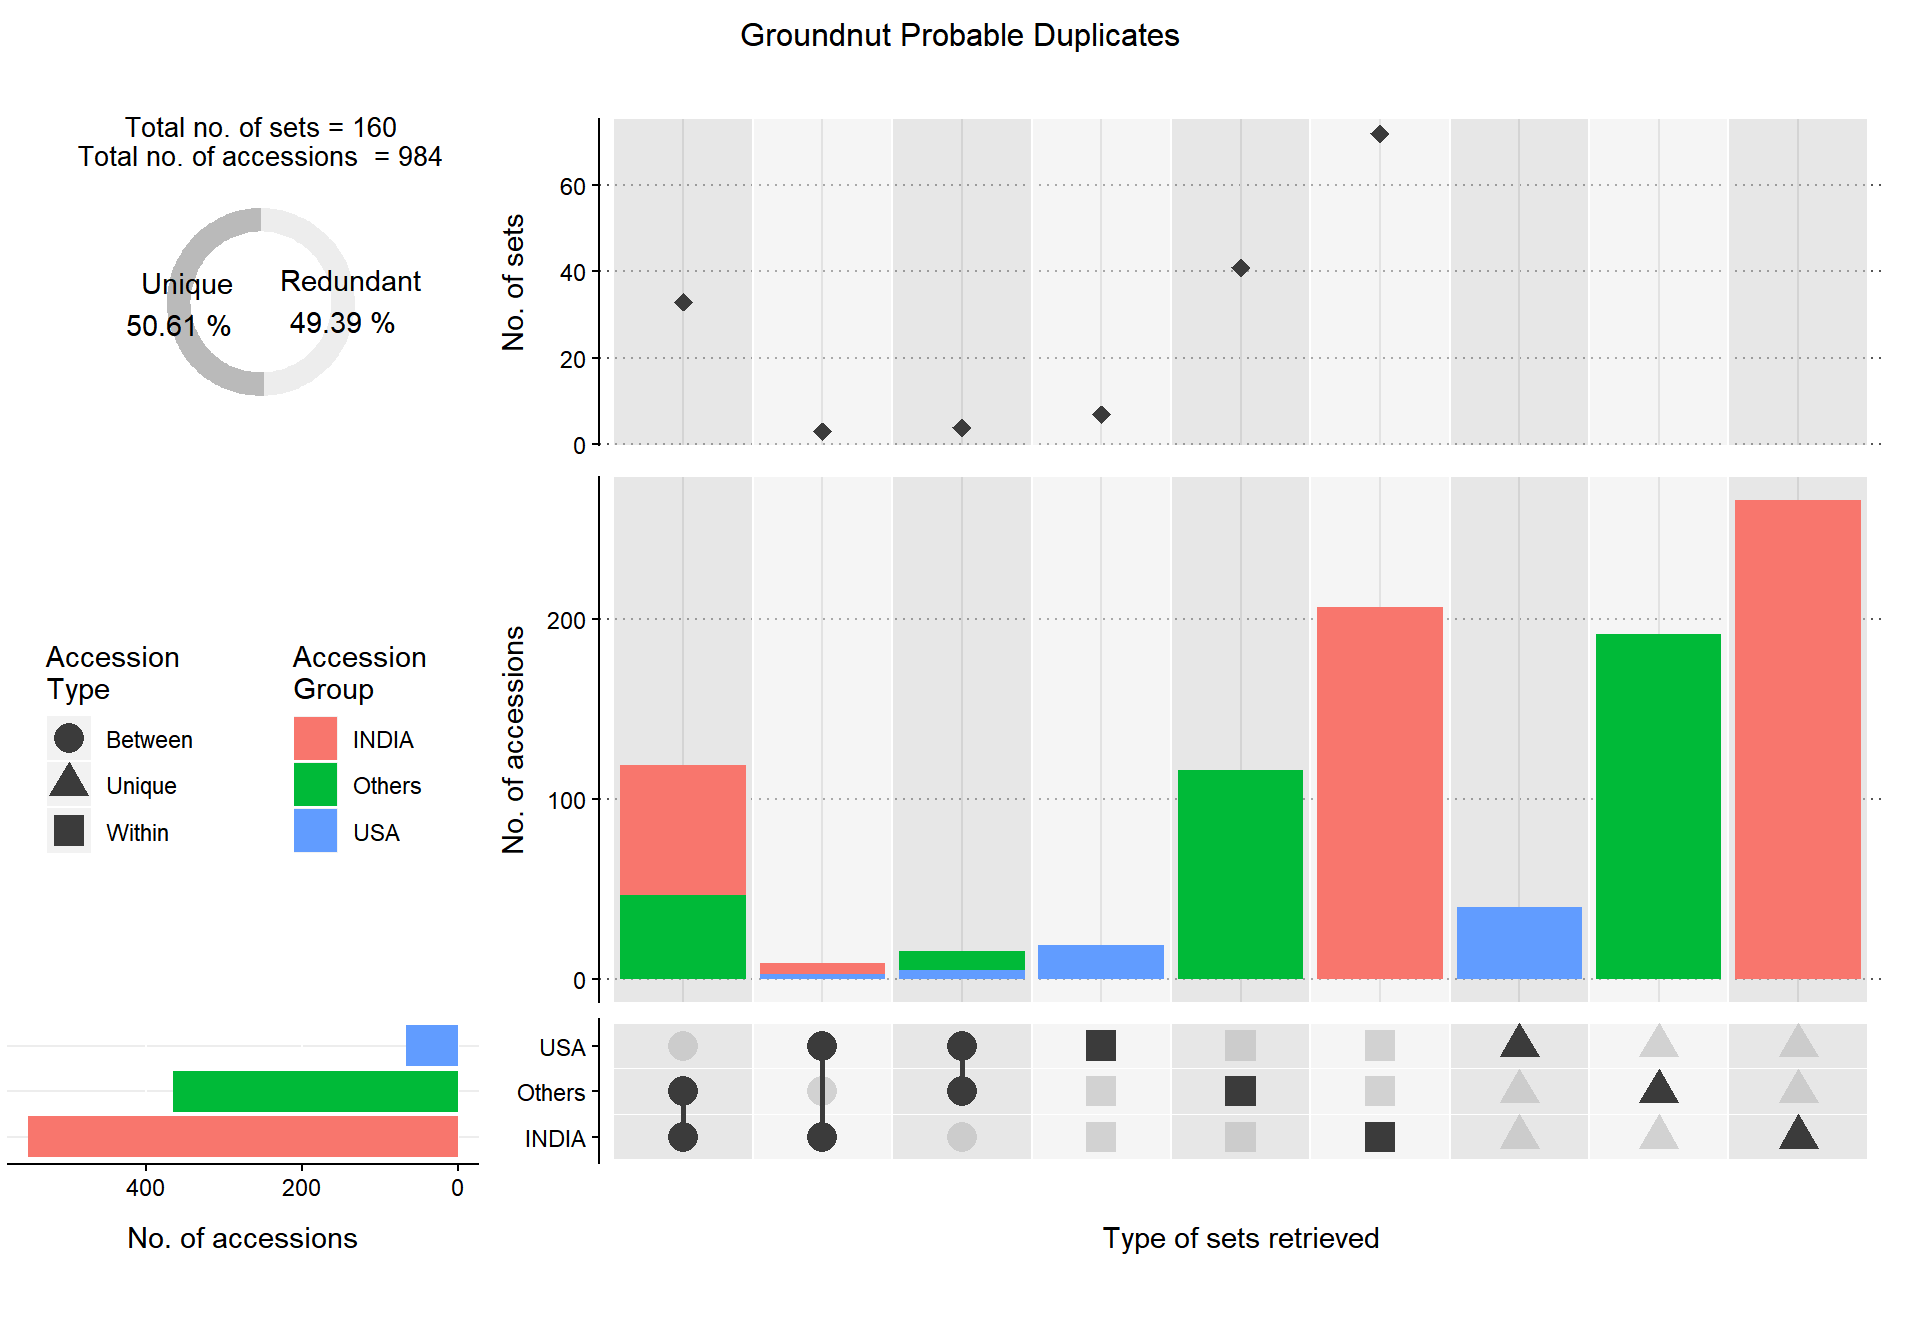
\includegraphics{Introduction_files/figure-latex/unnamed-chunk-60-1.pdf}

\textbf{Fig. 5.} Summary visualization of groundnut probable duplicate
sets retrieved according to \texttt{SourceCountry} field.

The function \texttt{KWCounts} can be used to compute the keyword counts
from PGR passport database fields(columns) which are considered for
identification of probable duplicates. These keyword counts can give a
rough indication of the completeness of the data in such fields
(Fig.~3).

\begin{Shaded}
\begin{Highlighting}[]
\CommentTok{# Compute the keyword counts for the whole data}
\NormalTok{GNKWCouts <-}\StringTok{ }\KeywordTok{KWCounts}\NormalTok{(GN, GNfields, exep)}

\CommentTok{# Compute the keyword counts for 'duplicated' records}
\NormalTok{GND <-}\StringTok{ }\KeywordTok{ParseProbDup}\NormalTok{(disGNdup2, }\OtherTok{Inf}\NormalTok{, F)}\OperatorTok{$}\NormalTok{PRIM_ID}

\NormalTok{GNDKWCouts <-}\StringTok{ }\KeywordTok{KWCounts}\NormalTok{(GN[GN}\OperatorTok{$}\NormalTok{NationalID }\OperatorTok\StringTok{ }\NormalTok{GND, ],}
\NormalTok{                       GNfields, exep)}

\CommentTok{# Compute the keyword counts for 'unique' records}
\NormalTok{GNUKWCouts <-}\StringTok{ }\KeywordTok{KWCounts}\NormalTok{(GN[}\OperatorTok{!}\NormalTok{GN}\OperatorTok{$}\NormalTok{NationalID }\OperatorTok\StringTok{ }\NormalTok{GND, ],}
\NormalTok{                       GNfields, exep)}

\CommentTok{# Plot the counts as barplot}
\KeywordTok{par}\NormalTok{(}\DataTypeTok{mfrow =} \KeywordTok{c}\NormalTok{(}\DecValTok{3}\NormalTok{,}\DecValTok{1}\NormalTok{))}

\NormalTok{bp1 <-}\StringTok{ }\KeywordTok{barplot}\NormalTok{(}\KeywordTok{table}\NormalTok{(GNKWCouts}\OperatorTok{$}\NormalTok{COUNT),}
               \DataTypeTok{xlab =} \StringTok{"Word count"}\NormalTok{, }\DataTypeTok{ylab =} \StringTok{"Frequency"}\NormalTok{,}
               \DataTypeTok{main =} \StringTok{"A"}\NormalTok{, }\DataTypeTok{col =} \StringTok{"#1B9E77"}\NormalTok{)}
\KeywordTok{text}\NormalTok{(bp1, }\DecValTok{0}\NormalTok{, }\KeywordTok{table}\NormalTok{(GNKWCouts}\OperatorTok{$}\NormalTok{COUNT),}\DataTypeTok{cex =} \DecValTok{1}\NormalTok{, }\DataTypeTok{pos =} \DecValTok{3}\NormalTok{)}
\KeywordTok{legend}\NormalTok{(}\StringTok{"topright"}\NormalTok{, }\KeywordTok{paste}\NormalTok{(}\StringTok{"No. of records ="}\NormalTok{,}
                         \KeywordTok{nrow}\NormalTok{(GN)),}
       \DataTypeTok{bty =} \StringTok{"n"}\NormalTok{)}

\NormalTok{bp2 <-}\StringTok{ }\KeywordTok{barplot}\NormalTok{(}\KeywordTok{table}\NormalTok{(GNDKWCouts}\OperatorTok{$}\NormalTok{COUNT),}
               \DataTypeTok{xlab =} \StringTok{"Word count"}\NormalTok{, }\DataTypeTok{ylab =} \StringTok{"Frequency"}\NormalTok{,}
               \DataTypeTok{main =} \StringTok{"B"}\NormalTok{, }\DataTypeTok{col =} \StringTok{"#D95F02"}\NormalTok{)}
\KeywordTok{text}\NormalTok{(bp2, }\DecValTok{0}\NormalTok{, }\KeywordTok{table}\NormalTok{(GNDKWCouts}\OperatorTok{$}\NormalTok{COUNT),}\DataTypeTok{cex =} \DecValTok{1}\NormalTok{, }\DataTypeTok{pos =} \DecValTok{3}\NormalTok{)}
\KeywordTok{legend}\NormalTok{(}\StringTok{"topright"}\NormalTok{, }\KeywordTok{paste}\NormalTok{(}\StringTok{"No. of records ="}\NormalTok{,}
                   \KeywordTok{nrow}\NormalTok{(GN[GN}\OperatorTok{$}\NormalTok{NationalID }\OperatorTok\StringTok{ }\NormalTok{GND, ])),}
       \DataTypeTok{bty =} \StringTok{"n"}\NormalTok{)}

\NormalTok{bp3 <-}\StringTok{ }\KeywordTok{barplot}\NormalTok{(}\KeywordTok{table}\NormalTok{(GNUKWCouts}\OperatorTok{$}\NormalTok{COUNT),}
               \DataTypeTok{xlab =} \StringTok{"Word count"}\NormalTok{, }\DataTypeTok{ylab =} \StringTok{"Frequency"}\NormalTok{,}
               \DataTypeTok{main =} \StringTok{"C"}\NormalTok{, }\DataTypeTok{col =} \StringTok{"#7570B3"}\NormalTok{)}
\KeywordTok{text}\NormalTok{(bp3, }\DecValTok{0}\NormalTok{, }\KeywordTok{table}\NormalTok{(GNUKWCouts}\OperatorTok{$}\NormalTok{COUNT),}\DataTypeTok{cex =} \DecValTok{1}\NormalTok{, }\DataTypeTok{pos =} \DecValTok{3}\NormalTok{)}
\KeywordTok{legend}\NormalTok{(}\StringTok{"topright"}\NormalTok{, }\KeywordTok{paste}\NormalTok{(}\StringTok{"No. of records ="}\NormalTok{,}
                   \KeywordTok{nrow}\NormalTok{(GN[}\OperatorTok{!}\NormalTok{GN}\OperatorTok{$}\NormalTok{NationalID }\OperatorTok\StringTok{ }\NormalTok{GND, ])),}
       \DataTypeTok{bty =} \StringTok{"n"}\NormalTok{)}
\end{Highlighting}
\end{Shaded}

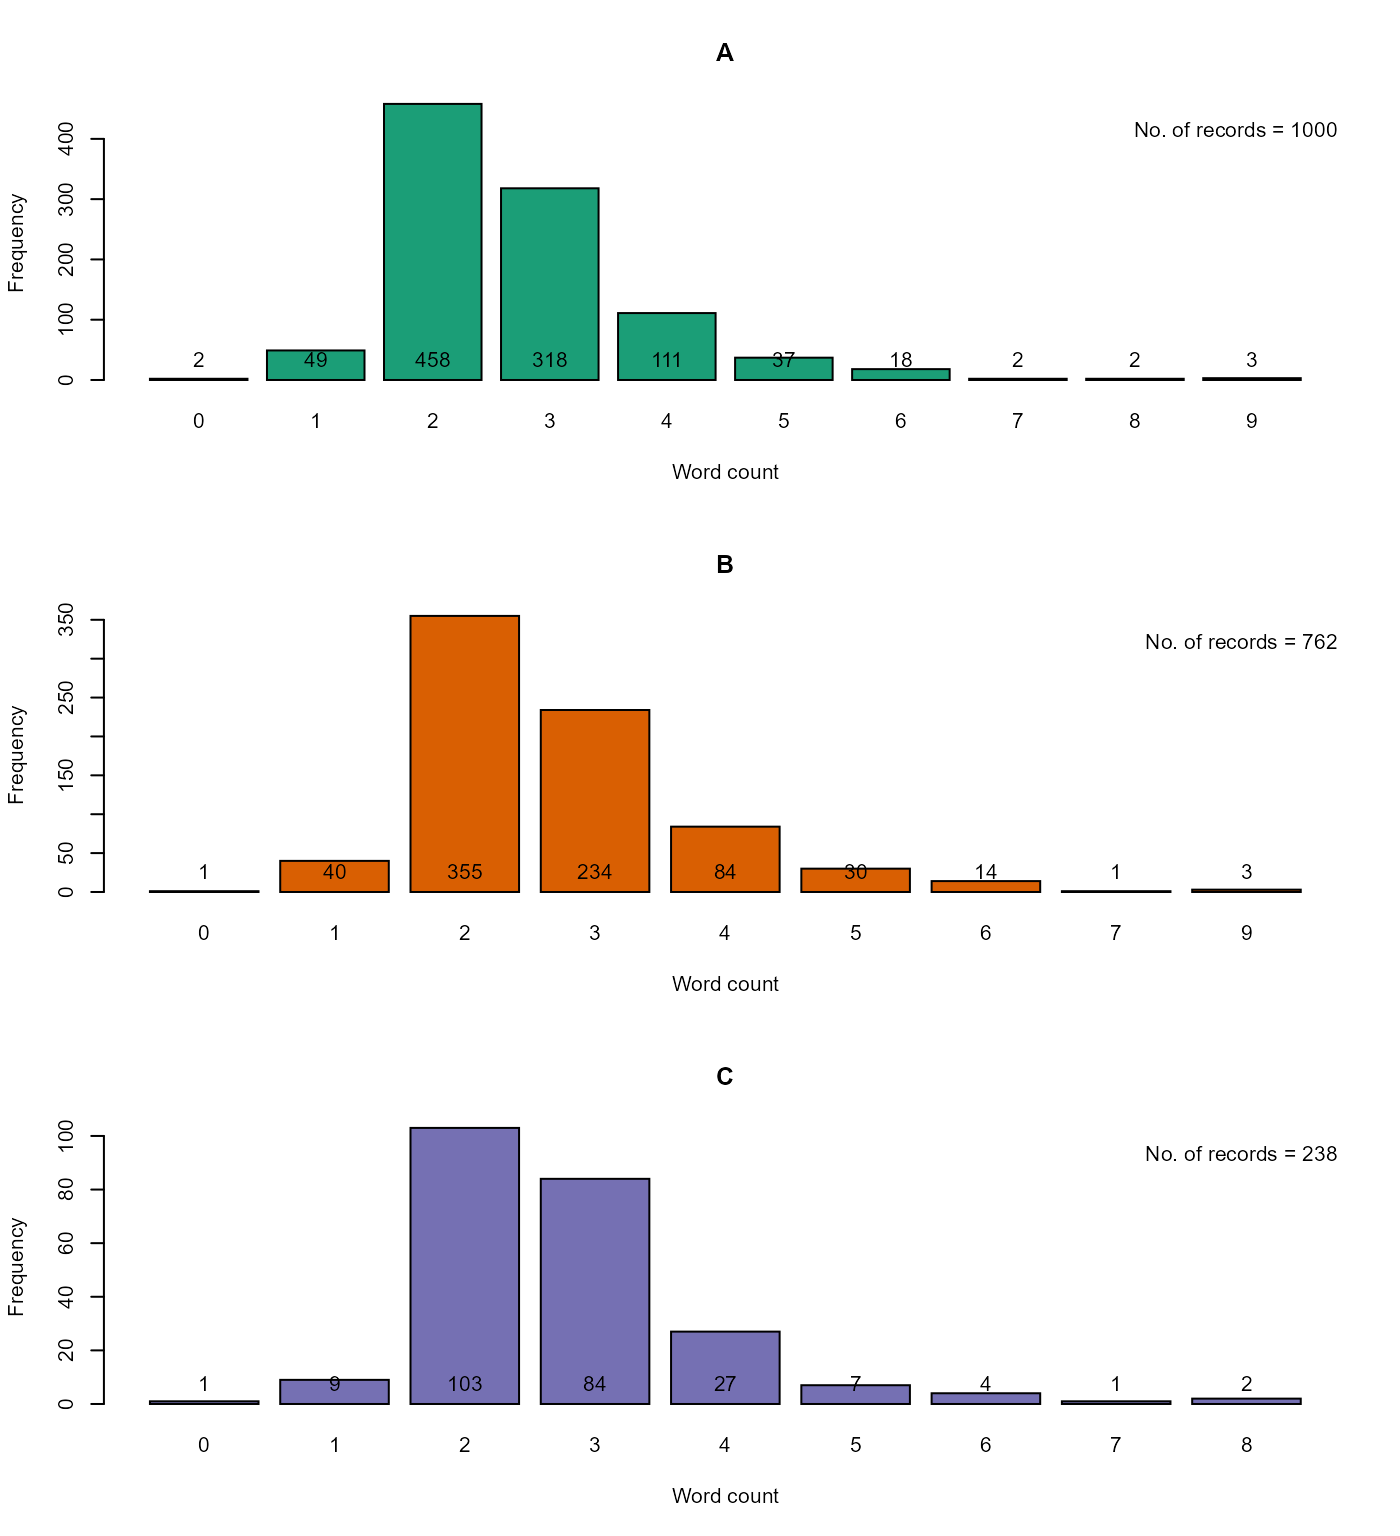
\includegraphics{Introduction_files/figure-latex/unnamed-chunk-61-1.pdf}

\textbf{Fig. 6.} The keyword counts in the database fields considered
for identification of probable duplicates for \textbf{A.}~the entire
\texttt{GN1000} dataset, \textbf{B.}~the probable duplicate records
alone and \textbf{C.}~the unique records alone.

\hypertarget{citing-pgrdup}{%
\subsection{\texorpdfstring{Citing
\texttt{PGRdup}}{Citing PGRdup}}\label{citing-pgrdup}}

\begin{Shaded}
\begin{Highlighting}[]
\KeywordTok{citation}\NormalTok{(}\StringTok{"PGRdup"}\NormalTok{)}
\end{Highlighting}
\end{Shaded}

\begin{verbatim}

To cite the R package 'PGRdup' in publications use:

  Aravind, J., Radhamani, J., Kalyani Srinivasan, Ananda Subhash, B., and Tyagi, R. K.  (2020).  PGRdup:
  Discover Probable Duplicates in Plant Genetic Resources Collections. R package version 0.2.3.6,
  https://github.com/aravind-j/PGRdup,https://cran.r-project.org/package=PGRdup.

A BibTeX entry for LaTeX users is

  @Manual{,
    title = {PGRdup: Discover Probable Duplicates in Plant Genetic Resources Collections},
    author = {J. Aravind and J. Radhamani and {Kalyani Srinivasan} and B. {Ananda Subhash} and Rishi Kumar Tyagi},
    year = {2020},
    note = {R package version 0.2.3.6},
    note = {https://github.com/aravind-j/PGRdup,},
    note = {https://cran.r-project.org/package=PGRdup},
  }

This free and open-source software implements academic research by the authors and co-workers. If you use
it, please support the project by citing the package.
\end{verbatim}

\hypertarget{session-info}{%
\subsection{Session Info}\label{session-info}}

\begin{Shaded}
\begin{Highlighting}[]
\KeywordTok{sessionInfo}\NormalTok{()}
\end{Highlighting}
\end{Shaded}

\begin{verbatim}
R Under development (unstable) (2020-07-22 r78897)
Platform: x86_64-w64-mingw32/x64 (64-bit)
Running under: Windows 10 x64 (build 19041)

Matrix products: default

locale:
[1] LC_COLLATE=English_India.1252  LC_CTYPE=English_India.1252    LC_MONETARY=English_India.1252
[4] LC_NUMERIC=C                   LC_TIME=English_India.1252    

attached base packages:
[1] stats     graphics  grDevices utils     datasets  methods   base     

other attached packages:
[1] PGRdup_0.2.3.6     gridExtra_2.3      wordcloud_2.6      RColorBrewer_1.1-2 diagram_1.6.4      shape_1.4.4       

loaded via a namespace (and not attached):
 [1] Rcpp_1.0.5             stringdist_0.9.6       prettyunits_1.1.1      ps_1.3.3               assertthat_0.2.1      
 [6] rprojroot_1.3-2        digest_0.6.25          R6_2.4.1               backports_1.1.8        evaluate_0.14         
[11] highr_0.8              httr_1.4.2             ggplot2_3.3.2          pillar_1.4.6           rlang_0.4.7           
[16] curl_4.3               rstudioapi_0.11.0-9000 data.table_1.13.0      callr_3.4.3            rmarkdown_2.3         
[21] labeling_0.3           desc_1.2.0             devtools_2.3.1         stringr_1.4.0          RCurl_1.98-1.2        
[26] igraph_1.2.5           munsell_0.5.0          compiler_4.1.0         xfun_0.16              microbenchmark_1.4-7  
[31] pkgconfig_2.0.3        pkgbuild_1.1.0         htmltools_0.5.0        tidyselect_1.1.0       tibble_3.0.3          
[36] roxygen2_7.1.1         XML_3.99-0.5           fansi_0.4.1            crayon_1.3.4           dplyr_1.0.0           
[41] withr_2.2.0            bitops_1.0-6           grid_4.1.0             gtable_0.3.0           lifecycle_0.2.0       
[46] magrittr_1.5           scales_1.1.1           cli_2.0.2              stringi_1.4.6          farver_2.0.3          
[51] fs_1.4.2               remotes_2.2.0          testthat_2.3.2         xml2_1.3.2             ellipsis_0.3.1        
[56] generics_0.0.2         vctrs_0.3.2            tools_4.1.0            glue_1.4.1             purrr_0.3.4           
[61] processx_3.4.3         pkgload_1.1.0          parallel_4.1.0         yaml_2.2.1             colorspace_1.4-1      
[66] sessioninfo_1.1.1      memoise_1.1.0          knitr_1.29             usethis_1.6.1         
\end{verbatim}

\hypertarget{references}{%
\subsection*{References}\label{references}}
\addcontentsline{toc}{subsection}{References}

\hypertarget{refs}{}
\leavevmode\hypertarget{ref-knupffer1988european}{}%
Knüpffer, H. 1988. ``The European Barley Database of the ECP/GR: An
Introduction.'' \emph{Die Kulturpflanze} 36 (1): 135--62.
\url{https://doi.org/https://doi.org/10.1007/BF01986957}.

\leavevmode\hypertarget{ref-kfj97}{}%
Knüpffer, H., L. Frese, and M. W. M. Jongen. 1997. ``Using Central Crop
Databases: Searching for Duplicates and Gaps.'' In \emph{Central Crop
Databases: Tools for Plant Genetic Resources Management. Report of a
Workshop, Budapest, Hungary, 13-16 October 1996}, edited by E. Lipman,
M. W. M. Jongen, T. J. L. van Hintum, T. Gass, and L. Maggioni, 67--77.
Rome, Italy and Wageningen, The Netherlands: International Plant Genetic
Resources Institute and Centre for Genetic Resources.
\url{https://www.bioversityinternational.org/index.php?id=244\&tx_news_pi1\%5Bnews\%5D=334\&cHash=3738ae238a450ff71bb1cb087687ac9c}.

\leavevmode\hypertarget{ref-p00}{}%
Philips, Lawrence. 2000. ``The Double Metaphone Search Algorithm.''
\emph{C/C++ Users Journal} 18 (6): 38--43.
\url{http://dl.acm.org/citation.cfm?id=349124.349132}.

\leavevmode\hypertarget{ref-van2014stringdist}{}%
van der Loo, M. P. J. 2014. ``The Stringdist Package for Approximate
String Matching.'' \emph{R Journal} 6 (1): 111--22.
\url{https://journal.r-project.org/archive/2014/RJ-2014-011/index.html}.

\end{document}
